% Capitolul 13: Foundation models și predicție conformală
% Analiza avansată a seriilor de timp și previziune -- Programul de master Statistică aplicată și data science, anul I, semestrul 2, Academia de Studii Economice din București
% GENERAT de latex/build_chapter13.py -- modificați generatorul, nu acest fișier.

\newcommand{\coursename}{Analiza avansată a seriilor de timp și previziune}
\def\atslang{ro}
% Preambul comun ATS -- Analiza avansată a seriilor de timp și previziune / Advanced Time Series Analysis and Forecasting
% (Beamer, 16:9). Același design ca MFM, SFM și TSA (copiat din TSA, 5 octombrie 2026). Înainte de % Preambul comun ATS -- Analiza avansată a seriilor de timp și previziune / Advanced Time Series Analysis and Forecasting
% (Beamer, 16:9). Același design ca MFM, SFM și TSA (copiat din TSA, 5 octombrie 2026). Înainte de % Preambul comun ATS -- Analiza avansată a seriilor de timp și previziune / Advanced Time Series Analysis and Forecasting
% (Beamer, 16:9). Același design ca MFM, SFM și TSA (copiat din TSA, 5 octombrie 2026). Înainte de \input{../../latex/preamble} se definește
%   \newcommand{\coursename}{Advanced Time Series Analysis and Forecasting}          (EN)
%   \newcommand{\coursename}{Analiza avansată a seriilor de timp și previziune}       (RO)  și  \def\atslang{ro}
% Fișierele .tex se află în EN/Courses, EN/Seminars, RO/Cursuri, RO/Seminarii (două niveluri sub rădăcină).
% Deck-urile sînt generate de latex/build_chapterN.py / build_seminarN.py (vezi latex/ats_build.py).

\documentclass[9pt, aspectratio=169, t]{beamer}
\providecommand{\coursename}{Advanced Time Series Analysis and Forecasting}

% Ensure content fits on slides
\setbeamersize{text margin left=8mm, text margin right=8mm}
% Smaller institute font (title page)
\setbeamerfont{institute}{size=\footnotesize}

%=============================================================================
% THEME AND STYLE CONFIGURATION
%=============================================================================
\usetheme{default}
% Using default theme for clean header/footer control

% Color Palette (matching Redispatch PDF)
\definecolor{MainBlue}{RGB}{26, 58, 110}
\definecolor{AccentBlue}{RGB}{26, 58, 110}
\definecolor{IDAred}{RGB}{205, 0, 0}
\definecolor{DarkGray}{RGB}{51, 51, 51}
\definecolor{MediumGray}{RGB}{128, 128, 128}
\definecolor{LightGray}{RGB}{248, 248, 248}
\definecolor{VeryLightGray}{RGB}{235, 235, 235}
\definecolor{KeynoteGray}{RGB}{218, 218, 218}
\definecolor{SectionGray}{RGB}{120, 120, 120}
\definecolor{FooterGray}{RGB}{100, 100, 100}
\definecolor{Crimson}{RGB}{220, 53, 69}
\definecolor{Forest}{RGB}{46, 125, 50}
\definecolor{Amber}{RGB}{181, 133, 63}
\definecolor{Orange}{RGB}{230, 126, 34}
\definecolor{Purple}{RGB}{142, 68, 173}

% Gradient background (exact Keynote 315° gradient: white to RGB 218,218,218)
\setbeamertemplate{background}{%
    \begin{tikzpicture}[remember picture, overlay]
        \shade[shading=axis, shading angle=315,
        top color=white, bottom color=KeynoteGray]
        (current page.south west) rectangle (current page.north east);
    \end{tikzpicture}%
}
% Fallback solid color for compatibility
\setbeamercolor{background canvas}{bg=}

\setbeamercolor{palette primary}{bg=MainBlue, fg=white}
\setbeamercolor{palette secondary}{bg=MainBlue!85, fg=white}
\setbeamercolor{palette tertiary}{bg=MainBlue!70, fg=white}
\setbeamercolor{structure}{fg=MainBlue}
\setbeamercolor{title}{fg=IDAred}
\setbeamercolor{frametitle}{fg=IDAred, bg=}
\setbeamercolor{block title}{bg=MainBlue, fg=white}
\setbeamercolor{block body}{bg=VeryLightGray, fg=DarkGray}
\setbeamercolor{block title alerted}{bg=Crimson, fg=white}
\setbeamercolor{block body alerted}{bg=Crimson!8, fg=DarkGray}
\setbeamercolor{block title example}{bg=Forest, fg=white}
\setbeamercolor{block body example}{bg=Forest!8, fg=DarkGray}
\setbeamercolor{item}{fg=MainBlue}

% Footer colors (override Madrid theme blue)
\setbeamercolor{author in head/foot}{fg=FooterGray, bg=}
\setbeamercolor{title in head/foot}{fg=FooterGray, bg=}
\setbeamercolor{date in head/foot}{fg=FooterGray, bg=}
\setbeamercolor{section in head/foot}{fg=FooterGray, bg=}
\setbeamercolor{subsection in head/foot}{fg=FooterGray, bg=}

% Bullet styles (apply everywhere including blocks)
\setbeamertemplate{itemize item}{\color{MainBlue}$\boxdot$}
\setbeamertemplate{itemize subitem}{\color{MainBlue}$\blacktriangleright$}
\setbeamertemplate{itemize subsubitem}{\color{MainBlue}\tiny$\bullet$}
\setbeamertemplate{itemize/enumerate body begin}{\normalsize}
\setbeamertemplate{itemize/enumerate subbody begin}{\normalsize}

% Item spacing - compact style
\setlength{\leftmargini}{10pt}       % Level 1: minimal indent
\setlength{\leftmarginii}{10pt}      % Level 2: minimal additional indent
% Compact list spacing (zero extra space before/after lists in blocks)
\makeatletter
\def\@listi{\leftmargin\leftmargini \topsep 0pt \parsep 0pt \itemsep 0pt}
\def\@listii{\leftmargin\leftmarginii \topsep 0pt \parsep 0pt \itemsep 0pt}
\makeatother

\setbeamertemplate{navigation symbols}{}

%=============================================================================
% CUSTOM HEADLINE
%=============================================================================
\setbeamertemplate{headline}{%
    \vskip10pt%
    \hbox to \paperwidth{%
        \hskip0.5cm%
        {\small\color{FooterGray}\renewcommand{\hyperlink}[2]{##2}\insertsectionhead}%
        \hfill%
        \textcolor{FooterGray}{\small\insertframenumber}%
        \hskip0.5cm%
    }%
    \vskip4pt%
    {\color{FooterGray}\hrule height 0.4pt}%
}

%=============================================================================
% CUSTOM FOOTER
%=============================================================================
\usepackage{fontawesome5}

\setbeamertemplate{footline}{%
    {\color{FooterGray}\hrule height 0.4pt}%
    \vskip4pt%
    \hbox to \paperwidth{%
        \hskip0.5cm%
        \textcolor{FooterGray}{\small\coursename}%
        \hfill%
        \raisebox{-0.1em}{%
            \begin{tikzpicture}[x=0.08em, y=0.08em, line width=0.4pt]
                \draw[FooterGray] (0,3) -- (1,4) -- (2,3.5) -- (3,5) -- (4,4) -- (5,6) -- (6,5.5) -- (7,4) -- (8,5) -- (9,7) -- (10,6) -- (11,5) -- (12,6.5) -- (13,8) -- (14,7) -- (15,6) -- (16,7.5) -- (17,9) -- (18,8) -- (19,7) -- (20,8.5) -- (21,10) -- (22,9) -- (23,8) -- (24,9.5);
            \end{tikzpicture}%
        }%
        \hskip0.5cm%
    }%
    \vskip6pt%
}

%=============================================================================
% PACKAGES
%=============================================================================
\usepackage[utf8]{inputenc}
\DeclareUnicodeCharacter{03B1}{\ensuremath{\alpha}}
\usepackage[T1]{fontenc}
\usepackage{amsmath, amssymb, amsthm}
\usepackage{mathtools}
\usepackage{bm}
\usepackage{tikz}
\usetikzlibrary{arrows.meta, positioning, shapes, calc, decorations.pathreplacing, shadings}
\usepackage{booktabs}
\usepackage{multirow}
\usepackage{array}
\usepackage{graphicx}
\usepackage{animate}
\usepackage{hyperref}
\usepackage{colortbl}
\usepackage{listings}
\lstset{language=Python, basicstyle=\ttfamily\scriptsize, keywordstyle=\color{MainBlue}\bfseries,
  commentstyle=\color{Forest}, stringstyle=\color{Crimson}, breaklines=true,
  frame=none, backgroundcolor=\color{VeryLightGray}, xleftmargin=2mm}
\hypersetup{colorlinks=true, linkcolor=MainBlue, urlcolor=MainBlue}
\graphicspath{{../../logos/}{../../charts/}{../../photos/}}
\usepackage{xcolor}
\hfuzz=2pt  % Suppress tiny overfull warnings (<2pt)
\vfuzz=2pt  % Suppress tiny vertical overfull warnings (<2pt)

%=============================================================================
% QUANTLET COMMANDS
%   \quantlet{<displayed name>}{<url>}       (generic)
%   \atsquantlet{Ch_05}{ATS_ch5_garch}       -> https://github.com/danpele/Advanced-Time-Series/tree/main/Quantlets/Ch_05/ATS_ch5_garch
%   \qlurl{<folder>} is defined per chapter by the generator (Quantlets/Ch_NN/<folder>)
%=============================================================================
\newcommand{\atsrepo}{https://github.com/danpele/Advanced-Time-Series}
\newcommand{\atsqlbase}{https://github.com/danpele/Advanced-Time-Series/tree/main/Quantlets}
\newcommand{\quantlet}[2]{%
    \hfill\href{#2}{%
        \raisebox{-0.15em}{
\includegraphics[height=0.7em]{ql_logo.png}}%
        \textcolor{MainBlue}{\tiny\ #1}%
    }%
}
\newcommand{\atsquantlet}[2]{\quantlet{\detokenize{#2}}{\atsqlbase/#1/#2}}

%=============================================================================
% NOTEBOOKS (Google Colab)
%   \colaburl{notebooks/EN/chapter5_seminar_notebook.ipynb} -> the Colab link of a file in the ATS repo
%   \nb: the chapter notebook (each seminar deck redefines it with \renewcommand)
%=============================================================================
\newcommand{\colaburl}[1]{https://colab.research.google.com/github/danpele/Advanced-Time-Series/blob/main/#1}
\newcommand{\nb}{https://colab.research.google.com/github/danpele/Advanced-Time-Series/tree/main/notebooks/EN}
\newcommand{\nbname}{notebooks/EN}

%=============================================================================
% SLIDE HELPERS (used by the generators; the same as in MFM)
%=============================================================================
% local font size for list bodies (the preamble forces \normalsize)
\newcommand{\itemsize}[1]{\setbeamertemplate{itemize/enumerate body begin}{#1}\setbeamertemplate{itemize/enumerate subbody begin}{#1}}
\newcommand{\intitle}[1]{{\hypersetup{urlcolor=white}#1}}   % white links inside coloured title bars
\newcommand{\imgcap}[1]{{\scriptsize #1}\\[0.5mm]}          % caption under a photo
\newcommand{\imgcredit}[2]{{\tiny\color{FooterGray}\href{#1}{#2}}}   % image credit: source URL, author/licence
\newcommand{\aiprompt}[1]{{\ttfamily\color{MainBlue}#1}}     % a prompt to an AI assistant

%=============================================================================
% SEMINARS: student version by default; the instructor wrapper *_solutions.tex sets \solutionstrue
%=============================================================================
\makeatletter\@ifundefined{ifsolutions}{\expandafter\newif\csname ifsolutions\endcsname}{}\makeatother
\newcommand{\solonly}[1]{\ifsolutions #1\fi}
\newcommand{\propsub}{\ifsolutions\else\framesubtitle{\ifdefined\atslang Rezolvarea se discută la seminar\else Solution discussed in class\fi}\fi}

%=============================================================================
% APPENDIX AND CHAPTER LINKS (latex/appendix_links.py writes the calls; it also re-declares these
% macros before \begin{document}, so the decks compile with or without this preamble block)
%=============================================================================
\providecommand{\atsapplink}[3]{\hypertarget{#2}{}\hyperlink{#1}{\beamergotobutton{#3}}}
\providecommand{\atsappback}[2]{\begin{tikzpicture}[remember picture,overlay]\node[anchor=south east] at ([xshift=-3mm,yshift=7mm]current page.south east){\hyperlink{#1}{\beamerreturnbutton{#2}}};\end{tikzpicture}}
\providecommand{\atschlink}[2]{\href{#1}{#2}}
\providecommand{\atschlinkt}[2]{\href{#1}{\usebeamercolor[fg]{frametitle}#2}}

%=============================================================================
% QUANTINAR COMMAND: link către un curs Quantinar (subiecte avansate)
%=============================================================================
\newcommand{\quantinar}[2]{%
    \href{#2}{%
        \raisebox{-0.15em}{
\includegraphics[height=0.8em]{qr_logo.png}}%
        \textcolor{MainBlue}{\scriptsize\ #1}%
    }%
}

%=============================================================================
% CUSTOM TITLE PAGE
%=============================================================================
\defbeamertemplate*{title page}{hybrid}[1][]
{
    \vspace{0.2cm}
    % Logos row - top header (with clickable links)
    \begin{center}
        \href{https://www.ase.ro}{
\includegraphics[height=1.0cm]{ase_logo.png}}\hspace{0.3cm}%
        \href{https://theida.net}{
\includegraphics[height=1.0cm]{ida_logo.png}}\hspace{0.3cm}%
        \href{https://blockchain-research-center.com}{
\includegraphics[height=1.0cm]{brc_logo.png}}\hspace{0.3cm}%
        \href{https://www.ai4efin.ase.ro}{
\includegraphics[height=1.0cm]{ai4efin_logo.png}}\hspace{0.3cm}%
        \href{https://ipe.ro/new}{
\includegraphics[height=1.0cm]{acad_logo.png}}\hspace{0.3cm}%
        \href{https://www.digital-finance-msca.com}{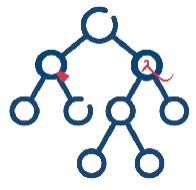
\includegraphics[height=1.0cm]{msca_logo.png}}%
    \end{center}

    \vspace{0.6cm}

    % Main title with Q logos on sides (with clickable links)
    \begin{center}
        \begin{minipage}{0.1\textwidth}
            \centering
            \href{https://quantlet.com}{
\includegraphics[height=1.1cm]{ql_logo.png}}
        \end{minipage}%
        \begin{minipage}{0.78\textwidth}
            \centering
            {\LARGE\bfseries\usebeamercolor[fg]{title}\inserttitle}

            \vspace{0.3cm}

            {\usebeamerfont{subtitle}\usebeamercolor[fg]{title}\insertsubtitle}
        \end{minipage}%
        \begin{minipage}{0.1\textwidth}
            \centering
            \href{https://quantinar.com}{
\includegraphics[height=1.1cm]{qr_logo.png}}
        \end{minipage}
    \end{center}

    \vspace{0.6cm}

    % Authors (left aligned)
    \hspace{0.5cm}{\usebeamerfont{author}\insertauthor}

    \vspace{0.3cm}

    % Institute/Affiliations (left aligned)
    \hspace{0.5cm}\begin{minipage}[t]{0.9\textwidth}
        \raggedright\small\insertinstitute
    \end{minipage}
}

%=============================================================================
% THEOREM ENVIRONMENTS
%=============================================================================
\theoremstyle{definition}
\setbeamertemplate{theorems}[numbered]
\ifdefined\atslang
\newtheorem{defn}{Definiție}
\newtheorem{thm}{Teoremă}
\newtheorem{prop}{Propoziție}
\newtheorem{rmk}{Observație}
\else
\newtheorem{defn}{Definition}
\newtheorem{thm}{Theorem}
\newtheorem{prop}{Proposition}
\newtheorem{rmk}{Remark}
\fi

%=============================================================================
% CENTRED MINIPAGE (no extra vertical space)
%=============================================================================
\newenvironment{cminipage}[1]{%
    \par\noindent\hfill\begin{minipage}{#1}\ignorespaces
}{%
    \end{minipage}\hfill\null\par
}

%=============================================================================
% CUSTOM COMMANDS
%=============================================================================
\newcommand{\E}{\mathbb{E}}
\newcommand{\Var}{\text{Var}}
\newcommand{\Cov}{\text{Cov}}
\newcommand{\Corr}{\text{Corr}}
\newcommand{\R}{\mathbb{R}}
\newcommand{\N}{\mathbb{N}}
\newcommand{\Z}{\mathbb{Z}}
\newcommand{\B}{\mathbf{B}}
\newcommand{\imark}{\textcolor{MainBlue}{\textbullet}}
\newcommand{\RMSE}{\text{RMSE}}
\newcommand{\MAE}{\text{MAE}}
\newcommand{\MAPE}{\text{MAPE}}

% Boldface vector/matrix commands (VAR, VECM, state space)
\newcommand{\bY}{\mathbf{Y}}
\newcommand{\bX}{\mathbf{X}}
\newcommand{\bA}{\mathbf{A}}
\newcommand{\bB}{\mathbf{B}}
\newcommand{\bepsilon}{\boldsymbol{\varepsilon}}
\newcommand{\bSigma}{\boldsymbol{\Sigma}}
\newcommand{\bPhi}{\boldsymbol{\Phi}}
\newcommand{\bGamma}{\boldsymbol{\Gamma}}
\newcommand{\bPi}{\boldsymbol{\Pi}}
\newcommand{\bc}{\mathbf{c}}
\newcommand{\balpha}{\boldsymbol{\alpha}}
\newcommand{\bbeta}{\boldsymbol{\beta}}
\newcommand{\bvarepsilon}{\boldsymbol{\varepsilon}}

% Seminar marks
\newcommand{\correct}{\textcolor{Forest}{\checkmark}}
\newcommand{\incorrect}{\textcolor{Crimson}{\texttimes}}
 se definește
%   \newcommand{\coursename}{Advanced Time Series Analysis and Forecasting}          (EN)
%   \newcommand{\coursename}{Analiza avansată a seriilor de timp și previziune}       (RO)  și  \def\atslang{ro}
% Fișierele .tex se află în EN/Courses, EN/Seminars, RO/Cursuri, RO/Seminarii (două niveluri sub rădăcină).
% Deck-urile sînt generate de latex/build_chapterN.py / build_seminarN.py (vezi latex/ats_build.py).

\documentclass[9pt, aspectratio=169, t]{beamer}
\providecommand{\coursename}{Advanced Time Series Analysis and Forecasting}

% Ensure content fits on slides
\setbeamersize{text margin left=8mm, text margin right=8mm}
% Smaller institute font (title page)
\setbeamerfont{institute}{size=\footnotesize}

%=============================================================================
% THEME AND STYLE CONFIGURATION
%=============================================================================
\usetheme{default}
% Using default theme for clean header/footer control

% Color Palette (matching Redispatch PDF)
\definecolor{MainBlue}{RGB}{26, 58, 110}
\definecolor{AccentBlue}{RGB}{26, 58, 110}
\definecolor{IDAred}{RGB}{205, 0, 0}
\definecolor{DarkGray}{RGB}{51, 51, 51}
\definecolor{MediumGray}{RGB}{128, 128, 128}
\definecolor{LightGray}{RGB}{248, 248, 248}
\definecolor{VeryLightGray}{RGB}{235, 235, 235}
\definecolor{KeynoteGray}{RGB}{218, 218, 218}
\definecolor{SectionGray}{RGB}{120, 120, 120}
\definecolor{FooterGray}{RGB}{100, 100, 100}
\definecolor{Crimson}{RGB}{220, 53, 69}
\definecolor{Forest}{RGB}{46, 125, 50}
\definecolor{Amber}{RGB}{181, 133, 63}
\definecolor{Orange}{RGB}{230, 126, 34}
\definecolor{Purple}{RGB}{142, 68, 173}

% Gradient background (exact Keynote 315° gradient: white to RGB 218,218,218)
\setbeamertemplate{background}{%
    \begin{tikzpicture}[remember picture, overlay]
        \shade[shading=axis, shading angle=315,
        top color=white, bottom color=KeynoteGray]
        (current page.south west) rectangle (current page.north east);
    \end{tikzpicture}%
}
% Fallback solid color for compatibility
\setbeamercolor{background canvas}{bg=}

\setbeamercolor{palette primary}{bg=MainBlue, fg=white}
\setbeamercolor{palette secondary}{bg=MainBlue!85, fg=white}
\setbeamercolor{palette tertiary}{bg=MainBlue!70, fg=white}
\setbeamercolor{structure}{fg=MainBlue}
\setbeamercolor{title}{fg=IDAred}
\setbeamercolor{frametitle}{fg=IDAred, bg=}
\setbeamercolor{block title}{bg=MainBlue, fg=white}
\setbeamercolor{block body}{bg=VeryLightGray, fg=DarkGray}
\setbeamercolor{block title alerted}{bg=Crimson, fg=white}
\setbeamercolor{block body alerted}{bg=Crimson!8, fg=DarkGray}
\setbeamercolor{block title example}{bg=Forest, fg=white}
\setbeamercolor{block body example}{bg=Forest!8, fg=DarkGray}
\setbeamercolor{item}{fg=MainBlue}

% Footer colors (override Madrid theme blue)
\setbeamercolor{author in head/foot}{fg=FooterGray, bg=}
\setbeamercolor{title in head/foot}{fg=FooterGray, bg=}
\setbeamercolor{date in head/foot}{fg=FooterGray, bg=}
\setbeamercolor{section in head/foot}{fg=FooterGray, bg=}
\setbeamercolor{subsection in head/foot}{fg=FooterGray, bg=}

% Bullet styles (apply everywhere including blocks)
\setbeamertemplate{itemize item}{\color{MainBlue}$\boxdot$}
\setbeamertemplate{itemize subitem}{\color{MainBlue}$\blacktriangleright$}
\setbeamertemplate{itemize subsubitem}{\color{MainBlue}\tiny$\bullet$}
\setbeamertemplate{itemize/enumerate body begin}{\normalsize}
\setbeamertemplate{itemize/enumerate subbody begin}{\normalsize}

% Item spacing - compact style
\setlength{\leftmargini}{10pt}       % Level 1: minimal indent
\setlength{\leftmarginii}{10pt}      % Level 2: minimal additional indent
% Compact list spacing (zero extra space before/after lists in blocks)
\makeatletter
\def\@listi{\leftmargin\leftmargini \topsep 0pt \parsep 0pt \itemsep 0pt}
\def\@listii{\leftmargin\leftmarginii \topsep 0pt \parsep 0pt \itemsep 0pt}
\makeatother

\setbeamertemplate{navigation symbols}{}

%=============================================================================
% CUSTOM HEADLINE
%=============================================================================
\setbeamertemplate{headline}{%
    \vskip10pt%
    \hbox to \paperwidth{%
        \hskip0.5cm%
        {\small\color{FooterGray}\renewcommand{\hyperlink}[2]{##2}\insertsectionhead}%
        \hfill%
        \textcolor{FooterGray}{\small\insertframenumber}%
        \hskip0.5cm%
    }%
    \vskip4pt%
    {\color{FooterGray}\hrule height 0.4pt}%
}

%=============================================================================
% CUSTOM FOOTER
%=============================================================================
\usepackage{fontawesome5}

\setbeamertemplate{footline}{%
    {\color{FooterGray}\hrule height 0.4pt}%
    \vskip4pt%
    \hbox to \paperwidth{%
        \hskip0.5cm%
        \textcolor{FooterGray}{\small\coursename}%
        \hfill%
        \raisebox{-0.1em}{%
            \begin{tikzpicture}[x=0.08em, y=0.08em, line width=0.4pt]
                \draw[FooterGray] (0,3) -- (1,4) -- (2,3.5) -- (3,5) -- (4,4) -- (5,6) -- (6,5.5) -- (7,4) -- (8,5) -- (9,7) -- (10,6) -- (11,5) -- (12,6.5) -- (13,8) -- (14,7) -- (15,6) -- (16,7.5) -- (17,9) -- (18,8) -- (19,7) -- (20,8.5) -- (21,10) -- (22,9) -- (23,8) -- (24,9.5);
            \end{tikzpicture}%
        }%
        \hskip0.5cm%
    }%
    \vskip6pt%
}

%=============================================================================
% PACKAGES
%=============================================================================
\usepackage[utf8]{inputenc}
\DeclareUnicodeCharacter{03B1}{\ensuremath{\alpha}}
\usepackage[T1]{fontenc}
\usepackage{amsmath, amssymb, amsthm}
\usepackage{mathtools}
\usepackage{bm}
\usepackage{tikz}
\usetikzlibrary{arrows.meta, positioning, shapes, calc, decorations.pathreplacing, shadings}
\usepackage{booktabs}
\usepackage{multirow}
\usepackage{array}
\usepackage{graphicx}
\usepackage{animate}
\usepackage{hyperref}
\usepackage{colortbl}
\usepackage{listings}
\lstset{language=Python, basicstyle=\ttfamily\scriptsize, keywordstyle=\color{MainBlue}\bfseries,
  commentstyle=\color{Forest}, stringstyle=\color{Crimson}, breaklines=true,
  frame=none, backgroundcolor=\color{VeryLightGray}, xleftmargin=2mm}
\hypersetup{colorlinks=true, linkcolor=MainBlue, urlcolor=MainBlue}
\graphicspath{{../../logos/}{../../charts/}{../../photos/}}
\usepackage{xcolor}
\hfuzz=2pt  % Suppress tiny overfull warnings (<2pt)
\vfuzz=2pt  % Suppress tiny vertical overfull warnings (<2pt)

%=============================================================================
% QUANTLET COMMANDS
%   \quantlet{<displayed name>}{<url>}       (generic)
%   \atsquantlet{Ch_05}{ATS_ch5_garch}       -> https://github.com/danpele/Advanced-Time-Series/tree/main/Quantlets/Ch_05/ATS_ch5_garch
%   \qlurl{<folder>} is defined per chapter by the generator (Quantlets/Ch_NN/<folder>)
%=============================================================================
\newcommand{\atsrepo}{https://github.com/danpele/Advanced-Time-Series}
\newcommand{\atsqlbase}{https://github.com/danpele/Advanced-Time-Series/tree/main/Quantlets}
\newcommand{\quantlet}[2]{%
    \hfill\href{#2}{%
        \raisebox{-0.15em}{
\includegraphics[height=0.7em]{ql_logo.png}}%
        \textcolor{MainBlue}{\tiny\ #1}%
    }%
}
\newcommand{\atsquantlet}[2]{\quantlet{\detokenize{#2}}{\atsqlbase/#1/#2}}

%=============================================================================
% NOTEBOOKS (Google Colab)
%   \colaburl{notebooks/EN/chapter5_seminar_notebook.ipynb} -> the Colab link of a file in the ATS repo
%   \nb: the chapter notebook (each seminar deck redefines it with \renewcommand)
%=============================================================================
\newcommand{\colaburl}[1]{https://colab.research.google.com/github/danpele/Advanced-Time-Series/blob/main/#1}
\newcommand{\nb}{https://colab.research.google.com/github/danpele/Advanced-Time-Series/tree/main/notebooks/EN}
\newcommand{\nbname}{notebooks/EN}

%=============================================================================
% SLIDE HELPERS (used by the generators; the same as in MFM)
%=============================================================================
% local font size for list bodies (the preamble forces \normalsize)
\newcommand{\itemsize}[1]{\setbeamertemplate{itemize/enumerate body begin}{#1}\setbeamertemplate{itemize/enumerate subbody begin}{#1}}
\newcommand{\intitle}[1]{{\hypersetup{urlcolor=white}#1}}   % white links inside coloured title bars
\newcommand{\imgcap}[1]{{\scriptsize #1}\\[0.5mm]}          % caption under a photo
\newcommand{\imgcredit}[2]{{\tiny\color{FooterGray}\href{#1}{#2}}}   % image credit: source URL, author/licence
\newcommand{\aiprompt}[1]{{\ttfamily\color{MainBlue}#1}}     % a prompt to an AI assistant

%=============================================================================
% SEMINARS: student version by default; the instructor wrapper *_solutions.tex sets \solutionstrue
%=============================================================================
\makeatletter\@ifundefined{ifsolutions}{\expandafter\newif\csname ifsolutions\endcsname}{}\makeatother
\newcommand{\solonly}[1]{\ifsolutions #1\fi}
\newcommand{\propsub}{\ifsolutions\else\framesubtitle{\ifdefined\atslang Rezolvarea se discută la seminar\else Solution discussed in class\fi}\fi}

%=============================================================================
% APPENDIX AND CHAPTER LINKS (latex/appendix_links.py writes the calls; it also re-declares these
% macros before \begin{document}, so the decks compile with or without this preamble block)
%=============================================================================
\providecommand{\atsapplink}[3]{\hypertarget{#2}{}\hyperlink{#1}{\beamergotobutton{#3}}}
\providecommand{\atsappback}[2]{\begin{tikzpicture}[remember picture,overlay]\node[anchor=south east] at ([xshift=-3mm,yshift=7mm]current page.south east){\hyperlink{#1}{\beamerreturnbutton{#2}}};\end{tikzpicture}}
\providecommand{\atschlink}[2]{\href{#1}{#2}}
\providecommand{\atschlinkt}[2]{\href{#1}{\usebeamercolor[fg]{frametitle}#2}}

%=============================================================================
% QUANTINAR COMMAND: link către un curs Quantinar (subiecte avansate)
%=============================================================================
\newcommand{\quantinar}[2]{%
    \href{#2}{%
        \raisebox{-0.15em}{
\includegraphics[height=0.8em]{qr_logo.png}}%
        \textcolor{MainBlue}{\scriptsize\ #1}%
    }%
}

%=============================================================================
% CUSTOM TITLE PAGE
%=============================================================================
\defbeamertemplate*{title page}{hybrid}[1][]
{
    \vspace{0.2cm}
    % Logos row - top header (with clickable links)
    \begin{center}
        \href{https://www.ase.ro}{
\includegraphics[height=1.0cm]{ase_logo.png}}\hspace{0.3cm}%
        \href{https://theida.net}{
\includegraphics[height=1.0cm]{ida_logo.png}}\hspace{0.3cm}%
        \href{https://blockchain-research-center.com}{
\includegraphics[height=1.0cm]{brc_logo.png}}\hspace{0.3cm}%
        \href{https://www.ai4efin.ase.ro}{
\includegraphics[height=1.0cm]{ai4efin_logo.png}}\hspace{0.3cm}%
        \href{https://ipe.ro/new}{
\includegraphics[height=1.0cm]{acad_logo.png}}\hspace{0.3cm}%
        \href{https://www.digital-finance-msca.com}{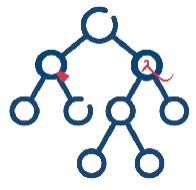
\includegraphics[height=1.0cm]{msca_logo.png}}%
    \end{center}

    \vspace{0.6cm}

    % Main title with Q logos on sides (with clickable links)
    \begin{center}
        \begin{minipage}{0.1\textwidth}
            \centering
            \href{https://quantlet.com}{
\includegraphics[height=1.1cm]{ql_logo.png}}
        \end{minipage}%
        \begin{minipage}{0.78\textwidth}
            \centering
            {\LARGE\bfseries\usebeamercolor[fg]{title}\inserttitle}

            \vspace{0.3cm}

            {\usebeamerfont{subtitle}\usebeamercolor[fg]{title}\insertsubtitle}
        \end{minipage}%
        \begin{minipage}{0.1\textwidth}
            \centering
            \href{https://quantinar.com}{
\includegraphics[height=1.1cm]{qr_logo.png}}
        \end{minipage}
    \end{center}

    \vspace{0.6cm}

    % Authors (left aligned)
    \hspace{0.5cm}{\usebeamerfont{author}\insertauthor}

    \vspace{0.3cm}

    % Institute/Affiliations (left aligned)
    \hspace{0.5cm}\begin{minipage}[t]{0.9\textwidth}
        \raggedright\small\insertinstitute
    \end{minipage}
}

%=============================================================================
% THEOREM ENVIRONMENTS
%=============================================================================
\theoremstyle{definition}
\setbeamertemplate{theorems}[numbered]
\ifdefined\atslang
\newtheorem{defn}{Definiție}
\newtheorem{thm}{Teoremă}
\newtheorem{prop}{Propoziție}
\newtheorem{rmk}{Observație}
\else
\newtheorem{defn}{Definition}
\newtheorem{thm}{Theorem}
\newtheorem{prop}{Proposition}
\newtheorem{rmk}{Remark}
\fi

%=============================================================================
% CENTRED MINIPAGE (no extra vertical space)
%=============================================================================
\newenvironment{cminipage}[1]{%
    \par\noindent\hfill\begin{minipage}{#1}\ignorespaces
}{%
    \end{minipage}\hfill\null\par
}

%=============================================================================
% CUSTOM COMMANDS
%=============================================================================
\newcommand{\E}{\mathbb{E}}
\newcommand{\Var}{\text{Var}}
\newcommand{\Cov}{\text{Cov}}
\newcommand{\Corr}{\text{Corr}}
\newcommand{\R}{\mathbb{R}}
\newcommand{\N}{\mathbb{N}}
\newcommand{\Z}{\mathbb{Z}}
\newcommand{\B}{\mathbf{B}}
\newcommand{\imark}{\textcolor{MainBlue}{\textbullet}}
\newcommand{\RMSE}{\text{RMSE}}
\newcommand{\MAE}{\text{MAE}}
\newcommand{\MAPE}{\text{MAPE}}

% Boldface vector/matrix commands (VAR, VECM, state space)
\newcommand{\bY}{\mathbf{Y}}
\newcommand{\bX}{\mathbf{X}}
\newcommand{\bA}{\mathbf{A}}
\newcommand{\bB}{\mathbf{B}}
\newcommand{\bepsilon}{\boldsymbol{\varepsilon}}
\newcommand{\bSigma}{\boldsymbol{\Sigma}}
\newcommand{\bPhi}{\boldsymbol{\Phi}}
\newcommand{\bGamma}{\boldsymbol{\Gamma}}
\newcommand{\bPi}{\boldsymbol{\Pi}}
\newcommand{\bc}{\mathbf{c}}
\newcommand{\balpha}{\boldsymbol{\alpha}}
\newcommand{\bbeta}{\boldsymbol{\beta}}
\newcommand{\bvarepsilon}{\boldsymbol{\varepsilon}}

% Seminar marks
\newcommand{\correct}{\textcolor{Forest}{\checkmark}}
\newcommand{\incorrect}{\textcolor{Crimson}{\texttimes}}
 se definește
%   \newcommand{\coursename}{Advanced Time Series Analysis and Forecasting}          (EN)
%   \newcommand{\coursename}{Analiza avansată a seriilor de timp și previziune}       (RO)  și  \def\atslang{ro}
% Fișierele .tex se află în EN/Courses, EN/Seminars, RO/Cursuri, RO/Seminarii (două niveluri sub rădăcină).
% Deck-urile sînt generate de latex/build_chapterN.py / build_seminarN.py (vezi latex/ats_build.py).

\documentclass[9pt, aspectratio=169, t]{beamer}
\providecommand{\coursename}{Advanced Time Series Analysis and Forecasting}

% Ensure content fits on slides
\setbeamersize{text margin left=8mm, text margin right=8mm}
% Smaller institute font (title page)
\setbeamerfont{institute}{size=\footnotesize}

%=============================================================================
% THEME AND STYLE CONFIGURATION
%=============================================================================
\usetheme{default}
% Using default theme for clean header/footer control

% Color Palette (matching Redispatch PDF)
\definecolor{MainBlue}{RGB}{26, 58, 110}
\definecolor{AccentBlue}{RGB}{26, 58, 110}
\definecolor{IDAred}{RGB}{205, 0, 0}
\definecolor{DarkGray}{RGB}{51, 51, 51}
\definecolor{MediumGray}{RGB}{128, 128, 128}
\definecolor{LightGray}{RGB}{248, 248, 248}
\definecolor{VeryLightGray}{RGB}{235, 235, 235}
\definecolor{KeynoteGray}{RGB}{218, 218, 218}
\definecolor{SectionGray}{RGB}{120, 120, 120}
\definecolor{FooterGray}{RGB}{100, 100, 100}
\definecolor{Crimson}{RGB}{220, 53, 69}
\definecolor{Forest}{RGB}{46, 125, 50}
\definecolor{Amber}{RGB}{181, 133, 63}
\definecolor{Orange}{RGB}{230, 126, 34}
\definecolor{Purple}{RGB}{142, 68, 173}

% Gradient background (exact Keynote 315° gradient: white to RGB 218,218,218)
\setbeamertemplate{background}{%
    \begin{tikzpicture}[remember picture, overlay]
        \shade[shading=axis, shading angle=315,
        top color=white, bottom color=KeynoteGray]
        (current page.south west) rectangle (current page.north east);
    \end{tikzpicture}%
}
% Fallback solid color for compatibility
\setbeamercolor{background canvas}{bg=}

\setbeamercolor{palette primary}{bg=MainBlue, fg=white}
\setbeamercolor{palette secondary}{bg=MainBlue!85, fg=white}
\setbeamercolor{palette tertiary}{bg=MainBlue!70, fg=white}
\setbeamercolor{structure}{fg=MainBlue}
\setbeamercolor{title}{fg=IDAred}
\setbeamercolor{frametitle}{fg=IDAred, bg=}
\setbeamercolor{block title}{bg=MainBlue, fg=white}
\setbeamercolor{block body}{bg=VeryLightGray, fg=DarkGray}
\setbeamercolor{block title alerted}{bg=Crimson, fg=white}
\setbeamercolor{block body alerted}{bg=Crimson!8, fg=DarkGray}
\setbeamercolor{block title example}{bg=Forest, fg=white}
\setbeamercolor{block body example}{bg=Forest!8, fg=DarkGray}
\setbeamercolor{item}{fg=MainBlue}

% Footer colors (override Madrid theme blue)
\setbeamercolor{author in head/foot}{fg=FooterGray, bg=}
\setbeamercolor{title in head/foot}{fg=FooterGray, bg=}
\setbeamercolor{date in head/foot}{fg=FooterGray, bg=}
\setbeamercolor{section in head/foot}{fg=FooterGray, bg=}
\setbeamercolor{subsection in head/foot}{fg=FooterGray, bg=}

% Bullet styles (apply everywhere including blocks)
\setbeamertemplate{itemize item}{\color{MainBlue}$\boxdot$}
\setbeamertemplate{itemize subitem}{\color{MainBlue}$\blacktriangleright$}
\setbeamertemplate{itemize subsubitem}{\color{MainBlue}\tiny$\bullet$}
\setbeamertemplate{itemize/enumerate body begin}{\normalsize}
\setbeamertemplate{itemize/enumerate subbody begin}{\normalsize}

% Item spacing - compact style
\setlength{\leftmargini}{10pt}       % Level 1: minimal indent
\setlength{\leftmarginii}{10pt}      % Level 2: minimal additional indent
% Compact list spacing (zero extra space before/after lists in blocks)
\makeatletter
\def\@listi{\leftmargin\leftmargini \topsep 0pt \parsep 0pt \itemsep 0pt}
\def\@listii{\leftmargin\leftmarginii \topsep 0pt \parsep 0pt \itemsep 0pt}
\makeatother

\setbeamertemplate{navigation symbols}{}

%=============================================================================
% CUSTOM HEADLINE
%=============================================================================
\setbeamertemplate{headline}{%
    \vskip10pt%
    \hbox to \paperwidth{%
        \hskip0.5cm%
        {\small\color{FooterGray}\renewcommand{\hyperlink}[2]{##2}\insertsectionhead}%
        \hfill%
        \textcolor{FooterGray}{\small\insertframenumber}%
        \hskip0.5cm%
    }%
    \vskip4pt%
    {\color{FooterGray}\hrule height 0.4pt}%
}

%=============================================================================
% CUSTOM FOOTER
%=============================================================================
\usepackage{fontawesome5}

\setbeamertemplate{footline}{%
    {\color{FooterGray}\hrule height 0.4pt}%
    \vskip4pt%
    \hbox to \paperwidth{%
        \hskip0.5cm%
        \textcolor{FooterGray}{\small\coursename}%
        \hfill%
        \raisebox{-0.1em}{%
            \begin{tikzpicture}[x=0.08em, y=0.08em, line width=0.4pt]
                \draw[FooterGray] (0,3) -- (1,4) -- (2,3.5) -- (3,5) -- (4,4) -- (5,6) -- (6,5.5) -- (7,4) -- (8,5) -- (9,7) -- (10,6) -- (11,5) -- (12,6.5) -- (13,8) -- (14,7) -- (15,6) -- (16,7.5) -- (17,9) -- (18,8) -- (19,7) -- (20,8.5) -- (21,10) -- (22,9) -- (23,8) -- (24,9.5);
            \end{tikzpicture}%
        }%
        \hskip0.5cm%
    }%
    \vskip6pt%
}

%=============================================================================
% PACKAGES
%=============================================================================
\usepackage[utf8]{inputenc}
\DeclareUnicodeCharacter{03B1}{\ensuremath{\alpha}}
\usepackage[T1]{fontenc}
\usepackage{amsmath, amssymb, amsthm}
\usepackage{mathtools}
\usepackage{bm}
\usepackage{tikz}
\usetikzlibrary{arrows.meta, positioning, shapes, calc, decorations.pathreplacing, shadings}
\usepackage{booktabs}
\usepackage{multirow}
\usepackage{array}
\usepackage{graphicx}
\usepackage{animate}
\usepackage{hyperref}
\usepackage{colortbl}
\usepackage{listings}
\lstset{language=Python, basicstyle=\ttfamily\scriptsize, keywordstyle=\color{MainBlue}\bfseries,
  commentstyle=\color{Forest}, stringstyle=\color{Crimson}, breaklines=true,
  frame=none, backgroundcolor=\color{VeryLightGray}, xleftmargin=2mm}
\hypersetup{colorlinks=true, linkcolor=MainBlue, urlcolor=MainBlue}
\graphicspath{{../../logos/}{../../charts/}{../../photos/}}
\usepackage{xcolor}
\hfuzz=2pt  % Suppress tiny overfull warnings (<2pt)
\vfuzz=2pt  % Suppress tiny vertical overfull warnings (<2pt)

%=============================================================================
% QUANTLET COMMANDS
%   \quantlet{<displayed name>}{<url>}       (generic)
%   \atsquantlet{Ch_05}{ATS_ch5_garch}       -> https://github.com/danpele/Advanced-Time-Series/tree/main/Quantlets/Ch_05/ATS_ch5_garch
%   \qlurl{<folder>} is defined per chapter by the generator (Quantlets/Ch_NN/<folder>)
%=============================================================================
\newcommand{\atsrepo}{https://github.com/danpele/Advanced-Time-Series}
\newcommand{\atsqlbase}{https://github.com/danpele/Advanced-Time-Series/tree/main/Quantlets}
\newcommand{\quantlet}[2]{%
    \hfill\href{#2}{%
        \raisebox{-0.15em}{
\includegraphics[height=0.7em]{ql_logo.png}}%
        \textcolor{MainBlue}{\tiny\ #1}%
    }%
}
\newcommand{\atsquantlet}[2]{\quantlet{\detokenize{#2}}{\atsqlbase/#1/#2}}

%=============================================================================
% NOTEBOOKS (Google Colab)
%   \colaburl{notebooks/EN/chapter5_seminar_notebook.ipynb} -> the Colab link of a file in the ATS repo
%   \nb: the chapter notebook (each seminar deck redefines it with \renewcommand)
%=============================================================================
\newcommand{\colaburl}[1]{https://colab.research.google.com/github/danpele/Advanced-Time-Series/blob/main/#1}
\newcommand{\nb}{https://colab.research.google.com/github/danpele/Advanced-Time-Series/tree/main/notebooks/EN}
\newcommand{\nbname}{notebooks/EN}

%=============================================================================
% SLIDE HELPERS (used by the generators; the same as in MFM)
%=============================================================================
% local font size for list bodies (the preamble forces \normalsize)
\newcommand{\itemsize}[1]{\setbeamertemplate{itemize/enumerate body begin}{#1}\setbeamertemplate{itemize/enumerate subbody begin}{#1}}
\newcommand{\intitle}[1]{{\hypersetup{urlcolor=white}#1}}   % white links inside coloured title bars
\newcommand{\imgcap}[1]{{\scriptsize #1}\\[0.5mm]}          % caption under a photo
\newcommand{\imgcredit}[2]{{\tiny\color{FooterGray}\href{#1}{#2}}}   % image credit: source URL, author/licence
\newcommand{\aiprompt}[1]{{\ttfamily\color{MainBlue}#1}}     % a prompt to an AI assistant

%=============================================================================
% SEMINARS: student version by default; the instructor wrapper *_solutions.tex sets \solutionstrue
%=============================================================================
\makeatletter\@ifundefined{ifsolutions}{\expandafter\newif\csname ifsolutions\endcsname}{}\makeatother
\newcommand{\solonly}[1]{\ifsolutions #1\fi}
\newcommand{\propsub}{\ifsolutions\else\framesubtitle{\ifdefined\atslang Rezolvarea se discută la seminar\else Solution discussed in class\fi}\fi}

%=============================================================================
% APPENDIX AND CHAPTER LINKS (latex/appendix_links.py writes the calls; it also re-declares these
% macros before \begin{document}, so the decks compile with or without this preamble block)
%=============================================================================
\providecommand{\atsapplink}[3]{\hypertarget{#2}{}\hyperlink{#1}{\beamergotobutton{#3}}}
\providecommand{\atsappback}[2]{\begin{tikzpicture}[remember picture,overlay]\node[anchor=south east] at ([xshift=-3mm,yshift=7mm]current page.south east){\hyperlink{#1}{\beamerreturnbutton{#2}}};\end{tikzpicture}}
\providecommand{\atschlink}[2]{\href{#1}{#2}}
\providecommand{\atschlinkt}[2]{\href{#1}{\usebeamercolor[fg]{frametitle}#2}}

%=============================================================================
% QUANTINAR COMMAND: link către un curs Quantinar (subiecte avansate)
%=============================================================================
\newcommand{\quantinar}[2]{%
    \href{#2}{%
        \raisebox{-0.15em}{
\includegraphics[height=0.8em]{qr_logo.png}}%
        \textcolor{MainBlue}{\scriptsize\ #1}%
    }%
}

%=============================================================================
% CUSTOM TITLE PAGE
%=============================================================================
\defbeamertemplate*{title page}{hybrid}[1][]
{
    \vspace{0.2cm}
    % Logos row - top header (with clickable links)
    \begin{center}
        \href{https://www.ase.ro}{
\includegraphics[height=1.0cm]{ase_logo.png}}\hspace{0.3cm}%
        \href{https://theida.net}{
\includegraphics[height=1.0cm]{ida_logo.png}}\hspace{0.3cm}%
        \href{https://blockchain-research-center.com}{
\includegraphics[height=1.0cm]{brc_logo.png}}\hspace{0.3cm}%
        \href{https://www.ai4efin.ase.ro}{
\includegraphics[height=1.0cm]{ai4efin_logo.png}}\hspace{0.3cm}%
        \href{https://ipe.ro/new}{
\includegraphics[height=1.0cm]{acad_logo.png}}\hspace{0.3cm}%
        \href{https://www.digital-finance-msca.com}{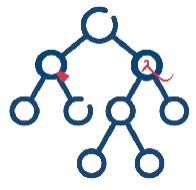
\includegraphics[height=1.0cm]{msca_logo.png}}%
    \end{center}

    \vspace{0.6cm}

    % Main title with Q logos on sides (with clickable links)
    \begin{center}
        \begin{minipage}{0.1\textwidth}
            \centering
            \href{https://quantlet.com}{
\includegraphics[height=1.1cm]{ql_logo.png}}
        \end{minipage}%
        \begin{minipage}{0.78\textwidth}
            \centering
            {\LARGE\bfseries\usebeamercolor[fg]{title}\inserttitle}

            \vspace{0.3cm}

            {\usebeamerfont{subtitle}\usebeamercolor[fg]{title}\insertsubtitle}
        \end{minipage}%
        \begin{minipage}{0.1\textwidth}
            \centering
            \href{https://quantinar.com}{
\includegraphics[height=1.1cm]{qr_logo.png}}
        \end{minipage}
    \end{center}

    \vspace{0.6cm}

    % Authors (left aligned)
    \hspace{0.5cm}{\usebeamerfont{author}\insertauthor}

    \vspace{0.3cm}

    % Institute/Affiliations (left aligned)
    \hspace{0.5cm}\begin{minipage}[t]{0.9\textwidth}
        \raggedright\small\insertinstitute
    \end{minipage}
}

%=============================================================================
% THEOREM ENVIRONMENTS
%=============================================================================
\theoremstyle{definition}
\setbeamertemplate{theorems}[numbered]
\ifdefined\atslang
\newtheorem{defn}{Definiție}
\newtheorem{thm}{Teoremă}
\newtheorem{prop}{Propoziție}
\newtheorem{rmk}{Observație}
\else
\newtheorem{defn}{Definition}
\newtheorem{thm}{Theorem}
\newtheorem{prop}{Proposition}
\newtheorem{rmk}{Remark}
\fi

%=============================================================================
% CENTRED MINIPAGE (no extra vertical space)
%=============================================================================
\newenvironment{cminipage}[1]{%
    \par\noindent\hfill\begin{minipage}{#1}\ignorespaces
}{%
    \end{minipage}\hfill\null\par
}

%=============================================================================
% CUSTOM COMMANDS
%=============================================================================
\newcommand{\E}{\mathbb{E}}
\newcommand{\Var}{\text{Var}}
\newcommand{\Cov}{\text{Cov}}
\newcommand{\Corr}{\text{Corr}}
\newcommand{\R}{\mathbb{R}}
\newcommand{\N}{\mathbb{N}}
\newcommand{\Z}{\mathbb{Z}}
\newcommand{\B}{\mathbf{B}}
\newcommand{\imark}{\textcolor{MainBlue}{\textbullet}}
\newcommand{\RMSE}{\text{RMSE}}
\newcommand{\MAE}{\text{MAE}}
\newcommand{\MAPE}{\text{MAPE}}

% Boldface vector/matrix commands (VAR, VECM, state space)
\newcommand{\bY}{\mathbf{Y}}
\newcommand{\bX}{\mathbf{X}}
\newcommand{\bA}{\mathbf{A}}
\newcommand{\bB}{\mathbf{B}}
\newcommand{\bepsilon}{\boldsymbol{\varepsilon}}
\newcommand{\bSigma}{\boldsymbol{\Sigma}}
\newcommand{\bPhi}{\boldsymbol{\Phi}}
\newcommand{\bGamma}{\boldsymbol{\Gamma}}
\newcommand{\bPi}{\boldsymbol{\Pi}}
\newcommand{\bc}{\mathbf{c}}
\newcommand{\balpha}{\boldsymbol{\alpha}}
\newcommand{\bbeta}{\boldsymbol{\beta}}
\newcommand{\bvarepsilon}{\boldsymbol{\varepsilon}}

% Seminar marks
\newcommand{\correct}{\textcolor{Forest}{\checkmark}}
\newcommand{\incorrect}{\textcolor{Crimson}{\texttimes}}


\newcommand{\qlurl}[1]{https://github.com/danpele/Advanced-Time-Series/tree/main/Quantlets/Ch_13/#1}

% Clickable citations (DOIs verified via Crossref)
\newcommand{\refAks}{\href{https://arxiv.org/abs/2410.10393}{Aksu et al.\ (2024)}}
\newcommand{\refAns}{\href{https://arxiv.org/abs/2403.07815}{Ansari et al.\ (2024)}}
\newcommand{\refAnsB}{\href{https://arxiv.org/abs/2510.15821}{Ansari et al.\ (2025)}}
\newcommand{\refAue}{\href{https://arxiv.org/abs/2505.23719}{Auer et al.\ (2025)}}
\newcommand{\refBom}{\href{https://arxiv.org/abs/2108.07258}{Bommasani et al.\ (2021)}}
\newcommand{\refBri}{\href{https://arxiv.org/abs/2607.05291}{Brini (2026)}}
\newcommand{\refCoh}{\href{https://arxiv.org/abs/2505.14766}{Cohen et al.\ (2025)}}
\newcommand{\refDas}{\href{https://arxiv.org/abs/2310.10688}{Das et al.\ (2024)}}
\newcommand{\refEdw}{\href{https://arxiv.org/abs/2405.13867}{Edwards et al.\ (2024)}}
\newcommand{\refGar}{\href{https://arxiv.org/abs/2310.03589}{Garza et al.\ (2023)}}
\newcommand{\refGarB}{\href{https://arxiv.org/abs/2603.08707}{Garza et al.\ (2026)}}
\newcommand{\refGoe}{\href{https://arxiv.org/abs/2505.11163}{Goel et al.\ (2025)}}
\newcommand{\refGos}{\href{https://arxiv.org/abs/2402.03885}{Goswami et al.\ (2024)}}
\newcommand{\refGru}{\href{https://arxiv.org/abs/2310.07820}{Gruver et al.\ (2023)}}
\newcommand{\refHof}{\href{https://arxiv.org/abs/2203.15556}{Hoffmann et al.\ (2022)}}
\newcommand{\refJin}{\href{https://arxiv.org/abs/2310.01728}{Jin et al.\ (2024)}}
\newcommand{\refKap}{\href{https://arxiv.org/abs/2001.08361}{Kaplan et al.\ (2020)}}
\newcommand{\refLiu}{\href{https://arxiv.org/abs/2511.11698}{Liu et al.\ (2025)}}
\newcommand{\refLTZ}{\href{https://arxiv.org/abs/2504.14765}{Lopez-Lira, Tang și Zhu (2025)}}
\newcommand{\refMey}{\href{https://arxiv.org/abs/2512.20761}{Meyer et al.\ (2025)}}
\newcommand{\refNie}{\href{https://arxiv.org/abs/2211.14730}{Nie et al.\ (2023)}}
\newcommand{\refPE}{\href{https://arxiv.org/abs/2607.02623}{Pan și Ezzat (2026)}}
\newcommand{\refRas}{\href{https://arxiv.org/abs/2310.08278}{Rasul et al.\ (2023)}}
\newcommand{\refRNW}{\href{https://arxiv.org/abs/2511.18578}{Rahimikia, Ni și Wang (2025)}}
\newcommand{\refShc}{\href{https://arxiv.org/abs/2509.26468}{Shchur et al.\ (2025)}}
\newcommand{\refShi}{\href{https://arxiv.org/abs/2405.15124}{Shi et al.\ (2024)}}
\newcommand{\refTan}{\href{https://arxiv.org/abs/2406.16964}{Tan et al.\ (2024)}}
\newcommand{\refVas}{\href{https://arxiv.org/abs/1706.03762}{Vaswani et al.\ (2017)}}
\newcommand{\refWoo}{\href{https://arxiv.org/abs/2402.02592}{Woo et al.\ (2024)}}
\newcommand{\refYao}{\href{https://arxiv.org/abs/2410.12360}{Yao et al.\ (2025)}}
\newcommand{\refZho}{\href{https://arxiv.org/abs/2302.11939}{Zhou et al.\ (2023)}}
\newcommand{\refBH}{\href{https://doi.org/10.1111/j.2517-6161.1995.tb02031.x}{Benjamini și Hochberg (1995)}}
\newcommand{\refBol}{\href{https://doi.org/10.1016/0304-4076(86)90063-1}{Bollerslev (1986)}}
\newcommand{\refChr}{\href{https://doi.org/10.2307/2527341}{Christoffersen (1998)}}
\newcommand{\refCor}{\href{https://doi.org/10.1093/jjfinec/nbp001}{Corsi (2009)}}
\newcommand{\refDem}{\href{https://jmlr.org/papers/v7/demsar06a.html}{Demšar (2006)}}
\newcommand{\refDM}{\href{https://doi.org/10.1080/07350015.1995.10524599}{Diebold și Mariano (1995)}}
\newcommand{\refEM}{\href{https://doi.org/10.1198/073500104000000370}{Engle și Manganelli (2004)}}
\newcommand{\refFW}{\href{https://doi.org/10.1145/5666.5673}{Fleming și Wallace (1986)}}
\newcommand{\refGR}{\href{https://doi.org/10.1198/016214506000001437}{Gneiting și Raftery (2007)}}
\newcommand{\refGW}{\href{https://doi.org/10.1111/j.1468-0262.2006.00718.x}{Giacomini și White (2006)}}
\newcommand{\refHAB}{\href{https://doi.org/10.1007/s10618-022-00894-5}{Hewamalage, Ackermann și Bergmeir (2023)}}
\newcommand{\refHLN}{\href{https://doi.org/10.1016/S0169-2070(96)00719-4}{Harvey, Leybourne și Newbold (1997)}}
\newcommand{\refHLNa}{\href{https://doi.org/10.3982/ECTA5771}{Hansen, Lunde și Nason (2011)}}
\newcommand{\refHF}{\href{https://doi.org/10.1016/j.ijforecast.2015.11.011}{Hong și Fan (2016)}}
\newcommand{\refHK}{\href{https://doi.org/10.1016/j.ijforecast.2006.03.001}{Hyndman și Koehler (2006)}}
\newcommand{\refHKSG}{\href{https://doi.org/10.1016/S0169-2070(01)00110-8}{Hyndman et al.\ (2002)}}
\newcommand{\refHol}{\href{https://www.jstor.org/stable/4615733}{Holm (1979)}}
\newcommand{\refKup}{\href{https://doi.org/10.3905/jod.1995.407942}{Kupiec (1995)}}
\newcommand{\refLim}{\href{https://doi.org/10.1016/j.ijforecast.2021.03.012}{Lim et al.\ (2021)}}
\newcommand{\refMak}{\href{https://doi.org/10.1016/j.ijforecast.2021.11.013}{Makridakis, Spiliotis și Assimakopoulos (2022)}}
\newcommand{\refOMI}{\href{https://web.archive.org/web/20220301022212/https://realized.oxford-man.ox.ac.uk/}{Heber et al.\ (2009)}}
\newcommand{\refOre}{\href{https://arxiv.org/abs/1905.10437}{Oreshkin et al.\ (2020)}}
\newcommand{\refPat}{\href{https://doi.org/10.1016/j.jeconom.2010.03.034}{Patton (2011)}}
\newcommand{\refPet}{\href{https://doi.org/10.1016/j.ijforecast.2021.11.001}{Petropoulos et al.\ (2022)}}
\newcommand{\refSal}{\href{https://doi.org/10.1016/j.ijforecast.2019.07.001}{Salinas et al.\ (2020)}}
\newcommand{\refZen}{\href{https://doi.org/10.1609/aaai.v37i9.26317}{Zeng et al.\ (2023)}}
\newcommand{\refZW}{\href{https://doi.org/10.1016/j.eneco.2017.12.016}{Ziel și Weron (2018)}}
\newcommand{\refAB}{\href{https://doi.org/10.1561/2200000101}{Angelopoulos și Bates (2023)}}
\newcommand{\refACT}{\href{https://arxiv.org/abs/2307.16895}{Angelopoulos, Candès și Tibshirani (2023)}}
\newcommand{\refBar}{\href{https://doi.org/10.1214/23-AOS2276}{Barber et al.\ (2023)}}
\newcommand{\refBarB}{\href{https://doi.org/10.1093/imaiai/iaaa017}{Foygel Barber et al.\ (2021)}}
\newcommand{\refCWZ}{\href{https://arxiv.org/abs/1802.06300}{Chernozhukov, Wüthrich și Zhu (2018)}}
\newcommand{\refGC}{\href{https://arxiv.org/abs/2106.00170}{Gibbs și Candès (2021)}}
\newcommand{\refGCb}{\href{https://jmlr.org/papers/v25/22-1218.html}{Gibbs și Candès (2024)}}
\newcommand{\refKB}{\href{https://doi.org/10.2307/1913643}{Koenker și Bassett (1978)}}
\newcommand{\refLei}{\href{https://doi.org/10.1080/01621459.2017.1307116}{Lei et al.\ (2018)}}
\newcommand{\refLW}{\href{https://doi.org/10.1111/rssb.12021}{Lei și Wasserman (2014)}}
\newcommand{\refOli}{\href{https://arxiv.org/abs/2203.15885}{Oliveira et al.\ (2024)}}
\newcommand{\refPap}{\href{https://doi.org/10.1007/3-540-36755-1_29}{Papadopoulos et al.\ (2002)}}
\newcommand{\refRPC}{\href{https://arxiv.org/abs/1905.03222}{Romano, Patterson și Candès (2019)}}
\newcommand{\refTBCR}{\href{https://arxiv.org/abs/1904.06019}{Tibshirani et al.\ (2019)}}
\newcommand{\refVGS}{\href{https://doi.org/10.1007/b106715}{Vovk, Gammerman și Shafer (2005)}}
\newcommand{\refVGSb}{\href{https://doi.org/10.1007/978-3-031-06649-8}{Vovk, Gammerman și Shafer (2022)}}
\newcommand{\refVov}{\href{https://proceedings.mlr.press/v25/vovk12.html}{Vovk (2012)}}
\newcommand{\refWin}{\href{https://doi.org/10.1080/01621459.1972.10481224}{Winkler (1972)}}
\newcommand{\refXX}{\href{https://proceedings.mlr.press/v139/xu21h.html}{Xu și Xie (2021)}}
\newcommand{\refXXb}{\href{https://doi.org/10.1109/TPAMI.2023.3272339}{Xu și Xie (2023)}}
\newcommand{\refZaf}{\href{https://arxiv.org/abs/2202.07282}{Zaffran et al.\ (2022)}}
\newcommand{\refCO}{\href{https://github.com/danpele/Conformal_Oracle}{Pele et al.\ (Conformal\_Oracle)}}
\newcommand{\refTV}{\href{https://github.com/danpele/TSFM_VaR_CEE}{Pele et al.\ (TSFM\_VaR\_CEE)}}

\title[Analiza avansată a seriilor de timp și previziune]{Analiza avansată a seriilor de timp și previziune}
\subtitle{Capitolul 13: Foundation models și predicție conformală}
\author[D.T. Pele]{Daniel Traian PELE}
\institute{Academia de Studii Economice din București\\
IDA Institute Digital Assets\\
Blockchain Research Center\\
AI4EFin Artificial Intelligence for Energy Finance\\
Academia Română, Institutul de Prognoză Economică\\
MSCA Digital Finance}
\date{}

%=============================================================================
\providecommand{\atsapplink}[3]{\hypertarget{#2}{}\hyperlink{#1}{\beamergotobutton{#3}}}  % APPLINKS-MACROS
\providecommand{\atsappback}[2]{\begin{tikzpicture}[remember picture,overlay]\node[anchor=south east] at ([xshift=-3mm,yshift=7mm]current page.south east){\hyperlink{#1}{\beamerreturnbutton{#2}}};\end{tikzpicture}}  % APPLINKS-MACROS
\providecommand{\atschlink}[2]{\href{#1}{#2}}  % APPLINKS-MACROS
\providecommand{\atschlinkt}[2]{\href{#1}{\usebeamercolor[fg]{frametitle}#2}}  % APPLINKS-MACROS
\begin{document}
%=============================================================================

{
\setbeamertemplate{headline}{}
\setbeamertemplate{footline}{}
\begin{frame}[noframenumbering]
    \titlepage
\end{frame}
}
% BEGIN-ACRONYMS (generat de latex/acronyms.py; nu editati manual)
\begin{frame}{Acronime folosite în acest material (1/2)}
\setbeamertemplate{itemize/enumerate body begin}{\tiny}
\begin{columns}[T]
\begin{column}{0.49\textwidth}
\begin{itemize}\setlength{\itemsep}{0pt}
    \item \textbf{ACI}: Adaptive Conformal Inference (inferență conformală adaptivă)
    \item \textbf{AI}: Artificial Intelligence (inteligență artificială)
    \item \textbf{AIC}: Akaike Information Criterion (criteriul informațional Akaike)
    \item \textbf{API}: Application Programming Interface (interfață de programare a aplicațiilor)
    \item \textbf{AR}: AutoRegressive (model); in event studies: Abnormal Return (model autoregresiv; în studiile de eveniment: randament anormal)
    \item \textbf{ARX}: AutoRegressive model with eXogenous variables (model autoregresiv cu variabile exogene)
    \item \textbf{BET}: Bucharest Exchange Trading (index) — indicele de referință al Bursei de Valori București
    \item \textbf{BH}: Benjamini–Hochberg (procedure) — procedura Benjamini–Hochberg
    \item \textbf{BOOM}: Benchmark Of Observability Metrics (benchmark de metrici de observabilitate (Toto))
    \item \textbf{CPM}: Contiguous Patch Masking (mascarea patch-urilor contigue)
    \item \textbf{CPU}: Central Processing Unit (procesorul central)
    \item \textbf{CQR}: Conformalized Quantile Regression (regresia cuantilică conformalizată)
    \item \textbf{CRPS}: Continuous Ranked Probability Score (scorul probabilistic continuu)
\end{itemize}
\end{column}
\begin{column}{0.49\textwidth}
\begin{itemize}\setlength{\itemsep}{0pt}
    \item \textbf{DM}: Diebold–Mariano (test) — testul Diebold–Mariano de comparare a prognozelor
    \item \textbf{DQ}: Dynamic Quantile (test of Engle and Manganelli) — testul dinamic pe cuantile al lui Engle și Manganelli
    \item \textbf{ENTSO-E}: European Network of Transmission System Operators for Electricity (Rețeaua europeană a operatorilor de transport și de sistem pentru energie electrică)
    \item \textbf{EODHD}: EOD Historical Data (market-data provider) — furnizor de date de piață
    \item \textbf{ETS}: Error, Trend, Seasonality (exponential smoothing state space models) — eroare, trend, sezonalitate (modele de netezire exponențială)
    \item \textbf{FDR}: False Discovery Rate (rata descoperirilor false)
    \item \textbf{FWER}: Family-Wise Error Rate (probabilitatea de cel puțin o eroare de tip I în familia de teste)
    \item \textbf{GARCH}: Generalised AutoRegressive Conditional Heteroskedasticity (heteroscedasticitate condiționată autoregresivă generalizată)
    \item \textbf{GIFT}: General Time Series Forecasting Model Evaluation (the GIFT-Eval benchmark) — benchmark general pentru evaluarea modelelor de prognoză
    \item \textbf{GPT-2}: Generative Pre-trained Transformer 2 (OpenAI language model) — model de limbaj al OpenAI, a doua generație
    \item \textbf{GPT4TS}: GPT for Time Series (One Fits All) — GPT pentru serii de timp (One Fits All)
    \item \textbf{GW}: Giacomini–White (test of conditional predictive ability) — testul Giacomini–White de capacitate predictivă condiționată
    \item \textbf{HAC}: Heteroskedasticity and Autocorrelation Consistent (standard errors) — erori standard robuste la heteroscedasticitate și autocorelație
\end{itemize}
\end{column}
\end{columns}
\end{frame}
\begin{frame}{Acronime folosite în acest material (2/2)}
\setbeamertemplate{itemize/enumerate body begin}{\tiny}
\begin{columns}[T]
\begin{column}{0.49\textwidth}
\begin{itemize}\setlength{\itemsep}{0pt}
    \item \textbf{HAR}: Heterogeneous AutoRegressive (model) — model autoregresiv heterogen
    \item \textbf{HICP}: Harmonised Index of Consumer Prices (indicele armonizat al prețurilor de consum (IAPC))
    \item \textbf{HLN}: Harvey–Leybourne–Newbold (small-sample correction of the DM test) — corecția Harvey–Leybourne–Newbold a testului DM pentru eșantioane mici
    \item \textbf{LLM}: Large Language Model (model lingvistic de mari dimensiuni)
    \item \textbf{LOTSA}: Large-scale Open Time Series Archive (arhiva deschisă de serii de timp de mari dimensiuni (Moirai))
    \item \textbf{MAE}: Mean Absolute Error (eroarea absolută medie)
    \item \textbf{MASE}: Mean Absolute Scaled Error (eroarea absolută medie scalată)
    \item \textbf{MCS}: Model Confidence Set (mulțimea de încredere a modelelor)
    \item \textbf{MOMENT}: MOMENT, a family of open time-series foundation models (familie de foundation models deschise pentru serii de timp)
    \item \textbf{MSE}: Mean Squared Error (eroarea pătratică medie)
    \item \textbf{NVIDIA}: NVIDIA Corporation (graphics processors) — compania NVIDIA (procesoare grafice)
    \item \textbf{OOD}: Out Of Distribution (în afara distribuției de antrenare)
    \item \textbf{PID}: Proportional--Integral--Derivative (controller) — controler proporțional--integral--derivat
\end{itemize}
\end{column}
\begin{column}{0.49\textwidth}
\begin{itemize}\setlength{\itemsep}{0pt}
    \item \textbf{QLIKE}: Quasi-LIKElihood loss (pierderea de tip cvasi-verosimilitate)
    \item \textbf{RLHF}: Reinforcement Learning from Human Feedback (învățare prin recompensă din evaluări umane)
    \item \textbf{RV}: Realised Variance (varianța realizată)
    \item \textbf{TS}: Time Series (in TS-Arena) — serii de timp (în numele TS-Arena)
    \item \textbf{TSA}: Time Series Analysis (Serii de timp, cursul de licență)
    \item \textbf{TVA}: Taxa pe valoarea adăugată
    \item \textbf{UE}: Uniunea Europeană
    \item \textbf{WQL}: Weighted Quantile Loss (pierderea cuantilică ponderată)
\end{itemize}
\end{column}
\end{columns}
\end{frame}
% END-ACRONYMS

\begin{frame}{Întrebarea de azi și traseul}
\itemsize{\small}
\begin{itemize}
    \item \textbf{Întrebarea}: poate un model preantrenat să prognozeze serii pe care nu le-a văzut niciodată și cum transformăm orice prognoză, preantrenată sau nu, în intervale a căror acoperire o putem garanta sau măcar controla?
    \begin{itemize}
        \item două jumătăți ale aceleiași probleme: acuratețea punctuală și a cuantilelor (foundation models), apoi o incertitudine onestă (predicția conformală)
    \end{itemize}
    \item \textbf{Traseul} capitolului
    \begin{itemize}
        \item preantrenarea: date, token-uri, patch-uri, legi de scalare; familiile de modele și alegerile de proiectare
        \item benchmark-uri, contaminare și testare pe multe serii; dovezi pe date românești și europene; LLM și critica lor
        \item predicția conformală: interschimbabilitate, split conformal, CQR, limitele acoperirii condiționate
        \item date dependente: ponderi, EnbPI, ACI, PID conformal; diagnosticare; calibrarea intervalelor produse de foundation models și VaR
    \end{itemize}
    \item Pornim de la \atschlink{https://danpele.github.io/Time-Series-Analysis/RO/Cursuri/capitol11_foundation_models_serii_timp.pdf}{TSA, Capitolul 11} (Chronos, TimesFM, Moirai, teste zero-shot, CRPS și WQL), de la \atschlink{https://danpele.github.io/Advanced-Time-Series/RO/Cursuri/capitol1_evaluarea_prognozelor.pdf}{Capitolul 1} (reguli de scor, DM, MCS), \atschlink{https://danpele.github.io/Advanced-Time-Series/RO/Cursuri/capitol9_var_es_backtesting.pdf}{Capitolul 9} (backtesting VaR, ACI pentru VaR) și \atschlink{https://danpele.github.io/Advanced-Time-Series/RO/Cursuri/capitol12_machine_learning_deep_learning.pdf}{Capitolul 12} (arhitecturi deep); Seminarul 13 are loc înaintea acestui curs
\end{itemize}
\end{frame}

\begin{frame}{Rezultatele învățării}
\itemsize{\small}
\begin{itemize}
    \item Explicați cum se preantrenează un foundation model pentru serii de timp: corpus, scalare, tokenizare sau patching, stratul de ieșire și funcția de pierdere
    \item Comparați familiile de modele și alegeți între folosirea zero-shot, fine-tuning și covariabilele în context
    \item Proiectați un benchmark fără scurgere de informație sau contaminare și testați diferențele pe multe serii cu corecții pentru testarea multiplă
    \item Demonstrați acoperirea metodelor split conformal și CQR și precizați ce nu poate garanta predicția conformală
    \item Aplicați predicția conformală ponderată, EnbPI, ACI și PID conformal pe date dependente, diagnosticați acoperirea și calibrați intervalele produse de foundation models
\end{itemize}
\end{frame}

\begin{frame}{Bibliografie, date și instrumente}
\itemsize{\small}
\begin{itemize}
    \item Foundation models: \refAns; \refAnsB; \refDas; \refWoo; \refAue; benchmark-uri: \refAks; \refShc
    \begin{itemize}
        \item Predicție conformală: \refVGSb; \refAB; \refRPC; \refBar; \refGC; \refACT; \refXX
        \item Critică și evaluare: \refTan; \refHAB; sinteză despre practica prognozei: \refPet
    \end{itemize}
    \item Quantlet-urile Python ale capitolului: \href{https://github.com/danpele/Advanced-Time-Series/tree/main/Quantlets/Ch_13}{Quantlets/Ch\_13}
    \begin{itemize}
        \item modele deschise pe un CPU: \texttt{chronos-forecasting} (Chronos-Bolt, Chronos-2), \texttt{timesfm} (TimesFM 2.5), \texttt{tirex-ts} (TiRex); metodele conformale, DM, MCS și backtesting-ul scrise în \texttt{numpy}
    \end{itemize}
    \item Notebook-ul cursului: \href{\colaburl{notebooks/EN/chapter13_lecture_notebook.ipynb}}{deschideți în Google Colab}
\end{itemize}
\end{frame}

\begin{frame}{Datele folosite în acest capitol}
\itemsize{\footnotesize}
\begin{center}
\scriptsize
\begin{tabular}{>{\raggedright\arraybackslash}p{3.9cm}>{\raggedright\arraybackslash}p{5.3cm}>{\raggedright\arraybackslash}p{2.9cm}}
\toprule
\textbf{Seria} & \textbf{Sursa} & \textbf{Eșantionul} \\
\midrule
Consumul de electricitate al României, orar & Energy-Charts (date de transparență ENTSO-E) & 2022 -- 30 septembrie 2026 \\
Temperatura aerului la București, orar & arhiva istorică Open-Meteo & 2022 -- 2026 \\
Inflația anuală HICP, 27 de țări UE & Eurostat, lunar & 2000 -- august 2026 \\
Varianța realizată, randamente de 5 minute & Bitcoin: Binance; S\&P 500: Oxford-Man \refOMI{} & 2018 -- 2026; 2000 -- 2022 \\
BET, S\&P 500, NVIDIA, zilnic & închideri zilnice EODHD & 2000 -- 2026 \\
\bottomrule
\end{tabular}
\end{center}
\begin{itemize}
    \item Randamentele sînt diferențe logaritmice înmulțite cu 100; varianța realizată este în procente la pătrat; orice prognoză folosește doar datele disponibile la momentul emiterii ei
\end{itemize}
\end{frame}

\begin{frame}{Două direcții de cercetare care s-au întîlnit}
\itemsize{\footnotesize}
\begin{columns}[T]
\begin{column}{0.4\textwidth}
\centering

\includegraphics[height=0.36\textheight]{ch13_royal_holloway.jpg}\\[1mm]
\imgcap{Royal Holloway, Universitatea din Londra: Founder's Building}
\imgcredit{https://commons.wikimedia.org/wiki/File:Founder's_Building,_Royal_Holloway,_University_of_London_-_Diliff.jpg}{Foto: Diliff (2015); CC BY-SA 3.0; Wikimedia Commons}
\end{column}
\begin{column}{0.58\textwidth}
\begin{itemize}
    \item Anii 1990--2005: predicția conformală la Royal Holloway: Vovk, Gammerman și Shafer, cu rădăcini în aleatorismul algoritmic al lui Kolmogorov \refVGS
    \item 2002--2018: split conformal (inductiv) \refPap; regresie fără ipoteze de distribuție \refLei; 2019: CQR \refRPC
    \item 2021--2023: serii de timp: ACI \refGC, EnbPI \refXX, PID conformal \refACT, dincolo de interschimbabilitate \refBar
    \item 2017--2025: Transformers \refVas, foundation models \refBom; pentru serii: Lag-Llama, TimesFM, Moirai, Chronos (2023--2024), TiRex, Chronos-2 (2025)
\end{itemize}
\end{column}
\end{columns}
\end{frame}

\begin{frame}{Cunoscut din TSA și elemente noi}
\itemsize{\small}
\begin{itemize}
    \item Cunoscut (\atschlink{https://danpele.github.io/Time-Series-Analysis/RO/Cursuri/capitol11_foundation_models_serii_timp.pdf}{TSA, Capitolul 11}): folosirea zero-shot a modelelor Chronos, TimesFM, Moirai și Lag-Llama; scalarea prin medie și cuantizarea, pe scurt; pierderea pinball, CRPS, WQL, MASE; primele avertismente despre contaminare
    \item Nou: instrumentele de cercetare
    \begin{itemize}
        \item alegerile de proiectare și consecințele lor (limitele de domeniu, straturi de cuantile, patching, covariabile în context), dovezile de scalare
        \item benchmark-uri cu ferestre preînregistrate după lansarea modelelor, teste pe multe serii cu corecțiile Holm și BH
        \item teoria conformală cu demonstrații, eșecul ei sub dependență și metodele online care o repară, cu diagnosticarea acoperirii
    \end{itemize}
    \item Studii de caz: Ansari et al.\ (2024), Tan et al.\ (2024), Romano--Patterson--Candès (2019), Gibbs--Candès (2021), Barber et al.\ (2023), Angelopoulos--Candès--Tibshirani (2023), Xu--Xie (2021), cu designul din lucrări, pe datele noastre
\end{itemize}
\end{frame}


%=============================================================================
\section{Preantrenarea pentru serii de timp}
%=============================================================================

\begin{frame}{Un foundation model ca prognozator amortizat}
\itemsize{\small}
\begin{itemize}
    \item \textbf{Preantrenarea}: $\hat\theta = \arg\min_\theta \sum_{s \in \mathcal D_{\mathrm{pre}}}\sum_t \ell\big(y^{(s)}_{t+1:t+H}, f_\theta(y^{(s)}_{t-C+1:t})\big)$ pe un corpus $\mathcal D_{\mathrm{pre}}$ format din multe serii
    \begin{itemize}
        \item $C$: lungimea contextului; $H$: orizontul; $\ell$: o regulă de scor (entropie încrucișată, pinball, log-verosimilitate negativă)
        \item termenul \textbf{foundation model} \refBom: antrenat o singură dată pe date diverse, apoi adaptat la multe sarcini
    \end{itemize}
    \item Folosirea \textbf{zero-shot}: $\hat\theta$ fixat, prognoza pentru o serie nouă este $f_{\hat\theta}(y_{T-C+1:T})$; niciun parametru nu se estimează pe seria-țintă
    \begin{itemize}
        \item rețeaua face pasul de estimare în interiorul trecerii înainte: inferența este amortizată pe corpus
    \end{itemize}
    \item Un model global din \atschlink{https://danpele.github.io/Advanced-Time-Series/RO/Cursuri/capitol12_machine_learning_deep_learning.pdf}{Capitolul 12} este antrenat pe seriile unui singur set de date; un foundation model, pe multe seturi de date, frecvențe și domenii
\end{itemize}
\end{frame}

\begin{frame}{Structuri comune între serii}
\itemsize{\small}
\begin{itemize}
    \item Formele se repetă între domenii: profiluri sezoniere, tendințe amortizate, salturi de nivel, grupări ale volatilității, intermitență
    \begin{itemize}
        \item după scalare, o curbă de consum și una de trafic web pot arăta la fel: modelul învață o distribuție a priori asupra formelor
    \end{itemize}
    \item Elemente care nu se transferă: economia unei serii anume (o modificare de taxe, o regulă de politică, un calendar al sărbătorilor)
    \begin{itemize}
        \item decît dacă este transmisă ca o covariabilă în context (Chronos-2) sau învățată prin fine-tuning
    \end{itemize}
    \item O rezervă de tip „no free lunch”: în medie pe toate procesele niciun prognozator nu cîștigă; preantrenarea ajută doar dacă seria-țintă seamănă cu corpusul
    \begin{itemize}
        \item randamentele financiare sînt aproape de o diferență de martingală: puțină formă de transferat, mult de supraajustat
    \end{itemize}
\end{itemize}
\end{frame}

\begin{frame}{Datele de preantrenare: volum și compoziție}
\itemsize{\small}
\begin{itemize}
    \item Chronos \refAns: seturi de date publice plus două augmentări: \textbf{TSMixup} (combinații convexe de serii reale) și \textbf{KernelSynth} (serii extrase din procese gaussiene cu nuclee compuse aleatoare)
    \item TimesFM \refDas: aproximativ $10^{11}$ momente de timp: Google Trends, accesări Wikipedia, serii sintetice și publice; Moirai \refWoo: LOTSA, peste 27 de miliarde de observații din nouă domenii
    \item Toto \refCoh: metrici de observabilitate ale unui furnizor cloud, un corpus de 4--10 ori mai mare decît al modelelor anterioare; GIFT-Eval \refAks: un set de preantrenare \textbf{fără scurgere} de circa 230 de miliarde de puncte
    \item Pentru noi compoziția contează mai mult decît volumul: seriile economice și financiare sînt o parte mică, de frecvență joasă, a oricărui corpus
\end{itemize}
\end{frame}

\begin{frame}{Tokenizarea: de la valori reale la un vocabular}
\itemsize{\small}
\begin{itemize}
    \item Chronos \refAns: \textbf{scalarea prin medie} $\tilde x_t = x_t/s$, $s = \frac1C\sum_{t \le C}|x_t|$ (doar contextul), apoi \textbf{intervale egale} pe $[-15, 15]$; 4096 de token-uri, inclusiv cele speciale
    \begin{itemize}
        \item modelul este un model de limbaj (T5) antrenat cu \textbf{entropia încrucișată}: prognoza este o distribuție categorială pe intervale, eșantionată autoregresiv
        \item nicio noțiune de distanță între token-uri: intervalele vecine sînt la fel de diferite ca cele îndepărtate, dacă datele nu arată altceva
    \end{itemize}
    \item Consecințe: rezoluția $30s/4092$; valorile peste $15s$ nu pot fi prognozate; invarianță la scală prin construcție
    \item LLMTime \refGru: cifrele ca token-uri de text; Lag-Llama \refRas: valori decalate ca variabile; modelele cu patch-uri: fără vocabular
\end{itemize}
\end{frame}

\begin{frame}{Tokenizatorul Chronos pe date reale}
\itemsize{\footnotesize}
\begin{center}
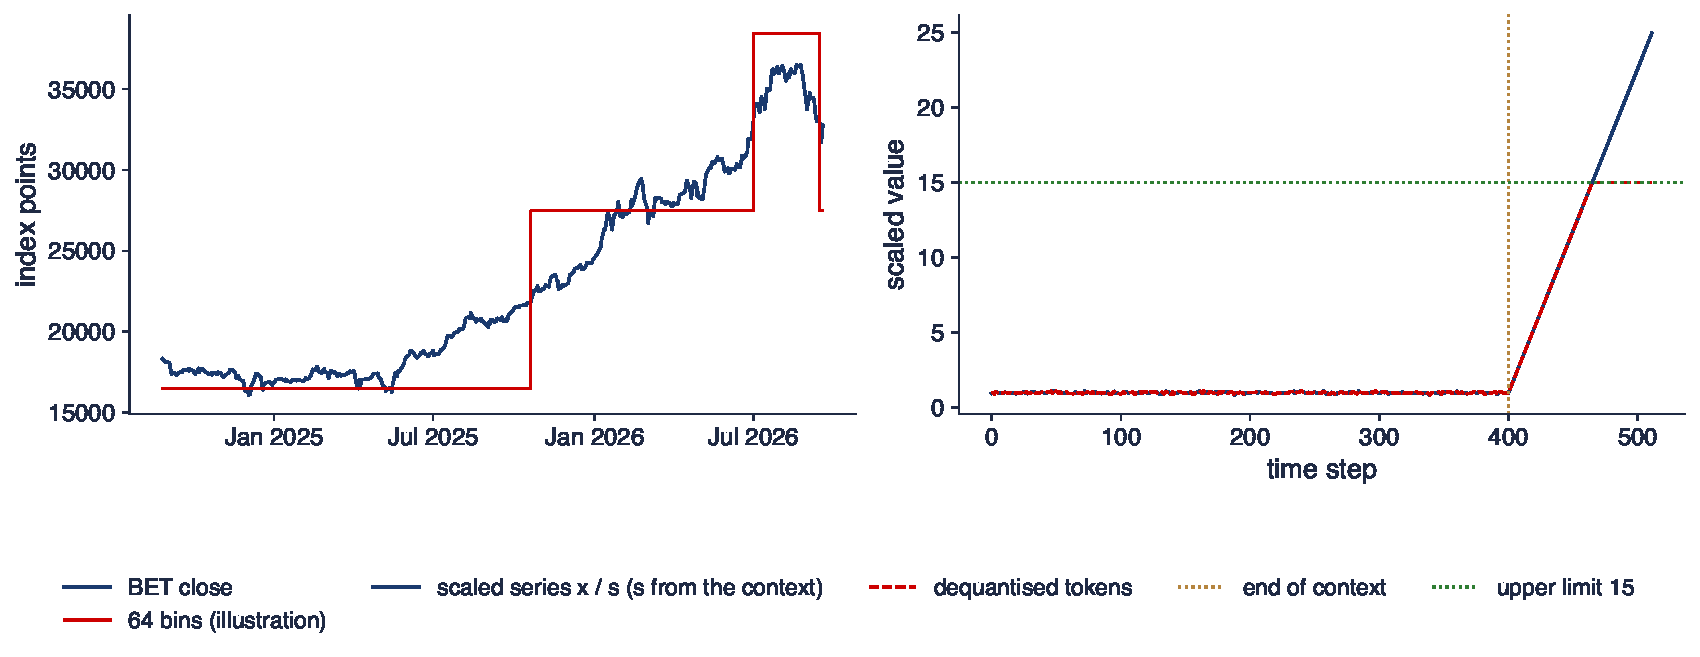
\includegraphics[width=0.97\textwidth,height=0.5\textheight,keepaspectratio]{ats_ch13_tokens.pdf}
\end{center}
\vspace{-0.25cm}
\begin{itemize}
    \item Stînga: închiderile BET, 27 august 2024 -- 18 septembrie 2026 ($C = 512$), și o cuantizare cu 64 de intervale (ilustrare); dreapta: un context în jurul valorii 1, urmat de o creștere pînă la un nivel de 25 de ori mai mare
\end{itemize}
\quantlet{ATS\_ch13\_pretraining}{\qlurl{ATS_ch13_pretraining}}
\end{frame}

\begin{frame}{Interpretarea tokenizatorului}
\itemsize{\small}
\begin{itemize}
    \item BET: $s = 23\,072$ puncte, lățimea intervalului 169{,}1 puncte, eroarea maximă de cuantizare 84{,}5 puncte: neglijabilă pentru prețuri, dar o pondere fixă din nivel
    \item Panoul din dreapta: scala este fixată de context, deci traiectoria care urcă peste $15s$ este tăiată: 42\% dintre pașii viitori sînt de neatins, ultimul cu o eroare de 40\%
    \item Seriile explozive (bule, \atschlink{https://danpele.github.io/Advanced-Time-Series/RO/Cursuri/capitol16_radacini_explozive_bule_speculative.pdf}{Capitolul 16}; hiperinflație) sînt în afara suportului unui vocabular scalat prin medie; Chronos-2 îl înlocuiește cu o transformare arcsinh și ieșiri sub formă de cuantile
\end{itemize}
\end{frame}

\begin{frame}{Patching și stratul de ieșire}
\itemsize{\small}
\begin{itemize}
    \item \textbf{Patching} \refNie: contextul se împarte în patch-uri de $P$ valori consecutive, iar fiecare patch devine un token; atenția costă $O((C/P)^2)$ în loc de $O(C^2)$
    \begin{itemize}
        \item TimesFM \refDas: patch-uri de intrare de 32, de ieșire de 128 (mai puțini pași autoregresivi); Chronos-Bolt și Chronos-2: patch-uri de 16; Moirai \refWoo: mai multe mărimi, după frecvență
    \end{itemize}
    \item Straturi de ieșire
    \begin{itemize}
        \item distribuție categorială pe intervale (Chronos); \textbf{strat de cuantile} antrenat cu pierderea pinball (Chronos-Bolt: 10\%--90\%; Chronos-2: 1\%--99\%; TimesFM 2.5, TiRex: decile)
        \item parametric: Student-$t$ (Lag-Llama \refRas), un amestec de distribuții (Moirai)
    \end{itemize}
    \item Cuantilele directe pe mai mulți pași (o singură trecere pentru $H$ pași) evită acumularea erorilor, dar dau distribuții predictive marginale, nu comune: funcționalele de traiectorie (un maxim, o sumă) cer atenție
\end{itemize}
\end{frame}

\begin{frame}{Legi de scalare}
\itemsize{\small}
\begin{itemize}
    \item Modelele de limbaj \refKap, \refHof: pierderea pe datele de test scade ca o lege de putere, $L(N) \approx (N_c/N)^{\alpha_N}$, în numărul de parametri $N$, în date și în calcul, pe mai multe ordine de mărime
    \item Serii de timp: Transformers de tip decoder-only arată aceleași legi de putere în parametri, date și calcul \refEdw; lungimea contextului interacționează cu volumul datelor \refShi
    \begin{itemize}
        \item în afara distribuției: log-verosimilitatea se scalează asemănător în și în afara distribuției, dar arhitectura contează; ajustările care ajută în distribuție pot reduce scalabilitatea OOD \refYao
    \end{itemize}
    \item O lege de scalare este o afirmație despre pierderea medie pe distribuția corpusului, nu despre o serie românească anume; modele mici (TiRex, 35 de milioane de parametri) le întrec pe cele mari în clasamentele publice \refAue
\end{itemize}
\end{frame}

\begin{frame}{Mărimea și acuratețea pe cele trei sarcini ale noastre}
\itemsize{\footnotesize}
\begin{center}
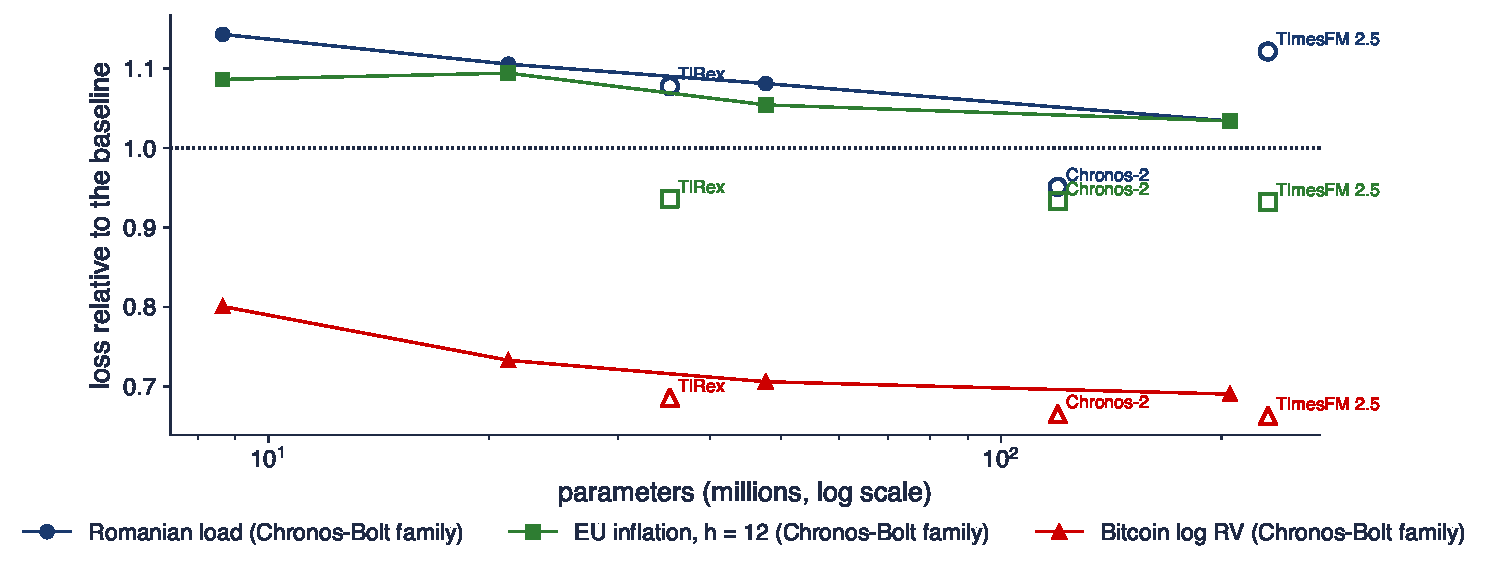
\includegraphics[width=0.97\textwidth,height=0.5\textheight,keepaspectratio]{ats_ch13_scaling.pdf}
\end{center}
\vspace{-0.25cm}
\begin{itemize}
    \item Pierderi relative la modelul de referință al fiecărei sarcini: consumul României (MAE / ARX expert, 2025--2026), inflația UE (MAE / mers aleator, $h = 12$, medie geometrică pe 27 de țări), log RV Bitcoin (MSE / HAR); parametrii numărați în modelele încărcate
\end{itemize}
\quantlet{ATS\_ch13\_pretraining}{\qlurl{ATS_ch13_pretraining}}
\end{frame}

\begin{frame}{Interpretarea relației dintre mărime și acuratețe}
\itemsize{\small}
\begin{itemize}
    \item Familia Chronos-Bolt (9--205 M parametri): consum 1{,}143 $\to$ 1{,}034, inflație 1{,}086 $\to$ 1{,}034, Bitcoin 0{,}800 $\to$ 0{,}690
    \item Între familii, mărimea nu dă clasamentul: Chronos-2 (119 M) 0{,}951 la consum; TiRex (35 M) 1{,}078; TimesFM 2.5 (231 M) 1{,}121
    \item În familia Chronos-Bolt pierderea scade odată cu mărimea pe toate cele trei sarcini (o excepție: mini la inflație); între familii, arhitectura, corpusul și rețeta de antrenare se schimbă împreună, deci trei sarcini nu fac un studiu de scalare
\end{itemize}
\end{frame}

\begin{frame}{Recapitulare: preantrenarea}
\itemsize{\small}
\begin{itemize}
    \item Preantrenarea amortizează estimarea pe un corpus; folosirea zero-shot rulează estimatorul într-o singură trecere înainte
    \item Scalarea prin medie și intervalele dau invarianță la scală, dar un domeniu limitat; patching și straturile de cuantile le înlocuiesc cu cuantile directe pe mai mulți pași
    \item Legile de scalare sînt valabile în medie pe corpusuri; pe o serie economică dată, proiectarea și datele contează mai mult decît mărimea
\end{itemize}
\end{frame}


%=============================================================================
\section{Familii de modele și alegeri de proiectare}
%=============================================================================

\begin{frame}{Principalele modele deschise}
\itemsize{\footnotesize}
\begin{center}
\scriptsize
\begin{tabular}{>{\raggedright\arraybackslash}p{2.2cm}>{\raggedright\arraybackslash}p{3.4cm}>{\raggedright\arraybackslash}p{2.0cm}>{\raggedright\arraybackslash}p{3.9cm}}
\toprule
\textbf{Modelul} & \textbf{Arhitectura} & \textbf{Parametri} & \textbf{Ieșirea} \\
\midrule
Chronos \refAns{} & T5 encoder--decoder pe token-uri & 20--710 M & categorială, traiectorii eșantionate \\
Chronos-Bolt & T5 pe patch-uri de 16 & 9--205 M & 9 cuantile, 10\%--90\%, 64 de pași \\
Chronos-2 \refAnsB{} & encoder cu atenție de grup & 119 M & 21 de cuantile, 1\%--99\%; covariabile \\
TimesFM 2.5 \refDas{} & decoder-only, patch-uri & 231 M & media și decilele \\
Moirai \refWoo{} & encoder mascat, atenție pe orice număr de variabile & 14--311 M & amestec de distribuții \\
Lag-Llama \refRas{} & decoder-only pe valori decalate & mic & Student-$t$ \\
MOMENT \refGos{} & encoder T5 mascat, multi-sarcină & 40--385 M & reconstrucție; straturi pe sarcină \\
TiRex \refAue{} & xLSTM & 35 M & decile \\
\bottomrule
\end{tabular}
\end{center}
\begin{itemize}
    \item Toto \refCoh{} (151 M, date de observabilitate) și Moirai 2.0 \refLiu{} sînt și ele deschise; TimeGPT \refGar{} este accesibil doar printr-un API cu plată
\end{itemize}
\end{frame}

\begin{frame}{Familia Chronos}
\itemsize{\small}
\begin{itemize}
    \item \textbf{Chronos} \refAns: rețeta modelelor de limbaj fără modificări; prognoze prin eșantionarea traiectoriilor de token-uri; rezultate zero-shot comparabile cu modele antrenate pe datele-țintă (Benchmark II din lucrare)
    \item \textbf{Chronos-Bolt}: intrări sub formă de patch-uri, decodor direct de cuantile; mult mai rapid; context de pînă la 2048, 64 de pași; cuantile doar între 10\% și 90\%
    \begin{itemize}
        \item un interval de 95\% sau un VaR 1\% nu se pot citi din ieșirea lui: cererea este tăiată la cel mai apropiat nivel antrenat
    \end{itemize}
    \item \textbf{Chronos-2} \refAnsB: atenția de grup împarte informația între seriile unui grup (variabile, serii înrudite, covariabile); \textbf{învățare în context} a efectelor covariabilelor
    \begin{itemize}
        \item antrenat în mare parte pe structuri multivariate sintetice impuse unor serii univariate; context de 8192; 21 de cuantile de la 1\% la 99\%; scalare arcsinh
    \end{itemize}
\end{itemize}
\end{frame}

\begin{frame}{TimesFM, Moirai, Lag-Llama, MOMENT}
\itemsize{\small}
\begin{itemize}
    \item \textbf{TimesFM} \refDas: decoder-only, patch-uri; patch-ul de ieșire mai lung decît cel de intrare; antrenat pe multe frecvențe; versiunea 2.5 adaugă un strat de cuantile și contexte lungi
    \item \textbf{Moirai} \refWoo: encoder mascat; mărimi de patch specifice frecvenței; atenția pe orice număr de variabile aplatizează intrările multivariate; ieșire sub formă de amestec (Student-$t$, log-normală, binomială negativă)
    \begin{itemize}
        \item Moirai 2.0 \refLiu: o simplificare decoder-only, mai mică și mai bună pe GIFT-Eval
    \end{itemize}
    \item \textbf{Lag-Llama} \refRas: un decodor de tip LLaMA ale cărui token-uri sînt vectori de valori decalate la multe decalaje sezoniere; strat Student-$t$; puternic după fine-tuning
    \item \textbf{MOMENT} \refGos: reconstrucție mascată pe Time series Pile; un singur encoder pentru prognoză, clasificare, detectarea anomaliilor și imputare
\end{itemize}
\end{frame}

\begin{frame}{Din nou recurente, observabilitate și un API închis}
\itemsize{\small}
\begin{itemize}
    \item \textbf{TiRex} \refAue: un xLSTM (celulele recurente din \atschlink{https://danpele.github.io/Advanced-Time-Series/RO/Cursuri/capitol12_machine_learning_deep_learning.pdf}{Capitolul 12}, cu porți exponențiale și memorie matriceală) păstrează o stare de-a lungul contextului: urmărirea stării pe orizonturi lungi
    \begin{itemize}
        \item mascarea patch-urilor contigue (CPM) la antrenare: modelul învață să prognozeze cu patch-uri lipsă, adică mai mulți pași fără reacție
    \end{itemize}
    \item \textbf{Toto} \refCoh: decoder-only pentru metrici multivariate de observabilitate; benchmark-ul BOOM (2807 serii); arată că alcătuirea pe domenii a corpusului determină rezultatele
    \item \textbf{TimeGPT} \refGar: ponderi închise și corpus nedezvăluit, în spatele unui API cu plată
    \begin{itemize}
        \item contaminarea nu poate fi verificată; rezultatele nu sînt reproductibile dacă serviciul schimbă modelul; datele ies din instituția dumneavoastră
    \end{itemize}
\end{itemize}
\end{frame}

\begin{frame}{Zero-shot, fine-tuning, covariabile în context}
\itemsize{\small}
\begin{itemize}
    \item \textbf{Zero-shot}: $f_{\hat\theta}(y_{T-C+1:T})$; fără antrenare, fără riscul ajustării; singurele alegeri sînt $C$ și modelul
    \item \textbf{Fine-tuning}: $\theta$ pornește de la $\hat\theta$, cîțiva pași de gradient pe datele-țintă (toate ponderile sau adaptoare precum LoRA)
    \begin{itemize}
        \item cere o împărțire de validare care respectă timpul (\atschlink{https://danpele.github.io/Advanced-Time-Series/RO/Cursuri/capitol12_machine_learning_deep_learning.pdf}{Capitolul 12}); poate uita distribuția a priori; pe serii economice scurte rareori merită
    \end{itemize}
    \item \textbf{Covariabile în context} (Chronos-2): se transmit valorile trecute ale lui $x_t$ și valorile viitoare ale regresorilor cunoscuți; modelul deduce efectul lor în timpul trecerii înainte
    \begin{itemize}
        \item învățarea încrucișată: prognoza în comun a unui lot de serii înrudite (toate cele 27 de țări UE la aceeași origine)
    \end{itemize}
    \item Covariabilele viitoare cunoscute trebuie să fie chiar cunoscute la origine: prognoze meteo, nu vremea realizată, cu excepția cazului în care se urmărește o limită superioară
\end{itemize}
\end{frame}

\begin{frame}{Patru prognoze zero-shot cu același model}
\itemsize{\footnotesize}
\begin{center}
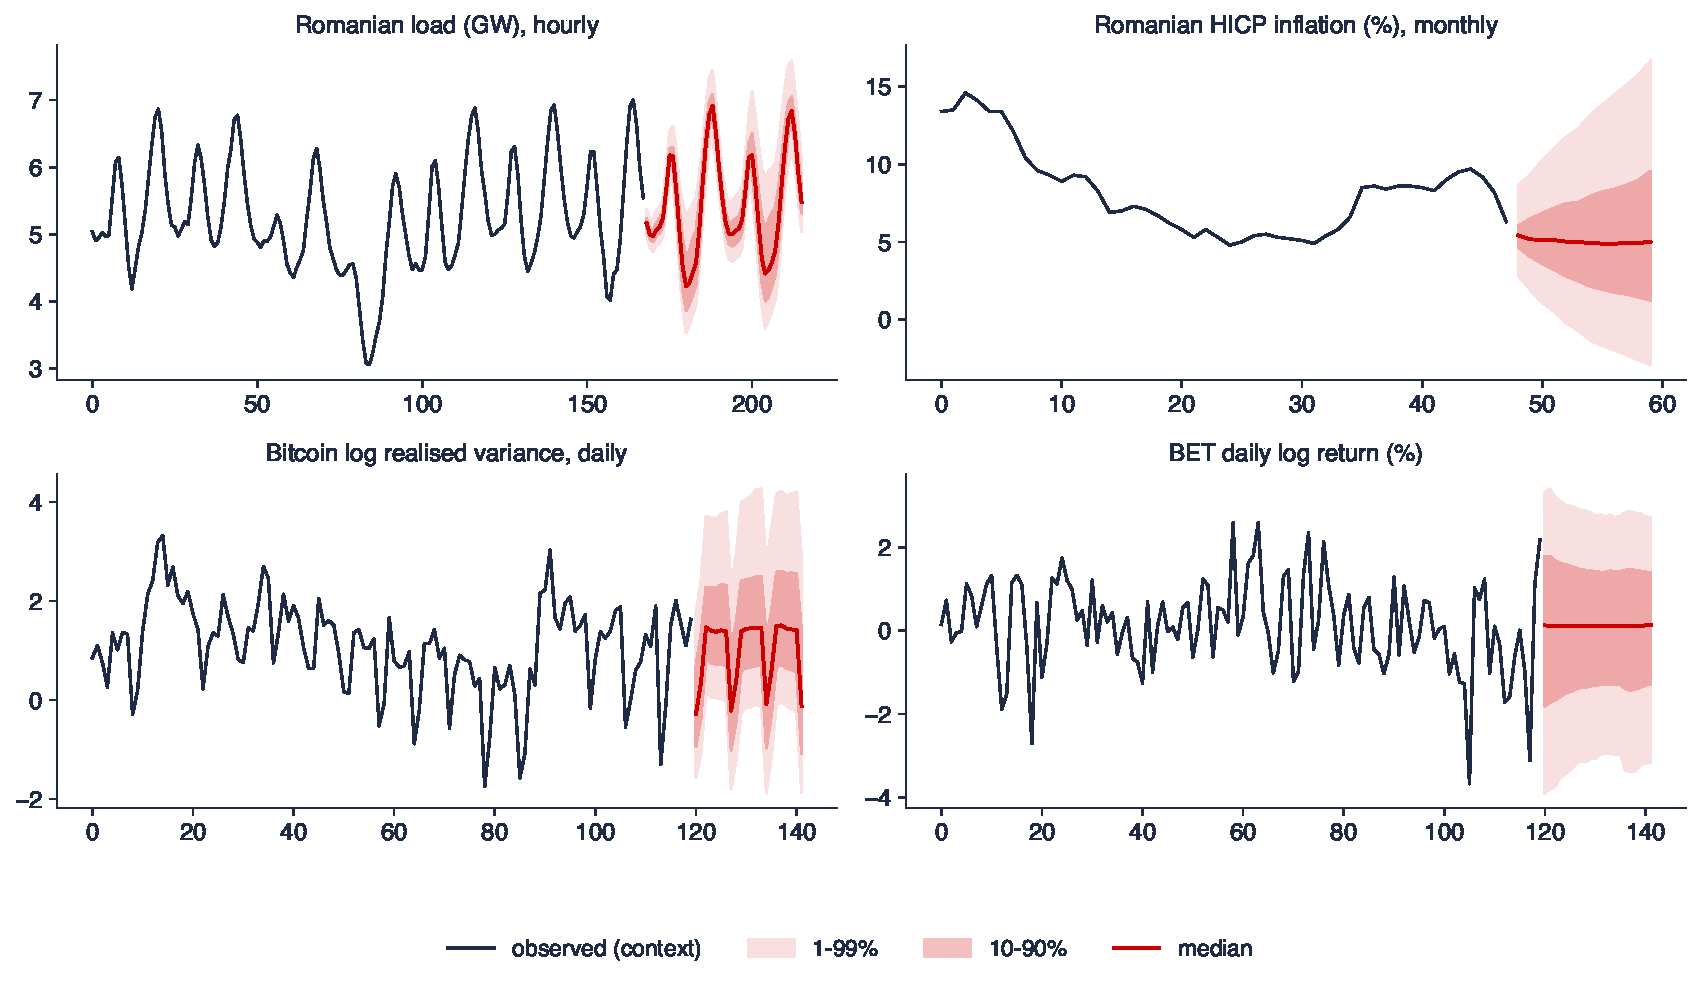
\includegraphics[width=0.97\textwidth,height=0.55\textheight,keepaspectratio]{ats_ch13_zeroshot.pdf}
\end{center}
\vspace{-0.25cm}
\begin{itemize}
    \item Chronos-2 de la ultima origine a fiecărui set de date: consumul României (48 de ore), inflația HICP a României (12 luni), logaritmul varianței realizate Bitcoin și randamentele zilnice BET (22 de zile); benzi 10--90\% și 1--99\%
\end{itemize}
\quantlet{ATS\_ch13\_zero\_shot}{\qlurl{ATS_ch13_zero_shot}}
\end{frame}

\begin{frame}{Interpretarea celor patru prognoze}
\itemsize{\small}
\begin{itemize}
    \item Consumul: formele zilnice și săptămînale sînt continuate cu benzi înguste: transferul de formă în cel mai bun caz
    \item Inflația: o traiectorie netedă spre nivelul recent, cu benzi care se lărgesc cu orizontul: aproape de ce ar da un model AR persistent
    \item Log RV pentru Bitcoin: un tipar săptămînal (varianță mai mică la sfîrșit de săptămînă) în jurul unui nivel stabilit de context; randamentele: o mediană constantă și o bandă simetrică, adică o distribuție necondiționată
    \item Benzile randamentelor din cuantilele de 1\% și 99\%: VaR 1\% Chronos-2 pentru ziua următoare este 3{,}90 (\% din valoare); secțiunea 8 verifică dacă astfel de cifre sînt calibrate
\end{itemize}
\end{frame}

\begin{frame}{Recapitulare: familiile de modele}
\itemsize{\small}
\begin{itemize}
    \item Familiile diferă prin intrare (token-uri, patch-uri, decalaje), arhitectură (encoder, decoder, recurentă) și ieșire (categorială, cuantile, parametrică)
    \item Domeniul cuantilelor este o constrîngere de proiectare: doar decile, cu excepția Chronos-2
    \item Zero-shot este varianta implicită; covariabilele în context și învățarea încrucișată sînt noile pîrghii; API-urile închise nu pot fi verificate
\end{itemize}
\end{frame}


%=============================================================================
\section{Benchmark-uri, contaminare și testare}
%=============================================================================

\begin{frame}{Benchmark-uri pentru modelele preantrenate}
\itemsize{\small}
\begin{itemize}
    \item \textbf{GIFT-Eval} \refAks: 23 de seturi de date, peste 144\,000 de serii, 177 de milioane de puncte, șapte domenii, zece frecvențe, orizonturi scurte și lungi; un set de preantrenare fără scurgere
    \item \textbf{fev-bench} \refShc: 100 de sarcini în șapte domenii, 46 cu covariabile; rate de cîștig și scoruri de abilitate cu intervale de încredere bootstrap
    \item \textbf{Benchmark-uri live}: prognoze înregistrate înainte să existe rezultatele, de exemplu TS-Arena \refMey{} și Impermanent \refGarB: singurul design imun la contaminare prin construcție
    \item Repere clasice pentru ce cere o comparație corectă: M5 \refMak; capcanele catalogate de \refHAB
\end{itemize}
\end{frame}

\begin{frame}{Agregarea scorurilor pe mai multe serii}
\itemsize{\small}
\begin{itemize}
    \item Scoruri fără scală: MASE $= \frac{1}{H}\sum_h|y_{T+h} - \hat y_{T+h}| \big/ \frac{1}{T-m}\sum_t|y_t - y_{t-m}|$ \refHK; WQL $= 2\sum_{t,\tau}\rho_\tau(y_t - \hat q_{\tau,t})\big/\sum_t|y_t|$
    \begin{itemize}
        \item $\rho_\tau(u) = u(\tau - \mathbf 1\{u < 0\})$ (pinball); media pe $\tau$ aproximează CRPS (\atschlink{https://danpele.github.io/Advanced-Time-Series/RO/Cursuri/capitol1_evaluarea_prognozelor.pdf}{Capitolul 1})
    \end{itemize}
    \item Scorurile relative $r_s = L_s(\text{model})/L_s(\text{referință})$ se combină prin \textbf{media geometrică} \refFW: clasamentele nu depind de alegerea modelului de referință, iar cîștigurile și pierderile sînt tratate simetric
    \begin{itemize}
        \item scorul de abilitate $1 - \bar r_{\mathrm{geo}}$; rata de cîștig: ponderea seriilor pe care un model îl întrece pe altul
    \end{itemize}
    \item Media aritmetică a rapoartelor recompensează seriile slabe ale modelului de referință; media erorilor brute este dominată de seria cu scala cea mai mare
\end{itemize}
\end{frame}

\begin{frame}{Scurgerea de informație și contaminarea}
\itemsize{\small}
\begin{itemize}
    \item \textbf{Scurgerea seriilor}: o serie de evaluare (sau o copie apropiată) se află în corpusul de preantrenare; Chronos separă din acest motiv rezultatele în domeniu (Benchmark I) de cele zero-shot (Benchmark II) \refAns
    \item \textbf{Contaminarea temporală}: fereastra de test precede data-limită a antrenării; modelul poate să fi văzut rezultatele altor serii, corelate, din aceeași perioadă
    \begin{itemize}
        \item LLM-urile reproduc valori economice exacte din perioada dinaintea datei-limită \refLTZ; un design cu două seturi de date împotriva contaminării, pentru prețurile electricității \refPE
    \end{itemize}
    \item Designuri care ajută
    \begin{itemize}
        \item evaluați doar după lansarea (sau data-limită declarată) a fiecărui model din comparație; folosim 1 noiembrie 2025, după ultimul dintre modelele noastre (Chronos-2, 30 octombrie 2025)
        \item comparați abilitatea relativă înainte și după: o scădere mare după lansare este un semnal de alarmă
        \item preînregistrați originile, orizonturile, metricile și modelele de referință înainte de a vedea rezultatele
    \end{itemize}
\end{itemize}
\end{frame}

\begin{frame}{Testarea pe multe serii}
\itemsize{\small}
\begin{itemize}
    \item O serie: DM cu corecția HLN \refDM, \refHLN; capacitatea condiționată \refGW; multe modele: MCS \refHLNa{} (toate în \atschlink{https://danpele.github.io/Advanced-Time-Series/RO/Cursuri/capitol1_evaluarea_prognozelor.pdf}{Capitolul 1})
    \item $S$ serii testate separat: la 5\% fiecare, sub ipoteza nulă se așteaptă aproximativ $0{,}05S$ respingeri false
    \begin{itemize}
        \item \textbf{Holm} \refHol{} (FWER): ordonați $p_{(1)} \le \dots \le p_{(S)}$, respingeți cît timp $p_{(k)} \le \alpha/(S - k + 1)$
        \item \textbf{Benjamini--Hochberg} \refBH{} (FDR): respingeți cele mai mici $k^*$, $k^* = \max\{k: p_{(k)} \le k\alpha/S\}$; valid sub independență sau dependență pozitivă
    \end{itemize}
    \item Teste agregate: mediați diferența de pierdere pe serii la fiecare origine, apoi un singur test DM cu varianță HAC: corelația dintre serii este păstrată în dimensiunea timpului
    \item Ranguri pe multe seturi de date: testele Friedman și Nemenyi \refDem; ele ignoră mărimea diferențelor și presupun seturi de date independente
\end{itemize}
\end{frame}

\begin{frame}{Recapitulare: benchmark-urile și testarea}
\itemsize{\small}
\begin{itemize}
    \item Agregați scoruri relative fără scală prin medii geometrice și raportați incertitudinea pe serii
    \item Contaminarea este o proprietate a perechii (model, fereastră de test): evaluați după lansare sau live
    \item Multe serii înseamnă multe teste: corectați cu Holm sau BH sau agregați înainte de testare
\end{itemize}
\end{frame}


%=============================================================================
\section{Dovezi pe datele noastre}
%=============================================================================

\begin{frame}{Designul comparațiilor noastre}
\itemsize{\small}
\begin{itemize}
    \item \textbf{Consumul României}: pentru ziua următoare, 24 de ore, în fiecare zi de la 1 ianuarie 2025 la 30 septembrie 2026 (638 de zile); context de 2048 de ore pentru foundation models
    \begin{itemize}
        \item modele de referință: naiv săptămînal; modelul ARX expert al lui \refZW{} pentru fiecare oră (\atschlink{https://danpele.github.io/Advanced-Time-Series/RO/Cursuri/capitol1_evaluarea_prognozelor.pdf}{Capitolul 1}); DLinear \refZen{} și N-BEATS \refOre{} antrenate global (\atschlink{https://danpele.github.io/Advanced-Time-Series/RO/Cursuri/capitol12_machine_learning_deep_learning.pdf}{Capitolul 12})
    \end{itemize}
    \item \textbf{Inflația UE}: 27 de țări, origini lunare mobile ianuarie 2012 -- august 2025, $h = 1, \dots, 12$; mers aleator, AR($p$) după AIC, ETS amortizat \refHKSG, DLinear și N-BEATS antrenate pe panel
    \item \textbf{Varianța realizată}: o zi înainte, log RV; HAR \refCor{} pe o fereastră mobilă de 1000 de zile; QLIKE \refPat
    \item Foundation models: Chronos-Bolt small, Chronos-2, TimesFM 2.5, TiRex, zero-shot, pe un CPU; Moirai și Lag-Llama nu au fost rulate (bibliotecile lor cer versiuni software mai vechi)
\end{itemize}
\end{frame}

\begin{frame}{Consumul României: acuratețea pentru ziua următoare}
\itemsize{\footnotesize}
\begin{center}
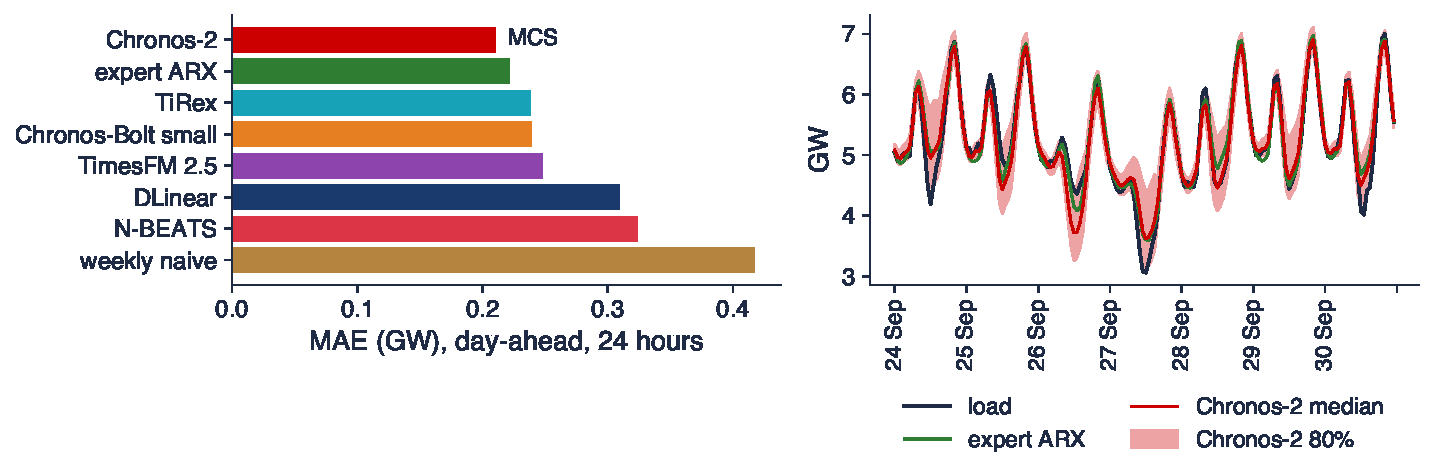
\includegraphics[width=0.97\textwidth,height=0.5\textheight,keepaspectratio]{ats_ch13_load.pdf}
\end{center}
\vspace{-0.25cm}
\begin{itemize}
    \item Stînga: MAE (GW) pe 24 de ore și 638 de zile, modelele din MCS de 10\% marcate; dreapta: ultima săptămînă din eșantion, ARX expert și Chronos-2 cu banda lui de 80\%
\end{itemize}
\quantlet{ATS\_ch13\_zero\_shot}{\qlurl{ATS_ch13_zero_shot}}
\end{frame}

\begin{frame}{Interpretarea comparației pentru consum}
\itemsize{\small}
\begin{itemize}
    \item MAE: Chronos-2 0{,}210, ARX expert 0{,}221, TiRex 0{,}238, Chronos-Bolt 0{,}239, TimesFM 0{,}248; DLinear 0{,}311, N-BEATS 0{,}325, naiv săptămînal 0{,}417 GW
    \item DM față de ARX expert: Chronos-2 $t = \ensuremath{-}3{,}05$ ($p$ = 0{,}002); celelalte trei foundation models sînt semnificativ mai slabe; MCS de 10\% este \{Chronos-2\}
    \item Acoperirea intervalului de 80\%: Chronos-2 75{,}5\%, Chronos-Bolt 81{,}2\%, TimesFM 81{,}2\%, ARX expert 78{,}1\%: niciunul nu este departe, niciunul nu este exact
    \item Un model univariat zero-shot egalează un model de domeniu consacrat pe o serie cu forme puternice și regulate; modelele deep globale antrenate pe trei ani pierd în fața ambelor
\end{itemize}
\end{frame}

\begin{frame}{Covariabile în context: calendarul și temperatura}
\itemsize{\footnotesize}
\begin{center}
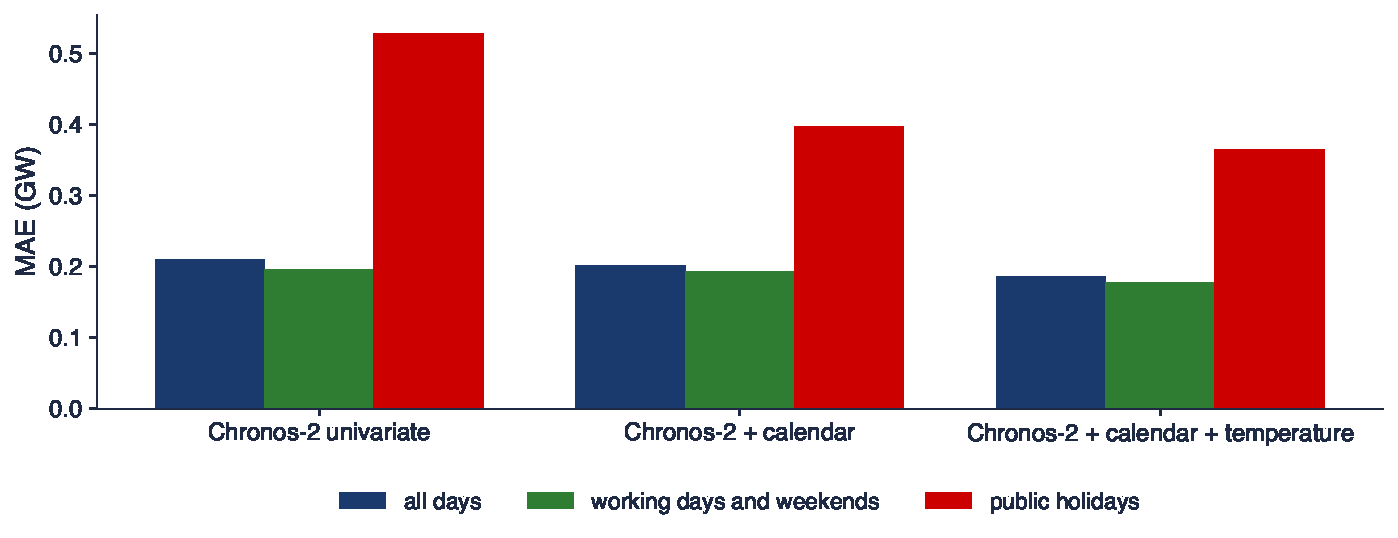
\includegraphics[width=0.97\textwidth,height=0.5\textheight,keepaspectratio]{ats_ch13_covariates.pdf}
\end{center}
\vspace{-0.25cm}
\begin{itemize}
    \item MAE Chronos-2 pe toate zilele, pe zilele obișnuite și pe cele 29 de zile de sărbătoare legală: univariat, cu indicatori de weekend și de sărbătoare și cu indicatori plus temperatura orară la București (valorile realizate pentru ziua prognozată: o limită superioară)
\end{itemize}
\quantlet{ATS\_ch13\_zero\_shot}{\qlurl{ATS_ch13_zero_shot}}
\end{frame}

\begin{frame}{Interpretarea experimentului cu covariabile}
\itemsize{\small}
\begin{itemize}
    \item Sărbători: MAE 0{,}527 univariat, 0{,}396 cu calendarul, 0{,}365 cu temperatura; zile obișnuite: 0{,}195; 0{,}193; 0{,}178
    \item Calendarul față de varianta univariată: DM $t = \ensuremath{-}2{,}79$ ($p$ = 0{,}005); temperatura în plus: $t = \ensuremath{-}7{,}02$ ($p$ $<$ 0{,}001)
    \item Efectul sărbătorilor este învățat în context din cîteva sărbători anterioare aflate în fereastra de 2048 de ore; niciun parametru nu a fost estimat
    \item Temperatura realizată nu este disponibilă la origine: un test operațional cere prognoze meteo arhivate
\end{itemize}
\end{frame}

\begin{frame}{Inflația UE: 27 de țări, 12 orizonturi}
\itemsize{\footnotesize}
\begin{center}
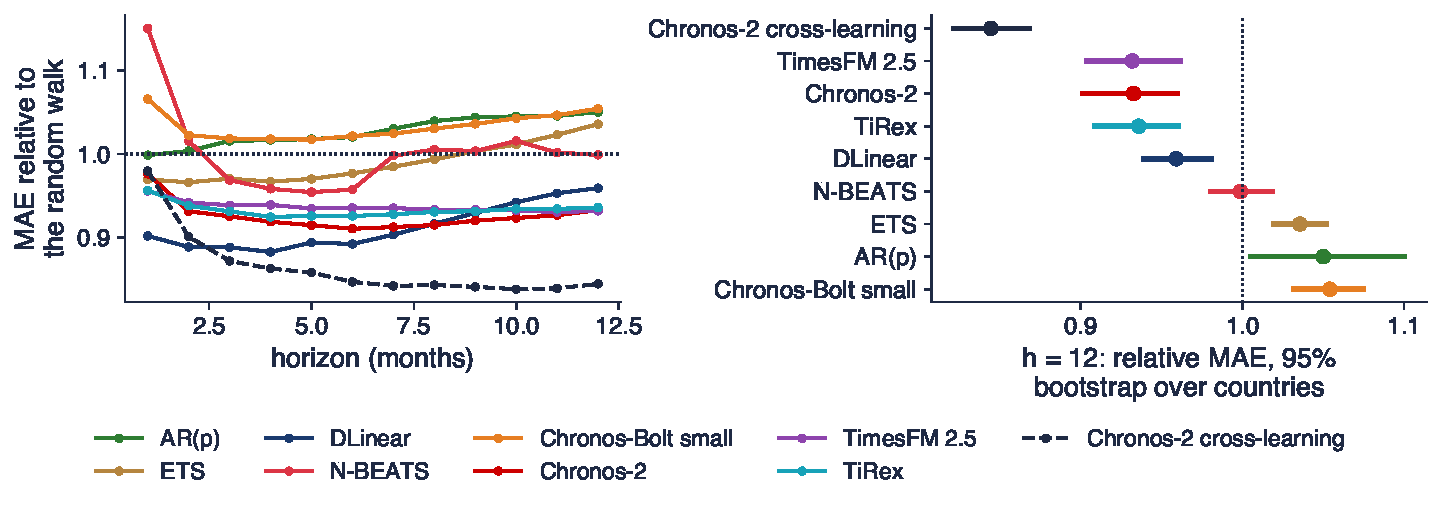
\includegraphics[width=0.97\textwidth,height=0.5\textheight,keepaspectratio]{ats_ch13_inflation.pdf}
\end{center}
\vspace{-0.25cm}
\begin{itemize}
    \item Stînga: MAE relativ la mersul aleator pe orizonturi, medie geometrică pe țări; dreapta: $h = 12$ cu intervale bootstrap de 95\% pe țări; origini ianuarie 2012 -- august 2025
\end{itemize}
\quantlet{ATS\_ch13\_benchmark}{\qlurl{ATS_ch13_benchmark}}
\end{frame}

\begin{frame}{Interpretarea panelului de inflație}
\itemsize{\small}
\begin{itemize}
    \item $h = 1$: AR 0{,}999, Chronos-2 0{,}976, TimesFM 0{,}956, TiRex 0{,}956; $h = 12$: AR 1{,}050, ETS 1{,}036, Chronos-2 0{,}933, TimesFM 0{,}932, TiRex 0{,}936, Bolt 1{,}054
    \item Modelele deep globale la $h = 12$: DLinear 0{,}959, N-BEATS 0{,}999; Chronos-2 cu învățare încrucișată pe cele 27 de țări: 0{,}845
    \item CRPS relativ la AR (medie geometrică pe țări): Chronos-2 0{,}860, TimesFM 0{,}875, TiRex 0{,}865, ETS 0{,}972
    \item Creșterea din 2021--2023 domină orice medie: nicio metodă univariată nu a anticipat-o, deci diferențele țin de viteza de adaptare, nu de anticipare
\end{itemize}
\end{frame}

\begin{frame}{România: prognoze din trei origini}
\itemsize{\footnotesize}
\begin{center}
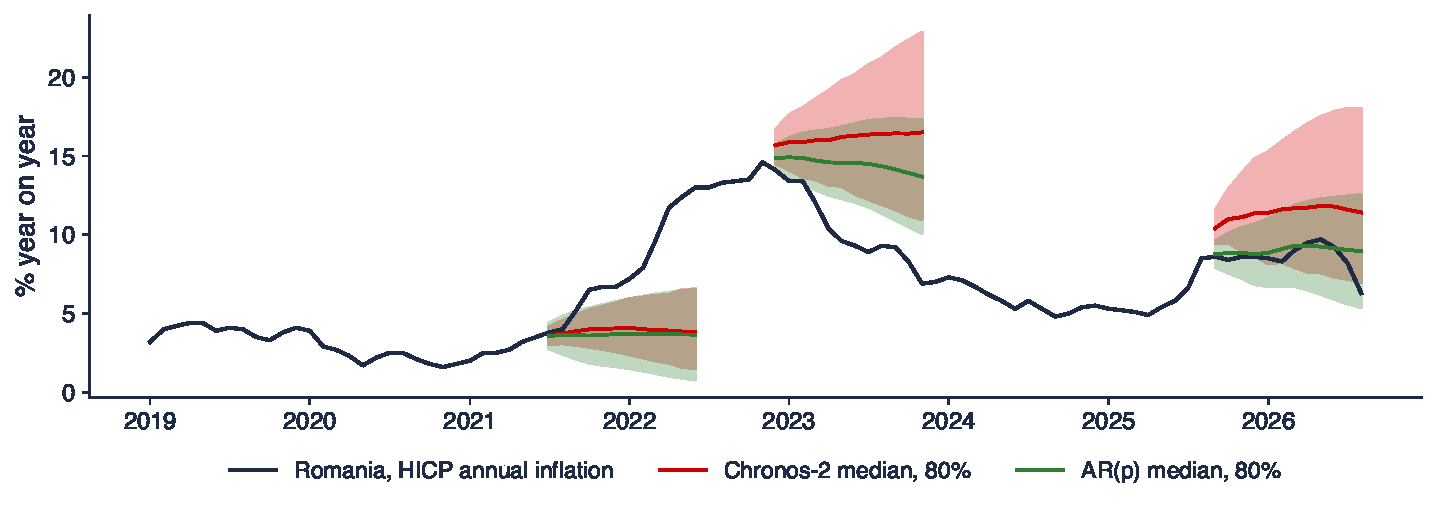
\includegraphics[width=0.97\textwidth,height=0.5\textheight,keepaspectratio]{ats_ch13_ro_inflation.pdf}
\end{center}
\vspace{-0.25cm}
\begin{itemize}
    \item Inflația anuală HICP a României și prognoze pe 12 luni cu benzi de 80\% din Chronos-2 și AR($p$), de la iunie 2021, noiembrie 2022 și august 2025
\end{itemize}
\quantlet{ATS\_ch13\_benchmark}{\qlurl{ATS_ch13_benchmark}}
\end{frame}

\begin{frame}{Interpretarea traiectoriilor pentru România}
\itemsize{\small}
\begin{itemize}
    \item De la iunie 2021: după 12 luni inflația a fost 13{,}0\%; mediana Chronos-2 3{,}8\% (80\%: 1{,}5 -- 6{,}6), AR 3{,}7\%
    \item De la noiembrie 2022, aproape de vîrf (14{,}6\% în noiembrie 2022): rezultat 6{,}9\%; Chronos-2 16{,}5\%, AR 13{,}7\%
    \item De la august 2025: rezultat 6{,}3\%; Chronos-2 11{,}4\%, AR 9{,}0\%; ultima observație este 6{,}3\% (august 2026)
    \item Ambele metode extrapolează persistența; punctele de întoarcere vin din informații din afara seriei (prețurile energiei, sfîrșitul plafonării prețurilor, majorarea TVA din august 2025, al cărei efect asupra inflației anuale durează exact 12 luni): cunoscute dinainte, deci covariabile naturale
\end{itemize}
\end{frame}

\begin{frame}{Douăzeci și șapte de teste deodată}
\itemsize{\footnotesize}
\begin{center}
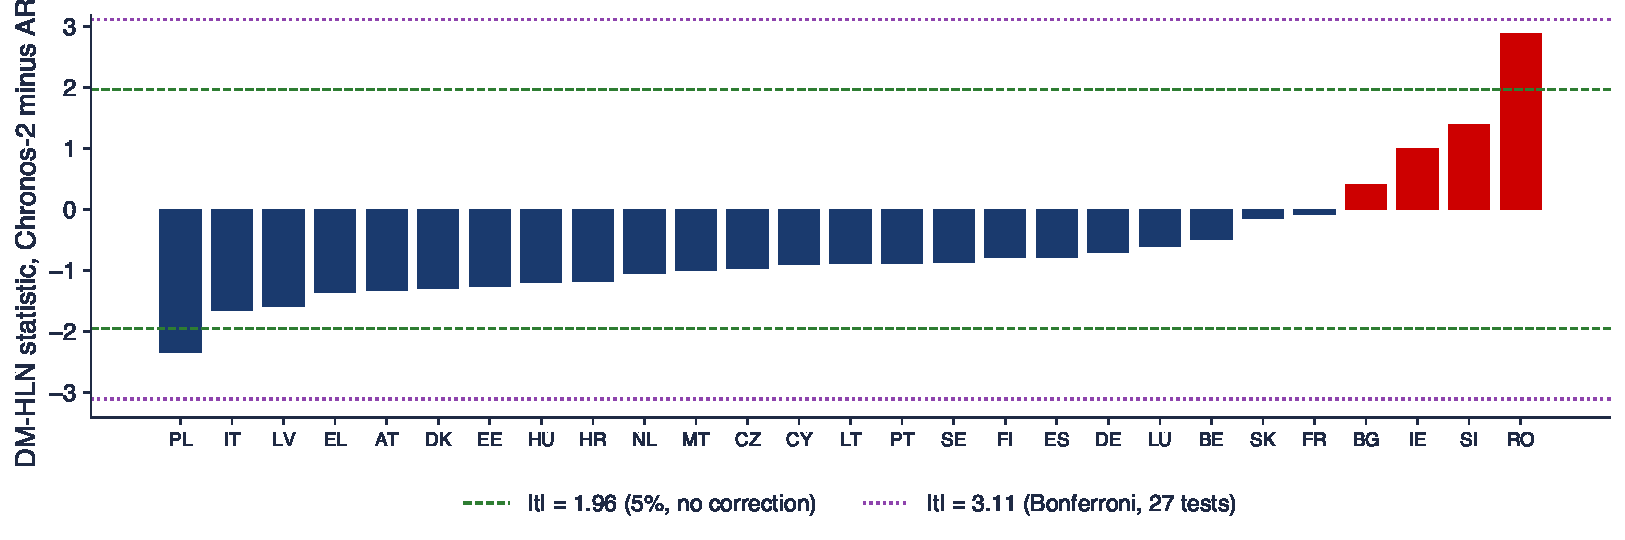
\includegraphics[width=0.97\textwidth,height=0.48\textheight,keepaspectratio]{ats_ch13_multiple.pdf}
\end{center}
\vspace{-0.25cm}
\begin{itemize}
    \item Statisticile DM--HLN pe țări (HAC cu $h - 1$ decalaje) ale erorilor absolute Chronos-2 minus AR($p$) la $h = 12$; negativ: Chronos-2 este mai bun
\end{itemize}
\quantlet{ATS\_ch13\_benchmark}{\qlurl{ATS_ch13_benchmark}}
\end{frame}

\begin{frame}{Interpretarea testelor multiple}
\itemsize{\small}
\begin{itemize}
    \item 23 din 27 de statistici sînt negative; 2 sînt semnificative la 5\% fără corecție (1 în favoarea Chronos-2, 1 în favoarea AR)
    \item Cu Holm: 0 respingeri; cu Benjamini--Hochberg: 0; România: $t = 2{,}88$, $p$ = 0{,}005
    \item Agregat pe cele 27 de țări (diferența medie de pierdere la fiecare origine, varianță HAC): $t = \ensuremath{-}1{,}35$, $p$ = 0{,}180; intervalele bootstrap din graficul anterior tratează țările ca independente și par mai precise decît sînt
    \item O lucrare care raportează țările în care modelul ei cîștigă la 5\% raportează zgomot; testul agregat și numerele ajustate pentru multiplicitate sînt rezumatul onest
\end{itemize}
\end{frame}

\begin{frame}{Varianța realizată: foundation models față de HAR}
\itemsize{\footnotesize}
\begin{center}
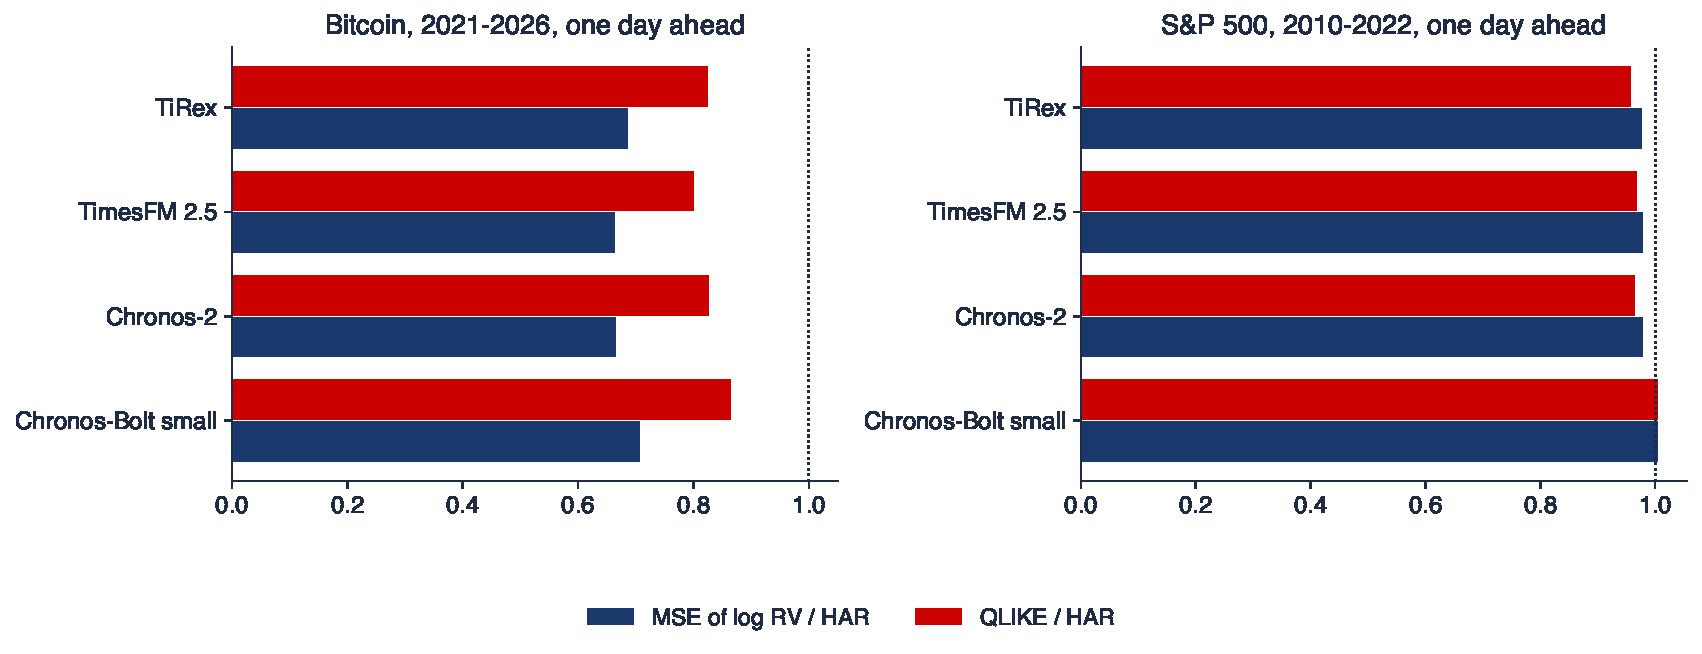
\includegraphics[width=0.97\textwidth,height=0.5\textheight,keepaspectratio]{ats_ch13_rv.pdf}
\end{center}
\vspace{-0.25cm}
\begin{itemize}
    \item Log RV pentru ziua următoare: MSE și QLIKE relativ la HAR; Bitcoin (Binance, 1 ianuarie 2021 -- 18 septembrie 2026, $n = 2\,084$), S\&P 500 (Oxford-Man, 4 ianuarie 2010 -- 25 februarie 2022, $n = 3\,047$)
\end{itemize}
\quantlet{ATS\_ch13\_benchmark}{\qlurl{ATS_ch13_benchmark}}
\end{frame}

\begin{frame}{Interpretarea comparației pentru volatilitate}
\itemsize{\small}
\begin{itemize}
    \item Bitcoin, QLIKE relativ la HAR: Chronos-2 0{,}825, TimesFM 0{,}800, TiRex 0{,}824, Bolt 0{,}864; MCS (10\%): \{Chronos-2, TimesFM 2.5, TiRex\}
    \item S\&P 500: Chronos-2 0{,}963, TimesFM 0{,}968, TiRex 0{,}956, Bolt 1{,}004; MCS (10\%): \{Chronos-2, TimesFM 2.5, TiRex\}
    \item Trei dintre cele patru modele zero-shot întrec HAR pe ambele active, iar HAR nu intră în niciun MCS: memoria lentă a lui log RV (\atschlink{https://danpele.github.io/Advanced-Time-Series/RO/Cursuri/capitol10_memorie_lunga_rough_volatility.pdf}{Capitolul 10}) este o formă pe care un corpus o poate preda; cîștigul este mare pentru Bitcoin și mic pentru S\&P 500
    \item Studii recente ajung la verdicte mixte \refGoe, \refBri, \refRNW: cîștigurile depind de activ, de orizont și de funcția de pierdere, iar fine-tuning-ul sau preantrenarea pe date financiare contează adesea
\end{itemize}
\end{frame}

\begin{frame}{Înainte și după lansări}
\itemsize{\footnotesize}
\begin{center}
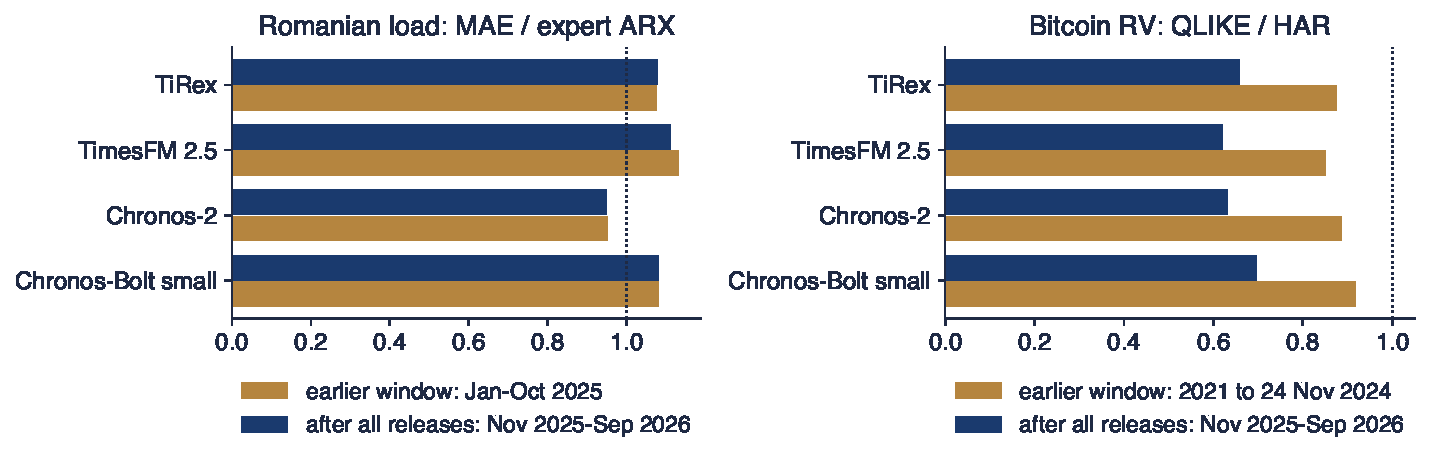
\includegraphics[width=0.97\textwidth,height=0.5\textheight,keepaspectratio]{ats_ch13_contamination.pdf}
\end{center}
\vspace{-0.25cm}
\begin{itemize}
    \item Pierderea relativă a fiecărui model într-o fereastră anterioară și în fereastra de după toate lansările (din 1 noiembrie 2025): consum (MAE / ARX expert) și Bitcoin (QLIKE / HAR)
\end{itemize}
\quantlet{ATS\_ch13\_benchmark}{\qlurl{ATS_ch13_benchmark}}
\end{frame}

\begin{frame}{Interpretarea verificării contaminării}
\itemsize{\small}
\begin{itemize}
    \item Consum, Chronos-2: 0{,}952 înainte, 0{,}950 după; TimesFM: 1{,}133; 1{,}112; fereastra anterioară (ianuarie--octombrie 2025) precede ambele lansări
    \item Bitcoin, Chronos-2: 0{,}886 (2021 -- 24 noiembrie 2024) și 0{,}631 (după); TiRex: 0{,}874; 0{,}658; ferestrele de după lansare au 334 și 322 de zile
    \item Nicio deteriorare după lansări (pentru Bitcoin rapoartele sînt chiar mai mici): nicio dovadă de contaminare aici; dar absența unei scăderi nu dovedește absența scurgerii, iar piețele se schimbă între ferestre
\end{itemize}
\end{frame}

\begin{frame}{Recapitulare: dovezile}
\itemsize{\small}
\begin{itemize}
    \item Forme puternice (consum): cel mai bun foundation model egalează sau întrece modelul de domeniu; forme slabe (randamente): puțin de transferat
    \item Inflația: înaintea modelelor AR și ETS în media panelului (cel mai mult cu învățarea încrucișată), dar nicio diferență pe țară nu rezistă corecțiilor Holm sau BH, iar testul agregat nu este semnificativ
    \item Varianța realizată: modelele zero-shot întrec HAR, clar pentru Bitcoin, la limită pentru S\&P 500
    \item Covariabilele în context ajută acolo unde calendarul contează; ferestrele de după lansare nu arată semne de contaminare
\end{itemize}
\end{frame}


%=============================================================================
\section{Modele de limbaj pentru serii de timp}
%=============================================================================

\begin{frame}{LLMTime: numerele ca text}
\itemsize{\small}
\begin{itemize}
    \item \refGru: se rescalează, se rotunjește la un număr fix de cifre, valorile se scriu ca cifre separate prin spații și virgule; un LLM obișnuit continuă șirul
    \begin{itemize}
        \item probabilitățile cifră cu cifră definesc o densitate ierarhică (pe mai multe intervale) pentru valori continue; eșantionarea repetată dă cuantile
    \end{itemize}
    \item Rezultatele lucrării: competitiv zero-shot pe unele benchmark-uri; tokenizarea numerelor contează (un model mai nou putea fi mai slab din cauza felului în care împarte cifrele); alinierea (RLHF) strică calibrarea
    \item Costuri: mii de token-uri pe serie și multe eșantioane pentru o prognoză; fereastra de context limitează istoria; LLM-ul poate să fi memorat datele
\end{itemize}
\end{frame}

\begin{frame}{Reprogramarea unui LLM înghețat}
\itemsize{\small}
\begin{itemize}
    \item \textbf{Time-LLM} \refJin: patch-urile seriei sînt proiectate pe prototipuri de text (embedding-uri de cuvinte), un prefix de prompt descrie sarcina și statisticile; LLM-ul rămîne înghețat, o proiecție citește prognoza
    \item \textbf{One Fits All} (GPT4TS) \refZho: un GPT-2 înghețat, cu embedding-ul de intrare, normalizările de strat și stratul de ieșire antrenate, pentru prognoză, clasificare și detectarea anomaliilor
    \item Afirmația: cunoașterea din limbaj se transferă la serii; testul afirmației este o ablație care elimină modelul de limbaj
\end{itemize}
\end{frame}

\begin{frame}{Studiu de caz: sînt modelele de limbaj chiar utile?}
\itemsize{\small}
\begin{columns}[T]
\begin{column}{0.56\textwidth}
\begin{itemize}
    \item \refTan: trei prognozatori pe bază de LLM (inclusiv Time-LLM și GPT4TS), aceleași benchmark-uri, trei ablații
    \item Ablațiile
    \begin{itemize}
        \item eliminarea LLM-ului; înlocuirea lui cu un strat de atenție; înlocuirea cu un bloc Transformer simplu
    \end{itemize}
    \item Rezultat: nicio degradare, adesea o îmbunătățire; LLM-urile preantrenate nu sînt mai bune decît același model antrenat de la zero, nu modelează dependența secvențială, nu ajută cînd datele sînt puține
    \item Antrenarea și inferența costă cu ordine de mărime mai mult
\end{itemize}
\end{column}
\begin{column}{0.42\textwidth}
\begin{itemize}
    \item Metoda contează mai mult decît rezultatul
    \item o afirmație despre arhitectură cere o ablație cu calcul și ajustare comparabile
    \item foundation models antrenate pe serii (Chronos, TimesFM, TiRex) nu sînt vizate de această critică; LLM-urile folosite ca prognozatori sînt
    \item LLM-urile rămîn utile în jurul prognozei: cod, literatură, critică (secțiunea 9)
\end{itemize}
\end{column}
\end{columns}
\end{frame}

\begin{frame}{Memorare și anticiparea viitorului}
\itemsize{\small}
\begin{itemize}
    \item \refLTZ: LLM-urile reproduc cu mare precizie valori macroeconomice și de piață din perioada lor de antrenare, chiar și cînd li se cere să nu folosească informații viitoare
    \begin{itemize}
        \item un backtest înainte de data-limită a antrenării măsoară memoria, nu capacitatea de prognoză
    \end{itemize}
    \item Pentru foundation models pe serii de timp, aceeași logică se aplică seriilor publice din corpus (electricitate, trafic, M4)
    \begin{itemize}
        \item dovezile noastre: ferestre de după toate lansările (secțiunea 4); cele mai puternice dovezi: prognoze live, preînregistrate
    \end{itemize}
    \item O regulă practică: precizați data-limită de antrenare a fiecărui model și începutul ferestrei de evaluare în același tabel
\end{itemize}
\end{frame}

\begin{frame}{Recapitulare: LLM}
\itemsize{\small}
\begin{itemize}
    \item LLMTime și reprogramarea arată că modelele de text pot fi adaptate la serii; ablațiile arată că partea de limbaj rareori este cea care ajută
    \item Memorarea face ca evaluarea prognozelor LLM înainte de data-limită să nu fie validă
\end{itemize}
\end{frame}


%=============================================================================
\section{Predicția conformală}
%=============================================================================

\begin{frame}{Originea predicției conformale}
\itemsize{\small}
\begin{columns}[T]
\begin{column}{0.42\textwidth}
\centering
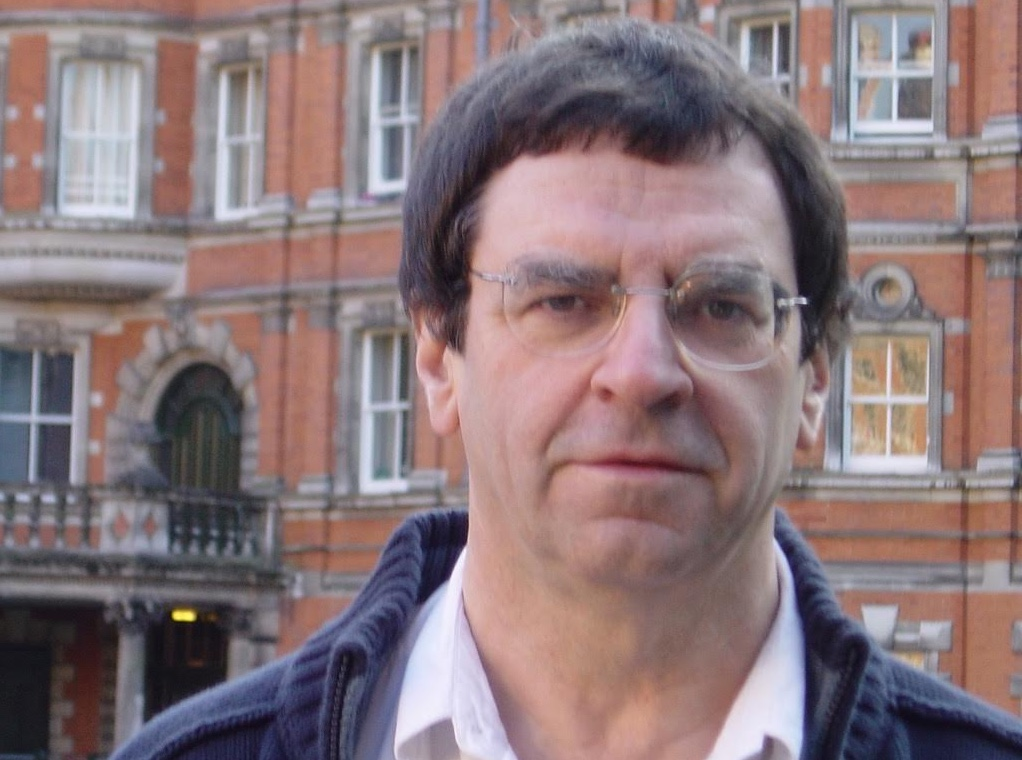
\includegraphics[height=0.36\textheight]{ch13_gammerman_2018.jpg}\\[1mm]
\imgcap{Alexander Gammerman, Royal Holloway, 2018}
\imgcredit{https://commons.wikimedia.org/wiki/File:Alexander-Gammerman-professor-at-RHUL.jpg}{Foto: Jaguar224 (2018); CC BY-SA 4.0; Wikimedia Commons}
\end{column}
\begin{column}{0.56\textwidth}
\begin{itemize}
    \item Vovk, Gammerman și Shafer \refVGS, \refVGSb: mulțimi de predicție valide în eșantioane finite doar sub interschimbabilitate, pentru orice model predictiv
    \item Ideea: cît de „conformă” este o valoare candidat cu datele văzute, măsurat printr-un rang
    \item Statistica modernă a adoptat-o ca înveliș în jurul metodelor de machine learning \refLei, \refAB
\end{itemize}
\end{column}
\end{columns}
\end{frame}

\begin{frame}{Interschimbabilitatea și garanția urmărită}
\itemsize{\small}
\begin{itemize}
    \item $Z_1, \dots, Z_{n+1}$, $Z_i = (X_i, Y_i)$, sînt \textbf{interschimbabile} dacă $(Z_{\pi(1)}, \dots, Z_{\pi(n+1)}) \overset{d}{=} (Z_1, \dots, Z_{n+1})$ pentru orice permutare $\pi$
    \begin{itemize}
        \item i.i.d.\ implică interschimbabilitate; extragerile fără întoarcere sînt interschimbabile, dar dependente; un AR(1) staționar nu este interschimbabil
    \end{itemize}
    \item \textbf{Acoperire marginală}: $\Pr\{Y_{n+1} \in \hat C(X_{n+1})\} \ge 1 - \alpha$, probabilitatea fiind luată împreună pe datele de calibrare și pe punctul de test
    \begin{itemize}
        \item nu acoperirea \textbf{condiționată} $\Pr\{Y \in \hat C(x) \mid X = x\} \ge 1 - \alpha$ pentru orice $x$ și nici acoperirea condiționată de eșantionul de calibrare
    \end{itemize}
    \item Un \textbf{scor de neconformitate} $s(x, y)$: mare cînd $y$ este neobișnuit dat fiind $x$, de exemplu $|y - \hat\mu(x)|$, $|y - \hat\mu(x)|/\hat\sigma(x)$ sau scorul CQR de mai jos
\end{itemize}
\end{frame}

\begin{frame}{Predicția split conformal}
\itemsize{\small}
\begin{itemize}
    \item Se estimează $\hat\mu$ pe un set de antrenare; se calculează $S_i = s(X_i, Y_i)$ pe $n$ puncte de calibrare \refPap, \refLei
    \begin{itemize}
        \item $\hat q = S_{(k)}$, $k = \lceil (n + 1)(1 - \alpha) \rceil$ (a $k$-a cea mai mică valoare; $+\infty$ dacă $k > n$); $\hat C(x) = \{y: s(x, y) \le \hat q\}$
    \end{itemize}
    \item \textbf{Teoremă}: dacă $(X_i, Y_i)_{i \le n+1}$ sînt interschimbabile, $\Pr\{Y_{n+1} \in \hat C(X_{n+1})\} \ge 1 - \alpha$; fără egalități, și $\le 1 - \alpha + 1/(n + 1)$
    \begin{itemize}
        \item demonstrație: dat fiind $\hat\mu$, scorurile $S_1, \dots, S_{n+1}$ sînt interschimbabile, deci rangul lui $S_{n+1}$ este uniform pe $\{1, \dots, n + 1\}$; $Y_{n+1} \in \hat C \iff$ rangul $\le k$, cu probabilitatea $k/(n + 1) \ge 1 - \alpha$ (\atsapplink{atsapp1}{atssrc1}{Anexă})
    \end{itemize}
    \item Nicio ipoteză asupra modelului sau a distribuției: un model slab dă intervale largi, nu invalide
\end{itemize}
\end{frame}

\begin{frame}{Acoperirea condiționată de setul de calibrare}
\itemsize{\footnotesize}
\begin{center}
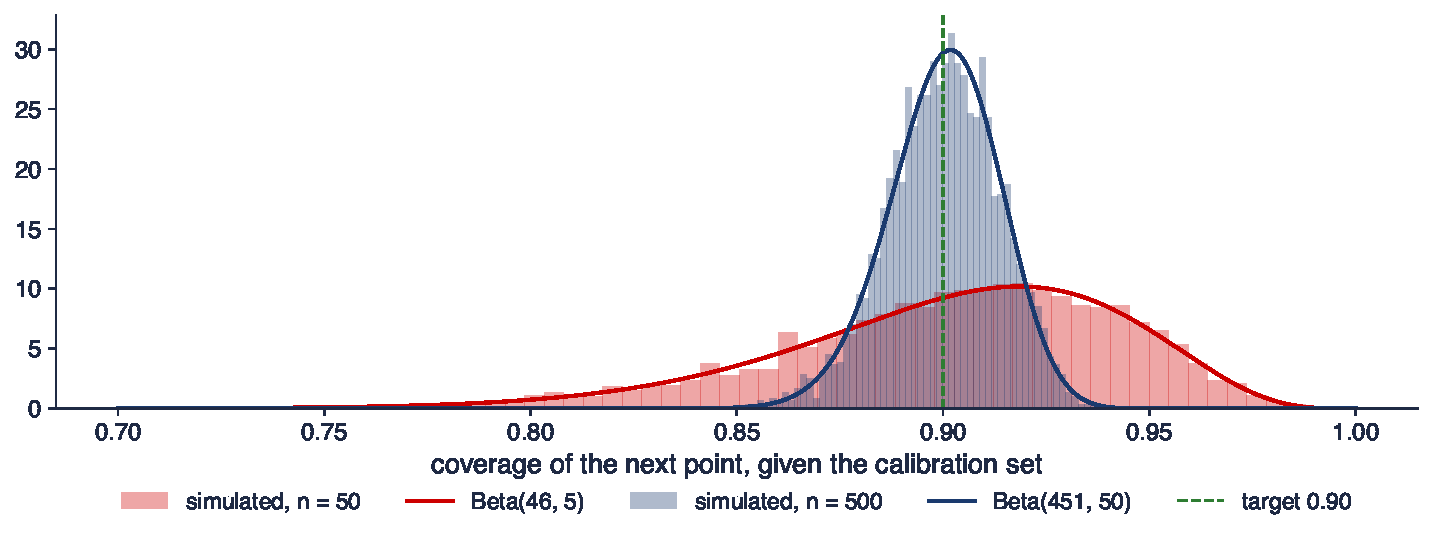
\includegraphics[width=0.97\textwidth,height=0.48\textheight,keepaspectratio]{ats_ch13_split_coverage.pdf}
\end{center}
\vspace{-0.25cm}
\begin{itemize}
    \item Acoperirea $F(\hat q)$ a punctului următor pentru 4000 de seturi de calibrare de $n = 50$ și $n = 500$ scoruri, $\alpha = 0{,}1$, și legea exactă Beta($k$, $n + 1 - k$)
\end{itemize}
\quantlet{ATS\_ch13\_conformal\_basics}{\qlurl{ATS_ch13_conformal_basics}}
\end{frame}

\begin{frame}{Interpretarea distribuției acoperirii}
\itemsize{\small}
\begin{itemize}
    \item Acoperirea medie 0{,}902 ($n = 50$) și 0{,}900 ($n = 500$), cum dă teoria (0{,}902; 0{,}900): garanția marginală este valabilă în medie pe seturile de calibrare
    \item Un set de calibrare este o singură extragere: abaterea standard 0{,}041 și 0{,}014; cu $n = 50$, 26\% dintre seturi dau acoperire sub 0,88, cu $n = 500$ doar 7\%
    \item Deoarece $F(\hat q) \sim$ Beta($k$, $n + 1 - k$), alegerea lui $n$ este un calcul de mărime a eșantionului: abaterea standard este aproximativ $\sqrt{\alpha(1 - \alpha)/n}$
\end{itemize}
\end{frame}

\begin{frame}{Regresia cuantilică conformalizată}
\itemsize{\small}
\begin{columns}[T]
\begin{column}{0.32\textwidth}
\centering

\includegraphics[height=0.34\textheight]{ch13_candes_2012.jpg}\\[1mm]
\imgcap{Emmanuel Candès, 2012}
\imgcredit{https://commons.wikimedia.org/wiki/File:Emmanuel_Cand\%C3\%A8s.jpg}{Foto: Renate Schmid, MFO (2012); CC BY-SA 2.0 de; Wikimedia Commons}
\end{column}
\begin{column}{0.66\textwidth}
\begin{itemize}
    \item \refRPC: se estimează regresii cuantilice \refKB{} $\hat q_{\alpha/2}(x)$, $\hat q_{1-\alpha/2}(x)$ pe setul de antrenare
    \item Scorul $s(x, y) = \max\{\hat q_{\alpha/2}(x) - y,\; y - \hat q_{1-\alpha/2}(x)\}$: negativ în interiorul benzii
    \item $\hat C(x) = [\hat q_{\alpha/2}(x) - \hat q,\; \hat q_{1-\alpha/2}(x) + \hat q]$: banda este deplasată spre exterior (sau spre interior dacă $\hat q < 0$)
    \item Acoperirea marginală rezultă din teorema split; lățimea se adaptează la heteroscedasticitate prin modelele cuantilice
    \item Același scor calibrează cuantilele oricărui foundation model (secțiunea 8)
\end{itemize}
\end{column}
\end{columns}
\end{frame}

\begin{frame}{CQR pe designul lui Romano, Patterson și Candès}
\itemsize{\footnotesize}
\begin{center}
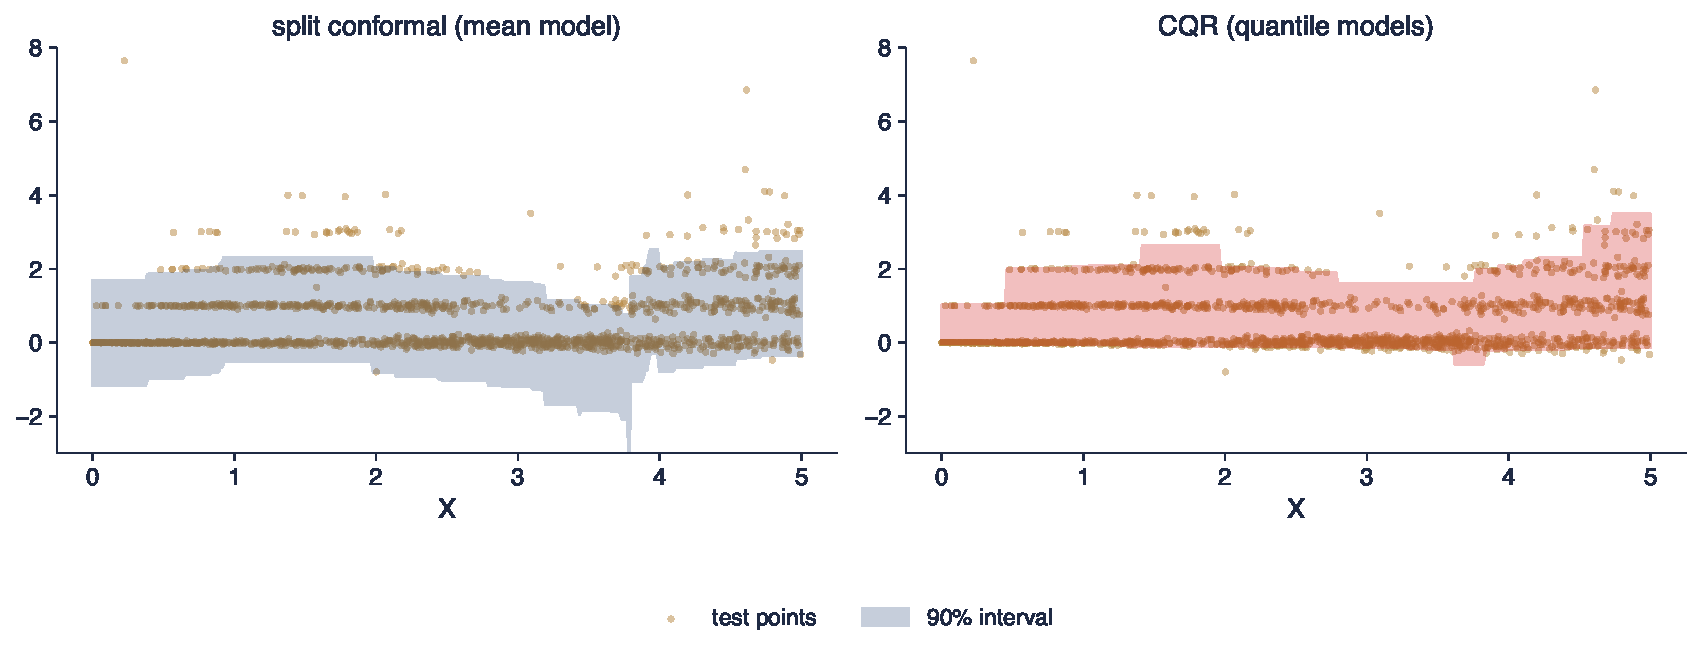
\includegraphics[width=0.97\textwidth,height=0.48\textheight,keepaspectratio]{ats_ch13_cqr.pdf}
\end{center}
\vspace{-0.25cm}
\begin{itemize}
    \item $Y = \mathrm{Pois}(\sin^2 X + 0{,}1) + 0{,}03X\varepsilon_1 + 25\cdot\mathbf 1\{U < 0{,}01\}\varepsilon_2$, $X \sim U[0, 5]$ (Figura 1 din lucrare); 1000 de puncte de antrenare și 1000 de calibrare; gradient boosting pentru medie și pentru cuantilele de 5\% și 95\%
\end{itemize}
\quantlet{ATS\_ch13\_conformal\_basics}{\qlurl{ATS_ch13_conformal_basics}}
\end{frame}

\begin{frame}{Interpretarea CQR}
\itemsize{\small}
\begin{itemize}
    \item Acoperirea pe datele de test: split conformal 0{,}918, CQR 0{,}915, modelele cuantilice brute 0{,}883; lățimea medie 2{,}84; 2{,}20 și 2{,}17
    \item Regresiile cuantilice brute acoperă prea puțin; CQR le repară aproape fără lățime suplimentară, în timp ce banda split de lățime constantă este cu 29\% mai largă
    \item Pe intervale ale lui $X$, ambele rămîn la cîteva puncte de 90\% (cele mai slabe intervale: CQR 0{,}892, split 0{,}896); cîștigul CQR este în lățime: îngust acolo unde $Y$ este concentrat, larg acolo unde zgomotul Poisson este mare
\end{itemize}
\end{frame}

\begin{frame}{Limitele acoperirii condiționate}
\itemsize{\small}
\begin{itemize}
    \item \textbf{Imposibilitate} \refVov, \refLW, \refBarB: dacă $\hat C$ are acoperire condiționată $\ge 1 - \alpha$ în aproape orice $x$, pentru orice distribuție cu $X$ continuu, atunci lungimea lui așteptată este infinită
    \begin{itemize}
        \item nicio metodă nu poate certifica în eșantioane finite acoperirea în fiecare punct al unei covariabile continue fără ipoteze
    \end{itemize}
    \item Rezultate posibile: acoperire în cadrul unui număr finit de grupuri (conformal Mondrian: calibrare separată pe grupuri); acoperire condiționată aproximativă sub ipoteze de netezime; acoperire condiționată de setul de calibrare cu probabilitate mare (legea Beta)
    \item Pentru serii de timp, condiția relevantă este trecutul: $\Pr\{Y_t \in \hat C_t \mid \mathcal F_{t-1}\}$; un backtest VaR (\atschlink{https://danpele.github.io/Advanced-Time-Series/RO/Cursuri/capitol9_var_es_backtesting.pdf}{Capitolul 9}) testează exact această proprietate pentru mulțimi unilaterale
\end{itemize}
\end{frame}

\begin{frame}{Recapitulare: predicția conformală}
\itemsize{\small}
\begin{itemize}
    \item Split conformal: un argument de rang dă acoperire marginală în eșantioane finite sub interschimbabilitate, pentru orice model
    \item CQR adaugă adaptivitate; mărimea eșantionului de calibrare controlează variabilitatea acoperirii realizate
    \item Acoperirea condiționată este imposibilă în general: testați-o, nu o afirmați
\end{itemize}
\end{frame}


%=============================================================================
\section{Predicția conformală pentru date dependente}
%=============================================================================

\begin{frame}{Interschimbabilitatea încălcată: rezultatele care rămîn valabile}
\itemsize{\small}
\begin{itemize}
    \item Seriile de timp încalcă interschimbabilitatea în trei feluri: dependența serială, volatilitatea variabilă, schimbările structurale; ultimele două strică cel mai mult acoperirea
    \item \textbf{Staționar și mixing}: split conformal rămîne aproximativ valid, cu o abatere a acoperirii controlată de coeficienții $\beta$-mixing și de mărimea calibrării \refOli
    \begin{itemize}
        \item permutările pe blocuri refac exactitatea sub condiții mai slabe \refCWZ
    \end{itemize}
    \item \textbf{Nestaționar}: nicio metodă statică nu poate funcționa; pragul trebuie să se miște odată cu datele: ponderi (Barber et al.), reestimare (EnbPI), reacție la erori (ACI, PID)
    \item Un cadru online comun: scorurile $S_t = s(X_t, Y_t)$ calculate din prognoze în afara eșantionului; la momentul $t$ se alege un prag $q_t$ din $S_1, \dots, S_{t-1}$; ratarea $\mathrm{err}_t = \mathbf 1\{S_t > q_t\}$
\end{itemize}
\end{frame}

\begin{frame}{Predicția conformală dincolo de interschimbabilitate}
\itemsize{\small}
\begin{itemize}
    \item \refBar: ponderi fixe $w_i \in [0, 1]$, alese înainte de a vedea datele; $\hat q$ = cuantila $(1 - \alpha)$ a lui $\sum_i \tilde w_i\delta_{S_i} + \tilde w_{n+1}\delta_{+\infty}$, $\tilde w_i = w_i/(1 + \sum_j w_j)$, $w_{n+1} = 1$
    \begin{itemize}
        \item \textbf{Teoremă}: acoperirea $\ge 1 - \alpha - \sum_i \tilde w_i\, d_{\mathrm{TV}}(Z, Z^i)$, unde $Z^i$ schimbă punctul de test cu punctul $i$
    \end{itemize}
    \item Sub interschimbabilitate abaterea este zero; sub o derivă lentă, $d_{\mathrm{TV}}$ este mic pentru punctele recente, deci ponderile geometrice $w_i = \rho^{n+1-i}$ o păstrează mică
    \begin{itemize}
        \item mărimea efectivă a eșantionului $\approx 1/(1 - \rho)$: $\rho = 0{,}99$ folosește aproximativ 100 de scoruri recente; robustețe în schimbul variabilității pragului
    \end{itemize}
    \item Schimbarea distribuției covariabilelor cu raport de verosimilitate cunoscut: ponderile $w(x) = dP_{\mathrm{test}}/dP_{\mathrm{train}}$ dau acoperire exactă \refTBCR
\end{itemize}
\end{frame}

\begin{frame}{Predicția conformală ponderată la puncte de schimbare}
\itemsize{\footnotesize}
\begin{center}
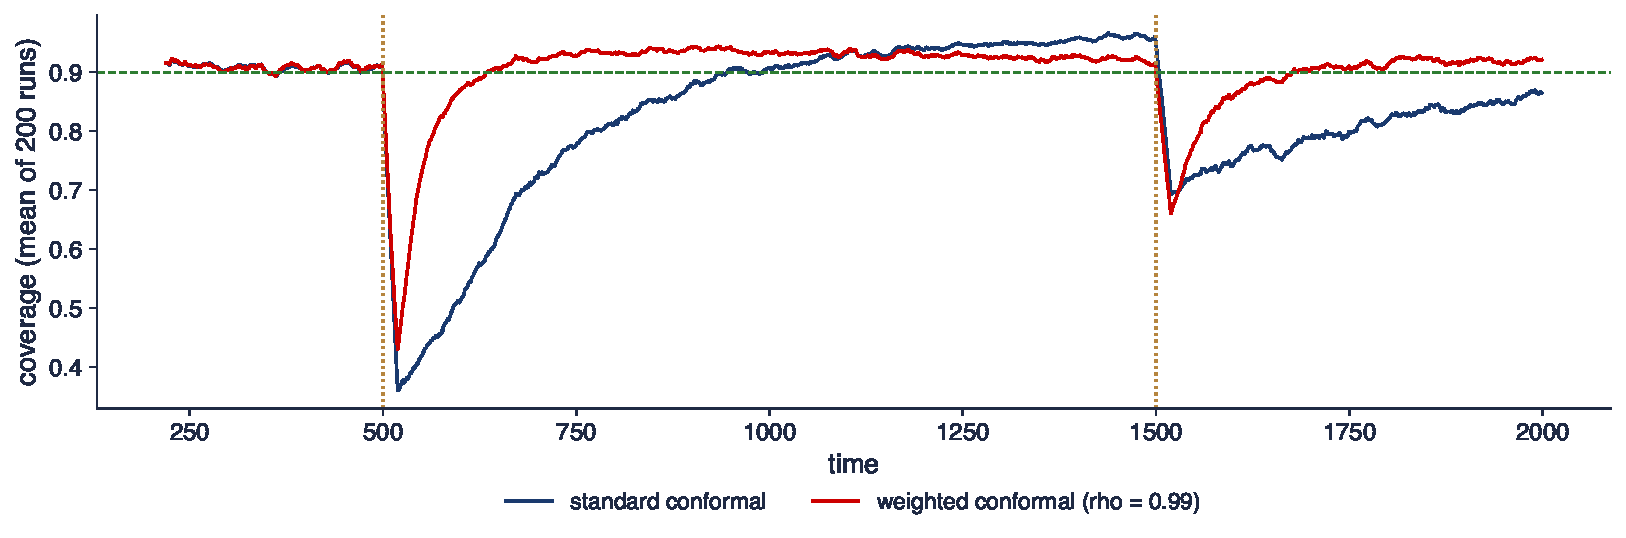
\includegraphics[width=0.97\textwidth,height=0.48\textheight,keepaspectratio]{ats_ch13_weighted.pdf}
\end{center}
\vspace{-0.25cm}
\begin{itemize}
    \item $Y_t = X_t'\beta_t + \varepsilon_t$, $X_t \sim N(0, I_4)$, $\beta$ se schimbă la $t = 500$ și $t = 1500$; cele mai mici pătrate pe toate datele trecute; reziduurile absolute prequential ca scoruri; acoperirea mediată pe 200 de rulări (medie mobilă pe 20 de pași)
\end{itemize}
\quantlet{ATS\_ch13\_conformal\_time}{\qlurl{ATS_ch13_conformal_time}}
\end{frame}

\begin{frame}{Interpretarea metodei ponderate}
\itemsize{\small}
\begin{itemize}
    \item Acoperirea medie după perioada inițială: standard 0{,}836, ponderat ($\rho = 0{,}99$) 0{,}900; cea mai slabă medie pe 20 de pași 0{,}36 față de 0{,}43
    \item Ambele se prăbușesc la o ruptură, pentru că estimarea prin cele mai mici pătrate este greșită o vreme; pragul ponderat uită scorurile vechi și își revine în aproximativ 100 de pași
    \item Prețul: lățimea medie 7{,}47 față de 6{,}22; garanția este o margine exprimată prin $d_{\mathrm{TV}}$, nu o acoperire exactă
\end{itemize}
\end{frame}

\begin{frame}{EnbPI: ansambluri fără împărțirea datelor}
\itemsize{\small}
\begin{itemize}
    \item \refXX, \refXXb: se estimează $B$ modele pe eșantioane bootstrap (pe blocuri, pentru a respecta dependența) ale perioadei de antrenare
    \begin{itemize}
        \item reziduuri leave-one-out: pentru punctul $i$ se agregă doar modelele al căror eșantion bootstrap l-a exclus pe $i$
        \item intervalul la $t$: $\hat f(x_t) \pm$ cuantila $(1 - \alpha)$ a ultimelor $T$ reziduuri absolute; după ce $y_t$ este observat, reziduul lui intră în fereastră, iar cel mai vechi iese
    \end{itemize}
    \item Fără reestimare la fiecare pas, fără împărțire pentru calibrare: eficient pe fluxuri lungi
    \item Garanția: acoperire asimptotică, condiționată, dacă erorile sînt staționare și puternic mixing, iar ansamblul este consistent; gîndit pentru serii de energie (solară și eoliană)
\end{itemize}
\end{frame}

\begin{frame}{Inferența conformală adaptivă}
\itemsize{\small}
\begin{itemize}
    \item \refGC: se folosește nivelul $\alpha_t$ la momentul $t$, $q_t$ = cuantila conformală $(1 - \alpha_t)$ a scorurilor recente, apoi $\alpha_{t+1} = \alpha_t + \gamma(\alpha - \mathrm{err}_t)$
    \begin{itemize}
        \item o ratare scade $\alpha_t$ (mulțimi mai largi); o acoperire îl crește; $\alpha_t \le 0$ dă $q_t = +\infty$ (toată dreapta), $\alpha_t \ge 1$ mulțimea vidă
    \end{itemize}
    \item \textbf{Teoremă}: pentru orice șir de date, $\Big|\frac1T\sum_{t=1}^T\mathrm{err}_t - \alpha\Big| \le \frac{\max\{\alpha_1, 1 - \alpha_1\} + \gamma}{\gamma T}$
    \begin{itemize}
        \item demonstrație: $\alpha_t$ rămîne în $[-\gamma, 1 + \gamma]$ și $\alpha_{T+1} - \alpha_1 = \gamma\sum_t(\alpha - \mathrm{err}_t)$; se împarte la $\gamma T$
    \end{itemize}
    \item Frecvență pe termen lung, nu acoperire condiționată: o medie rezistentă la orice adversar. Alegerea adaptivă a lui $\gamma$: AgACI \refZaf, DtACI \refGCb; ACI pentru VaR: \atschlink{https://danpele.github.io/Advanced-Time-Series/RO/Cursuri/capitol9_var_es_backtesting.pdf}{Capitolul 9}
\end{itemize}
\end{frame}

\begin{frame}{ACI pe volatilitatea bursieră}
\itemsize{\footnotesize}
\begin{center}
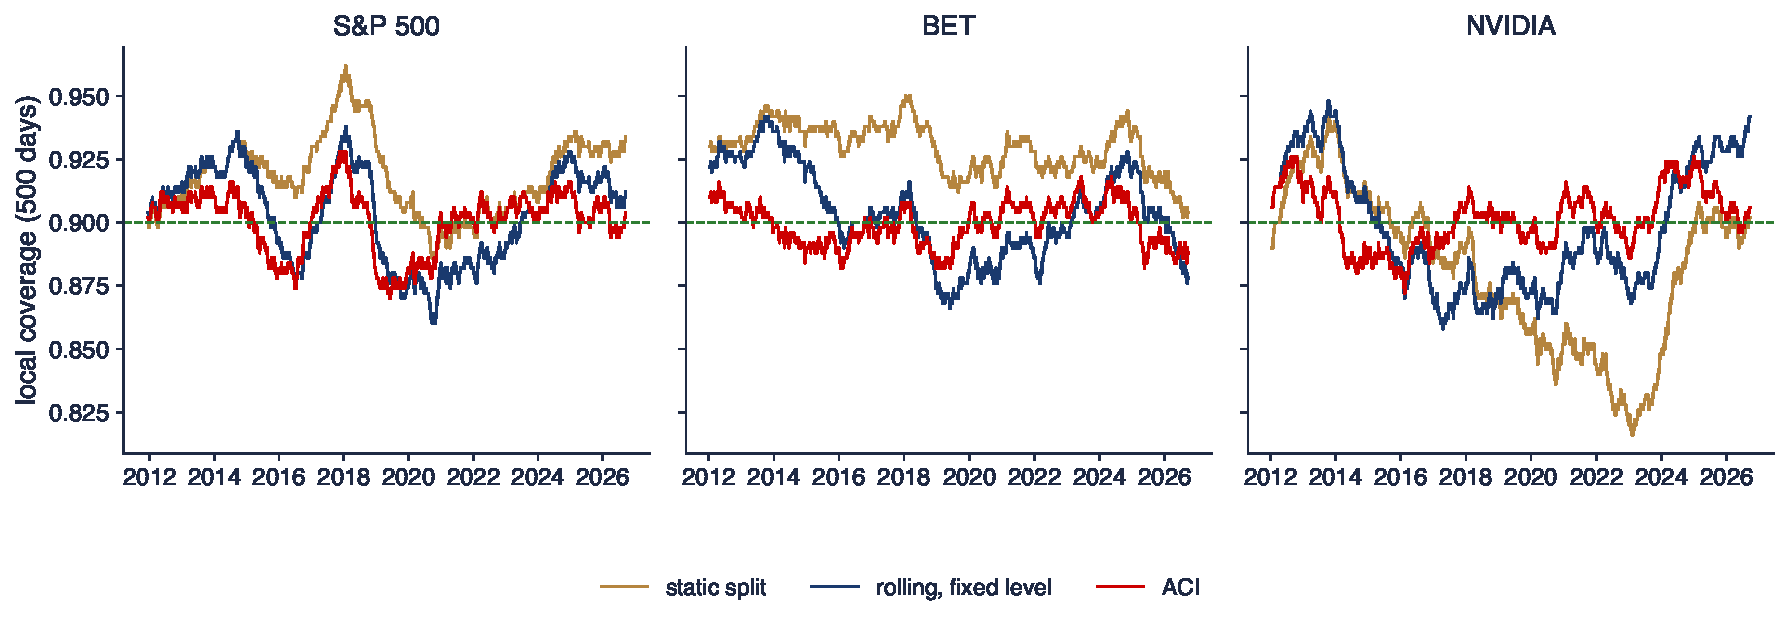
\includegraphics[width=0.97\textwidth,height=0.46\textheight,keepaspectratio]{ats_ch13_aci.pdf}
\end{center}
\vspace{-0.25cm}
\begin{itemize}
    \item Designul din \refGC: $V_t = r_t^2$, $\hat\sigma_t^2$ dintr-un GARCH(1,1) estimat pe ultimele 1250 de zile, scorul $|V_t - \hat\sigma_t^2|/\hat\sigma_t^2$, $\alpha = 0{,}1$, $\gamma = 0{,}005$; acoperirea locală pe 500 de zile; evaluare din 15 decembrie 2009
\end{itemize}
\quantlet{ATS\_ch13\_conformal\_time}{\qlurl{ATS_ch13_conformal_time}}
\end{frame}

\begin{frame}{Interpretarea ACI pe volatilitate}
\itemsize{\small}
\begin{itemize}
    \item Acoperirea totală, S\&P 500: static 0{,}918, mobil 0{,}903, ACI 0{,}901; BET: 0{,}928; 0{,}903; 0{,}899; NVIDIA: 0{,}882; 0{,}900; 0{,}901
    \item Acoperirea locală a metodei statice variază între 0{,}884 și 0{,}962 (S\&P 500); ACI rămîne între 0{,}870 și 0{,}928
    \item Acoperirea condiționată Christoffersen pentru ratări (S\&P 500): static $p$ $<$ 0{,}001, ACI $p$ = 0{,}968: o calibrare fixată pe 2005--2009 este prea largă ulterior; actualizarea reface atît frecvența, cît și independența ratărilor
\end{itemize}
\end{frame}

\begin{frame}{Pasul ACI}
\itemsize{\footnotesize}
\begin{center}
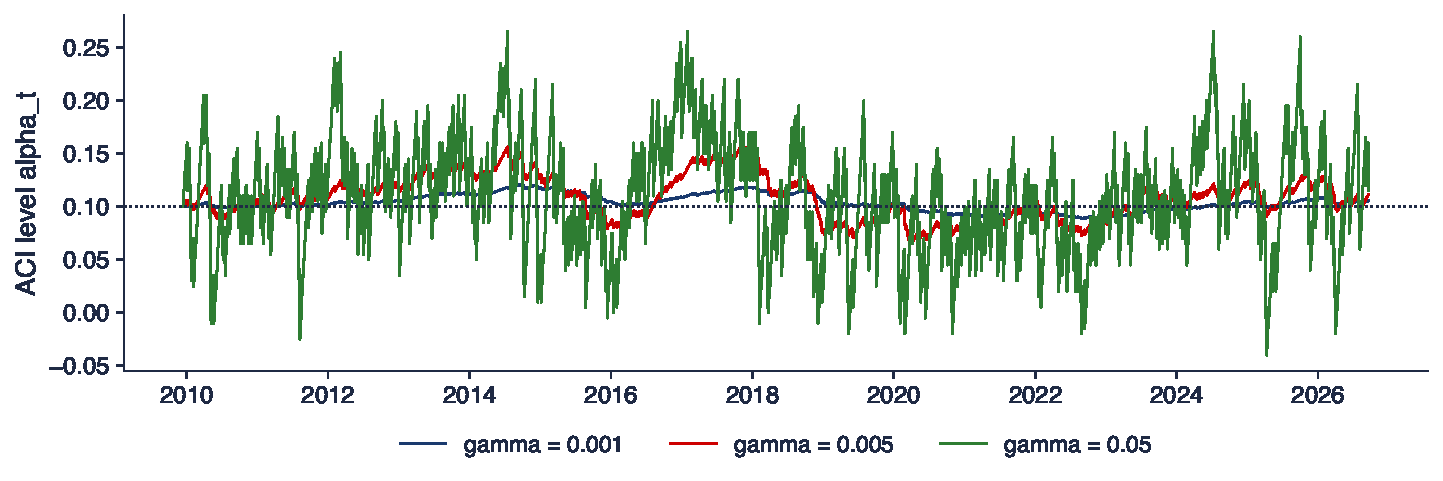
\includegraphics[width=0.97\textwidth,height=0.46\textheight,keepaspectratio]{ats_ch13_aci_gamma.pdf}
\end{center}
\vspace{-0.25cm}
\begin{itemize}
    \item Scorurile S\&P 500 din graficul anterior: nivelul $\alpha_t$ pentru $\gamma = 0{,}001$, 0,005 și 0,05
\end{itemize}
\quantlet{ATS\_ch13\_conformal\_time}{\qlurl{ATS_ch13_conformal_time}}
\end{frame}

\begin{frame}{Interpretarea pasului}
\itemsize{\small}
\begin{itemize}
    \item Frecvențele ratărilor 0{,}0987; 0{,}0994; 0{,}0999 față de marginile 0{,}2138; 0{,}0430; 0{,}0045 ($T = 4214$): teorema este respectată cu o marjă largă
    \item $\gamma$ mare: $\alpha_t$ variază între \ensuremath{-}0{,}04 și 0{,}27, intervale infinite în 1{,}6\% din zile; $\gamma$ mic: reacție lentă, serii lungi de ratări după un șoc
    \item $\gamma$ echilibrează adaptivitatea și stabilitatea: alegeți-l pe o fereastră trecută sau lăsați DtACI să agrege mai multe valori
\end{itemize}
\end{frame}

\begin{frame}{Controlul PID conformal}
\itemsize{\small}
\begin{itemize}
    \item \refACT: \textbf{urmărirea cuantilei} (P): $q_{t+1} = q_t + \eta(\mathrm{err}_t - \alpha)$, adică coborîre pe gradient online pe pierderea pinball a scorului
    \begin{itemize}
        \item \textbf{Propoziție}: dacă $S_t \in [0, B]$, atunci $\big|\frac1T\sum_t(\mathrm{err}_t - \alpha)\big| \le (B + \eta)/(\eta T)$: pragul se mișcă pe scala scorurilor, nu a lui $\alpha$
    \end{itemize}
    \item \textbf{Integratorul} (I): se adaugă $r_t\big(\sum_{i \le t}(\mathrm{err}_i - \alpha)\big)$, $r_t(x) = K_I\tan\big(x\log t/(tC_{\mathrm{sat}})\big)$: reacționează la eroarea de acoperire acumulată și se saturează pentru a păstra garanția
    \item \textbf{Prognozatorul de scor} (asemănător termenului D): un model care prognozează scorul următor din trecutul lui (sezonalitate, tendințe ale erorilor) și se adaugă la prag
    \item ACI este cazul particular care urmărește nivelul în loc de cuantilă; PID își ia vocabularul din ingineria controlului: proporțional, integral, derivat
\end{itemize}
\end{frame}

\begin{frame}{Metode online pe consumul României}
\itemsize{\footnotesize}
\begin{center}
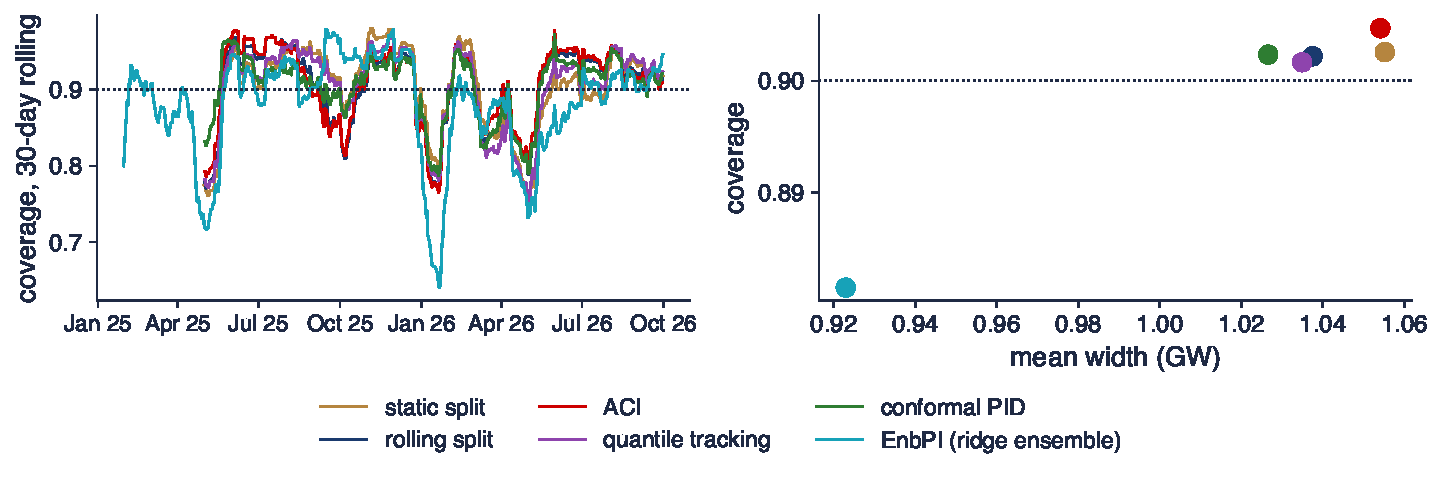
\includegraphics[width=0.97\textwidth,height=0.48\textheight,keepaspectratio]{ats_ch13_pid.pdf}
\end{center}
\vspace{-0.25cm}
\begin{itemize}
    \item Intervale de 90\% pentru ziua următoare în jurul medianei Chronos-Bolt, cîte un flux de scoruri pe oră (24 de fluxuri), fereastra de calibrare 91 de zile; EnbPI pe regresorii ARX expert (ridge, 20 de modele bootstrap pe blocuri); evaluare din 2 aprilie 2025
\end{itemize}
\quantlet{ATS\_ch13\_conformal\_time}{\qlurl{ATS_ch13_conformal_time}}
\end{frame}

\begin{frame}{Interpretarea metodelor online}
\itemsize{\small}
\begin{itemize}
    \item Acoperirea: static 0{,}903, mobil 0{,}902, ACI 0{,}905, urmărirea cuantilei 0{,}902, PID 0{,}902, EnbPI 0{,}881
    \item Lățimea medie (GW): 1{,}06; 1{,}04; 1{,}05; 1{,}03; 1{,}03; 0{,}92; cea mai slabă acoperire pe 30 de zile: static 0{,}747, PID 0{,}787
    \item Pe toată perioada, toate metodele în afară de EnbPI sînt aproape de 90\%; diferențele țin de scăderile după tranzițiile sezoniere și de lățime, iar PID este cel mai bun la ambele
    \item EnbPI centrează banda pe propriul ansamblu ridge, mai puțin precis decît prognoza de bază: intervale mai înguste, acoperire mai mică
\end{itemize}
\end{frame}

\begin{frame}{Diagnosticarea acoperirii}
\itemsize{\small}
\begin{itemize}
    \item \textbf{Necondiționat}: frecvența ratărilor și testul Kupiec \refKup; \textbf{independența} ratărilor: Christoffersen \refChr{} (\atschlink{https://danpele.github.io/Advanced-Time-Series/RO/Cursuri/capitol9_var_es_backtesting.pdf}{Capitolul 9})
    \begin{itemize}
        \item o verificare prin regresie în spiritul testului DQ \refEM: regresia lui $\mathrm{err}_t - \alpha$ pe ratările decalate și pe lățimea prognozată
    \end{itemize}
    \item \textbf{Local}: acoperirea pe ferestre mobile; acoperirea pe clase ale unei variabile cunoscute la origine (volatilitatea prognozată, ora, regimul): echivalentul empiric al acoperirii condiționate
    \item \textbf{Precizia}: lățimea medie și scorul de interval $W + \frac{2}{\alpha}(\ell - y)\mathbf 1\{y < \ell\} + \frac{2}{\alpha}(y - u)\mathbf 1\{y > u\}$ \refWin, \refGR, un scor propriu pentru intervale centrale
    \item Raportați toate trei: o metodă validă, dar de două ori mai largă, nu este o metodă mai bună
\end{itemize}
\end{frame}

\begin{frame}{Acoperirea pe regimuri de volatilitate}
\itemsize{\footnotesize}
\begin{center}
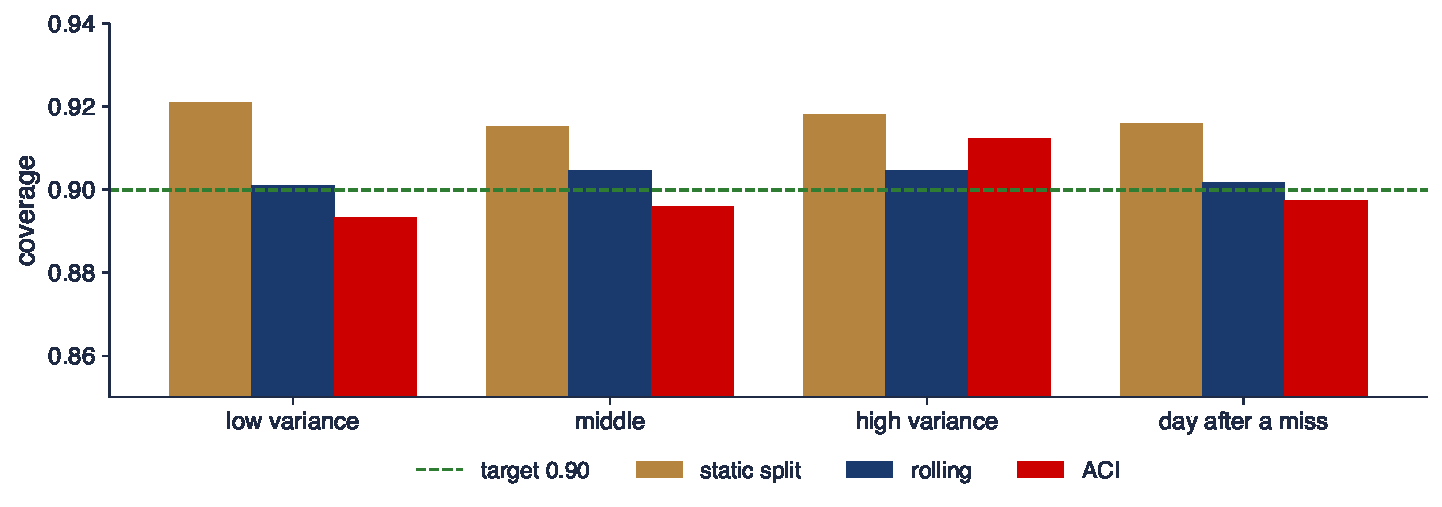
\includegraphics[width=0.97\textwidth,height=0.46\textheight,keepaspectratio]{ats_ch13_condcov.pdf}
\end{center}
\vspace{-0.25cm}
\begin{itemize}
    \item S\&P 500, intervalele de volatilitate de 90\% din graficul ACI: acoperirea pe terțile ale varianței prognozate de GARCH și în ziua de după o ratare
\end{itemize}
\quantlet{ATS\_ch13\_conformal\_time}{\qlurl{ATS_ch13_conformal_time}}
\end{frame}

\begin{frame}{Interpretarea acoperirii condiționate}
\itemsize{\small}
\begin{itemize}
    \item Static: 0{,}921 (varianță mică), 0{,}918 (mare), 0{,}916 după o ratare; ACI: 0{,}893; 0{,}912; 0{,}897
    \item Acoperirea este aproape constantă pe terțile de volatilitate și după o ratare, pentru toate metodele: împărțirea la varianța GARCH face scorul aproape pivotal
    \item Contrast: cu scorul brut $|r_t|$ (Seminarul 13, B3) ratările se grupează în anii agitați, oricare ar fi calibrarea; acoperirea condiționată este o proprietate a scorului, nu a pasului conformal
\end{itemize}
\end{frame}

\begin{frame}{Recapitulare: metodele conformale pentru serii de timp}
\itemsize{\small}
\begin{itemize}
    \item Conformal ponderat: o margine a acoperirii exprimată prin variația totală; ponderile geometrice se adaptează derivei
    \item EnbPI: ansambluri bootstrap și o fereastră mobilă de reziduuri, validitate asimptotică sub mixing
    \item ACI și PID: reacția la ratări dă acoperire pe termen lung pentru orice șir; acoperirea condiționată trebuie totuși testată
\end{itemize}
\end{frame}


%=============================================================================
\section{Calibrarea intervalelor produse de foundation models}
%=============================================================================

\begin{frame}{Nevoia de calibrare a cuantilelor foundation models}
\itemsize{\small}
\begin{itemize}
    \item Cuantilele preantrenate sînt calibrate pe distribuția corpusului, nu pe seria dumneavoastră: calibrarea greșită este situația implicită, în ambele sensuri
    \item Majoritatea modelelor dau doar cuantile de 10\%--90\%: un interval de 95\% sau VaR 1\% cere extrapolare dincolo de nivelurile antrenate
    \item Rețeta: CQR online pe banda proprie a modelului, scorul $S_t = \max\{\hat q_{0{,}1,t} - y_t, y_t - \hat q_{0{,}9,t}\}$; ACI alege pragul pentru orice nivel-țintă ($80\%$ sau $95\%$)
    \begin{itemize}
        \item varianta unilaterală pentru VaR: $S_t = \hat q_{0{,}1,t} - y_t$, pragul la nivelul $\alpha$; VaR este $-(\hat q_{0{,}1,t} - q_t)$
    \end{itemize}
    \item Lectură suplimentară despre recalibrarea conformală a VaR pentru foundation models: \refCO; \refTV
\end{itemize}
\end{frame}

\begin{frame}{Acoperirea brută și cea conformală a foundation models}
\itemsize{\footnotesize}
\begin{center}
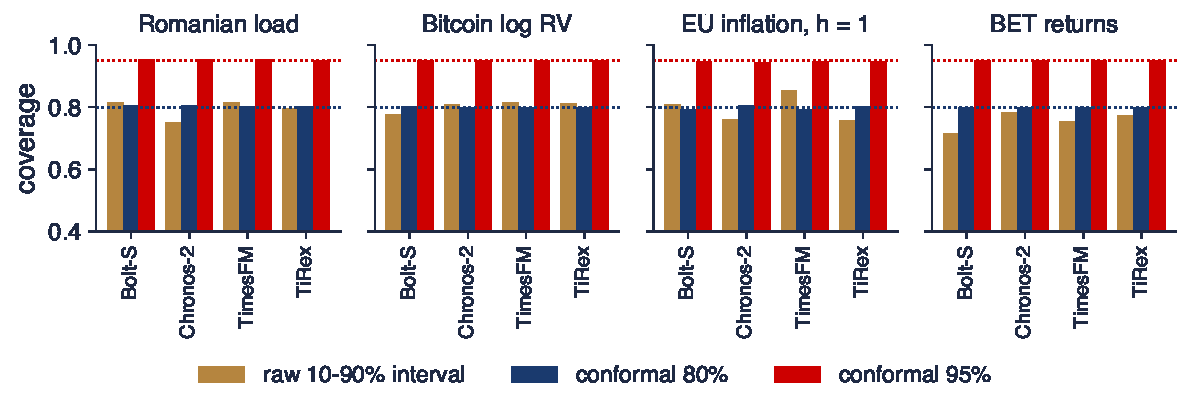
\includegraphics[width=0.97\textwidth,height=0.48\textheight,keepaspectratio]{ats_ch13_fm_calib.pdf}
\end{center}
\vspace{-0.25cm}
\begin{itemize}
    \item Acoperirea benzii brute de 10--90\% și a intervalelor CQR online de 80\% și 95\% (ACI, fereastra 250, $\gamma = 0{,}005$): consumul României (24 de fluxuri orare), log RV Bitcoin, inflația UE la $h = 1$ (27 de fluxuri), randamentele zilnice BET
\end{itemize}
\quantlet{ATS\_ch13\_calibration}{\qlurl{ATS_ch13_calibration}}
\end{frame}

\begin{frame}{Interpretarea calibrării}
\itemsize{\small}
\begin{itemize}
    \item Benzile brute de 80\%: consum 75--81\%, Bitcoin 77--81\%, inflație 76--85\%, randamente BET 72--78\% pentru cele patru modele
    \item După CQR online: intervalele de 80\% acoperă 79--81\%, cele de 95\% 94{,}5--95{,}4\% în toate sarcinile
    \item Benzile brute greșesc în ambele sensuri (prea înguste: Chronos-2 la consum; prea largi: TimesFM la inflație); pasul conformal le lărgește sau le îngustează, cu o lățime medie între 0{,}90 și 1{,}24 ori lățimea brută, și ajunge la 95\% pornind de la modele care produc doar decile
\end{itemize}
\end{frame}

\begin{frame}{Valoarea la risc din foundation models}
\itemsize{\footnotesize}
\begin{center}
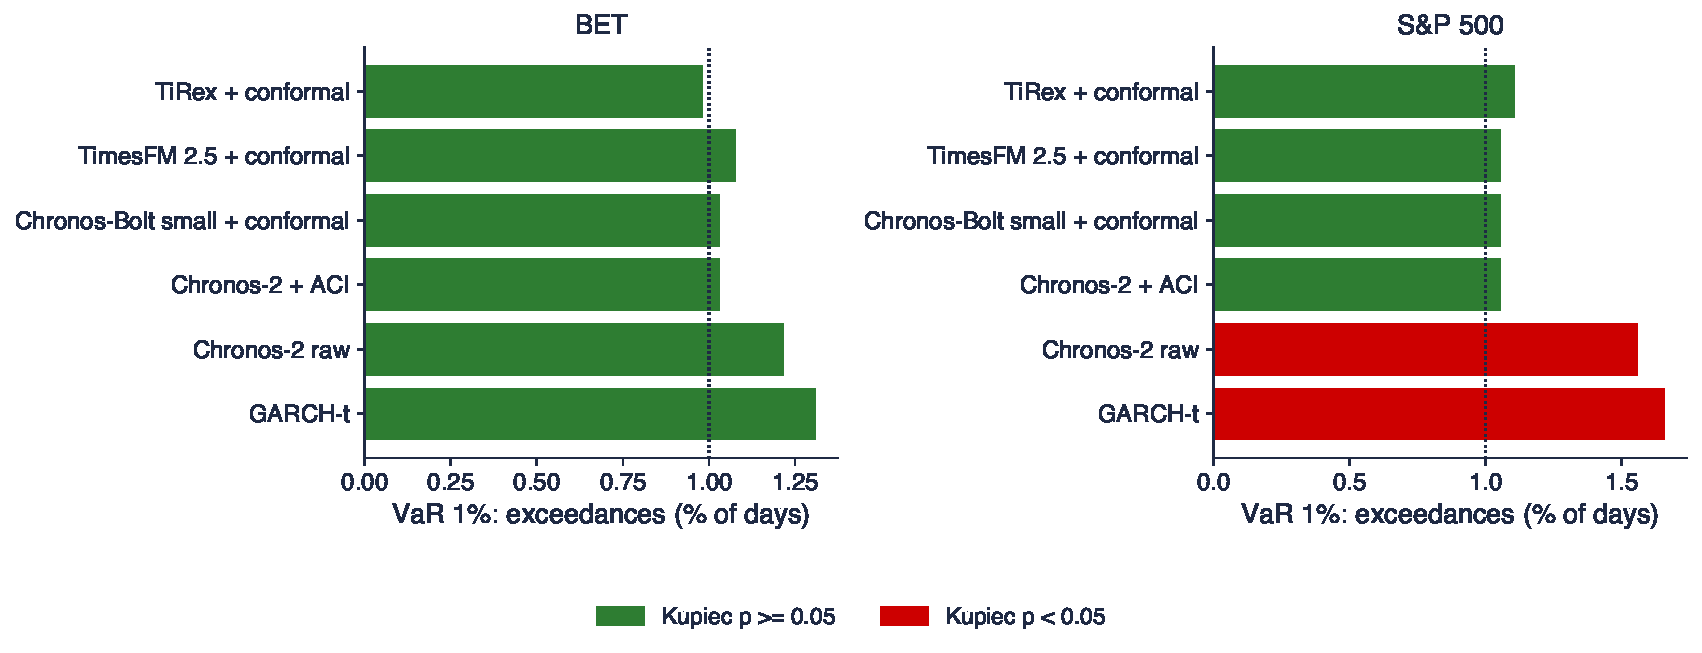
\includegraphics[width=0.97\textwidth,height=0.48\textheight,keepaspectratio]{ats_ch13_fm_var.pdf}
\end{center}
\vspace{-0.25cm}
\begin{itemize}
    \item Depășirile VaR 1\%, BET și S\&P 500 din 28 decembrie 2017 (2\,175 de zile): GARCH-$t$ (fereastră mobilă de 1000 de zile, \atschlink{https://danpele.github.io/Advanced-Time-Series/RO/Cursuri/capitol9_var_es_backtesting.pdf}{Capitolul 9}), Chronos-2 brut și cu ACI, decilele celorlalte modele extinse printr-o deplasare conformală unilaterală
\end{itemize}
\quantlet{ATS\_ch13\_calibration}{\qlurl{ATS_ch13_calibration}}
\end{frame}

\begin{frame}{Interpretarea backtesting-ului VaR}
\itemsize{\small}
\begin{itemize}
    \item BET, VaR 1\%: GARCH-$t$ 1{,}31\% (Kupiec $p$ = 0{,}170), Chronos-2 brut 1{,}22\% ($p$ = 0{,}331), Chronos-2 + ACI 1{,}03\% ($p$ = 0{,}893), TimesFM + conformal 1{,}08\%
    \item S\&P 500: GARCH-$t$ 1{,}66\% (Kupiec $p$ = 0{,}007), Chronos-2 brut 1{,}56\% ($p$ = 0{,}021), + ACI 1{,}06\% ($p$ = 0{,}802, $p$ Christoffersen = 0{,}454)
    \item Calibrarea corectează rata de depășire a oricărui model; nu adaugă informație despre coadă: decilele extinse conformal au o pierdere cuantilică mai mare decît GARCH-$t$ (BET, Chronos-Bolt: DM $t = 2{,}70$), în timp ce Chronos-2, antrenat pe cuantile de 1\%, nu are ($t = 0{,}10$)
\end{itemize}
\end{frame}

\begin{frame}{Recapitulare: calibrarea}
\itemsize{\small}
\begin{itemize}
    \item Tratați cuantilele foundation models ca scoruri de calibrat, nu ca probabilități
    \item CQR online cu ACI dă acoperirea-țintă la orice nivel, inclusiv dincolo de cuantilele antrenate
    \item Testați VaR calibrat ca în \atschlink{https://danpele.github.io/Advanced-Time-Series/RO/Cursuri/capitol9_var_es_backtesting.pdf}{Capitolul 9}: frecvență, independență și pierdere
\end{itemize}
\end{frame}


%=============================================================================
\section{AI în descoperirea științifică}
%=============================================================================

\begin{frame}{O întrebare deschisă}
\itemsize{\small}
\begin{itemize}
    \item Întrec foundation models pentru serii de timp modelele econometrice de domeniu pe datele din Europa Centrală și de Est, într-o fereastră de după lansarea lor și cu corecție pentru testarea multiplă?
    \begin{itemize}
        \item formal: $H_0$: pierderea așteptată egală (agregată pe serii preînregistrate) a celui mai bun foundation model și a celui mai bun model de domeniu, într-o fereastră care începe după lansarea tuturor modelelor
        \item infirmată de un test DM agregat la 5\% și de un MCS care exclude una dintre părți, pe serii și orizonturi fixate înainte de sosirea datelor
    \end{itemize}
    \item De ce contează: băncile centrale și operatorii de rețea iau în calcul înlocuirea modelelor ajustate cu modele zero-shot; cîștigurile publicate provin adesea dintr-o alegere favorabilă a seriilor
    \begin{itemize}
        \item literatura de pornire: \refAks, \refShc, \refMey, \refPE, \refBri
    \end{itemize}
\end{itemize}
\end{frame}

\begin{frame}{Bucla de cercetare cu un asistent AI}
\itemsize{\footnotesize}
\begin{itemize}
    \item Un asistent AI (un LLM precum Claude, ChatGPT, Gemini sau Copilot) accelerează fiecare etapă; Semantic Scholar și Elicit ajută la literatură
    \begin{itemize}
        \item \textbf{literatura}: \aiprompt{Listează articole recenzate sau de pe arXiv din 2024 încoace care evaluează foundation models pentru serii de timp doar după datele lor de lansare; dă identificatorii arXiv sau DOI.} Apoi verificați fiecare identificator
        \item \textbf{ipoteza}: \aiprompt{Scrie o preînregistrare: seriile, originile, orizonturile, funcțiile de pierdere, modelele de referință, testul agregat și nivelul MCS.}
        \item \textbf{cod și replicare}: cereți o funcție care întoarce cuantile la niveluri fixe pentru fiecare model; reproduceți întîi o cifră cunoscută (domeniul cuantilelor Chronos-Bolt, MAE-ul nostru pentru consum)
        \item \textbf{critica}: \aiprompt{Joacă rolul unui recenzent ostil: enumeră toate felurile în care acest benchmark ar putea favoriza foundation models.}
    \end{itemize}
    \item Raportul: ce s-a cerut, ce s-a păstrat, ce s-a respins (AI\_USE.md, AI\_ERRORS.md)
\end{itemize}
\end{frame}

\begin{frame}{Verificări necesare}
\itemsize{\small}
\begin{itemize}
    \item Fiecare referință există și spune ce se afirmă (identificatorul arXiv sau DOI funcționează, titlul coincide, rezultatul se află în lucrare)
    \item Datele de lansare și datele-limită de antrenare ale fiecărui model, din fișele modelelor, comparate cu începutul ferestrei de evaluare
    \item Nivelurile de cuantile produse efectiv de fiecare model (o cerere pentru 1\% poate întoarce, fără avertisment, 10\%)
    \item Modelele de referință ajustate cu aceeași grijă; contextul disponibil este același pentru toate modelele
    \item Multiplicitatea: numărul de serii, orizonturi și modele testate; raportarea testului agregat și a valorilor $p$ ajustate
\end{itemize}
\end{frame}

\begin{frame}{Mini studiu de caz: cît poate schimba verdictul alegerea benchmark-ului?}
\itemsize{\footnotesize}
\begin{center}
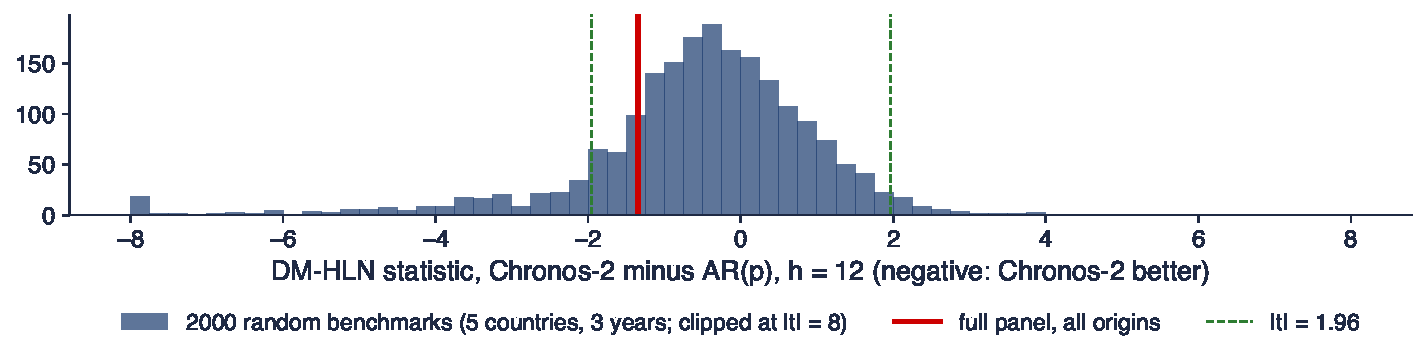
\includegraphics[width=0.97\textwidth,height=0.4\textheight,keepaspectratio]{ats_ch13_ai_case.pdf}
\end{center}
\vspace{-0.25cm}
\begin{itemize}
    \item Statisticile DM--HLN ale Chronos-2 față de AR($p$) la $h = 12$ pe 2000 de benchmark-uri aleatoare cu 5 țări UE și 3 ani de origini și pe întregul panel
    \item 11{,}2\% dintre benchmark-urile aleatoare declară Chronos-2 semnificativ mai bun, iar 2{,}1\% semnificativ mai slab; panelul întreg dă $t = \ensuremath{-}1{,}35$ ($p$ = 0{,}180). Un rezumat AI care prezintă o astfel de lucrare ca dovadă pentru (sau împotriva) foundation models greșește; doar panelul preînregistrat răspunde
\end{itemize}
\quantlet{ATS\_ch13\_benchmark}{\qlurl{ATS_ch13_benchmark}}
\end{frame}

\begin{frame}{Idee de proiect}
\itemsize{\small}
\begin{itemize}
    \item \textbf{Un benchmark preînregistrat, de după lansare, al foundation models pentru macroeconomia și riscul din Europa Centrală și de Est, cu calibrare conformală}
    \begin{itemize}
        \item replicați: protocolul zero-shot din \refAns{} (WQL, MASE, medii geometrice) și designul ACI pentru volatilitate din \refGC{} pe datele noastre
        \item extindeți: inflația, consumul și indicii bursieri din România, Polonia, Ungaria și Cehia; covariabile în context (prețurile energiei, calendare); CQR online pentru 95\% și VaR 1\%; teste agregate cu Holm și BH
        \item preînregistrați: seriile, originile după 1 noiembrie 2025, orizonturile, funcțiile de pierdere, modelele de referință și regula de decizie; prognozele pentru lunile următoare se notează înainte de sosirea datelor
    \end{itemize}
    \item Livrabilele urmează regulile cursului: repository, raport, AI\_USE.md, AI\_ERRORS.md, susținere orală
\end{itemize}
\end{frame}


%=============================================================================
\section{Încheiere}
%=============================================================================

\begin{frame}{Idei de reținut}
\itemsize{\small}
\begin{itemize}
    \item Foundation models amortizează estimarea pe un corpus; alegerile de proiectare (scalarea, patch-urile, domeniul cuantilelor) stabilesc ce pot și ce nu pot prognoza
    \item Pe datele noastre cel mai bun model zero-shot este competitiv cu modelele de domeniu; cîștigurile depind de sarcină și nu rezistă alegerii selective
    \item Evaluați după lansare, agregați pe serii, corectați pentru multiplicitate
    \item Predicția conformală dă acoperire marginală în eșantioane finite sub interschimbabilitate; sub dependență, ponderile, ansamblurile și reacția la erori refac acoperirea pe termen lung
    \item Acoperirea condiționată este imposibilă în general: diagnosticați-o cu testele Christoffersen și cu acoperirea pe regimuri
\end{itemize}
\end{frame}

\begin{frame}{Autoevaluare}
\itemsize{\small}
\begin{columns}[T]
\begin{column}{0.56\textwidth}
\begin{block}{Întrebări}
\begin{itemize}
    \item De ce nu poate Chronos să prognozeze o valoare peste $15s$?
    \item De ce încalcă un AR(1) staționar interschimbabilitatea?
    \item Care este legea acoperirii split conformal condiționată de setul de calibrare?
    \item Ce mărime rămîne mărginită în demonstrația teoremei ACI?
    \item De ce este necesară o fereastră de după lansare într-un benchmark al foundation models?
\end{itemize}
\end{block}
\end{column}
\begin{column}{0.40\textwidth}
\begin{block}{Urmează: \atschlink{https://danpele.github.io/Advanced-Time-Series/RO/Cursuri/capitol14_inferenta_cauzala_serii_timp.pdf}{Capitolul 14}}
\begin{itemize}
    \item Inferență cauzală pentru serii de timp
    \item cauzalitatea Granger și cea structurală, descoperirea relațiilor cauzale, evaluarea politicilor
\end{itemize}
\end{block}
\end{column}
\end{columns}
\end{frame}


%=============================================================================
\section{Anexă}
%=============================================================================

\begin{frame}{Anexă: demonstrația acoperirii split conformal}
\hypertarget{atsapp1}{}\atsappback{atssrc1}{Înapoi}
\itemsize{\small}
\begin{itemize}
    \item Condiționăm pe setul de antrenare, astfel încît $\hat\mu$ și $s$ sînt fixate; interschimbabilitatea lui $Z_1, \dots, Z_{n+1}$ implică interschimbabilitatea lui $S_1, \dots, S_{n+1}$
    \item Fără egalități, rangul $R$ al lui $S_{n+1}$ printre $S_1, \dots, S_{n+1}$ este uniform pe $\{1, \dots, n + 1\}$ (orice ordonare este la fel de probabilă)
    \item $S_{n+1} \le S_{(k)}$ (statistica de ordine a primelor $n$) $\iff R \le k$; deci $\Pr\{Y_{n+1} \in \hat C\} = k/(n + 1)$
    \item $k = \lceil (n + 1)(1 - \alpha)\rceil$ dă $1 - \alpha \le k/(n + 1) < 1 - \alpha + 1/(n + 1)$; egalitățile doar cresc acoperirea
    \item Condiționat de setul de calibrare, acoperirea este $F(S_{(k)})$, unde $F$ este distribuția scorului; $F(S_i)$ sînt uniforme i.i.d., deci $F(S_{(k)}) \sim$ Beta($k$, $n + 1 - k$)
\end{itemize}
\end{frame}

\begin{frame}{Anexă: cele două garanții online}
\hypertarget{atsapp2}{}\atsappback{atssrc1}{Înapoi}
\itemsize{\small}
\begin{itemize}
    \item \textbf{ACI}: dacă $\alpha_t < 0$, atunci $q_t = +\infty$ și $\mathrm{err}_t = 0$, deci $\alpha_{t+1} = \alpha_t + \gamma\alpha > \alpha_t$; dacă $\alpha_t > 1$, $\mathrm{err}_t = 1$ și $\alpha_t$ scade
    \begin{itemize}
        \item deci $\alpha_t \in [-\gamma, 1 + \gamma]$ pentru orice $t$; însumînd actualizările, $\gamma\big|\sum_{t \le T}(\alpha - \mathrm{err}_t)\big| = |\alpha_{T+1} - \alpha_1| \le \max\{\alpha_1, 1 - \alpha_1\} + \gamma$
    \end{itemize}
    \item \textbf{Urmărirea cuantilei}: dacă $q_t > B$, atunci $\mathrm{err}_t = 0$ și $q_t$ scade cu $\eta\alpha$; dacă $q_t < 0$, atunci $\mathrm{err}_t = 1$ și $q_t$ crește
    \begin{itemize}
        \item deci $q_t \in [-\eta, B + \eta]$ (pornind din interior); $\eta\sum_{t \le T}(\mathrm{err}_t - \alpha) = q_{T+1} - q_1$, deci abaterea medie este cel mult $(B + \eta)/(\eta T)$
    \end{itemize}
    \item Niciuna dintre demonstrații nu folosește probabilități: garanțiile sînt valabile pentru orice șir, motiv pentru care nu spun nimic despre acoperirea condiționată
\end{itemize}
\end{frame}


%=============================================================================
\section{Bibliografie}
%=============================================================================

\begin{frame}{Bibliografie (1/6)}
\itemsize{\tiny}
\begin{itemize}
    \item Aksu, T., Woo, G., Liu, J., Liu, X., Liu, C., Savarese, S., Xiong, C., \& Sahoo, D. (2024). GIFT-Eval: A benchmark for general time series forecasting model evaluation. \textit{arXiv:2410.10393}. \href{https://arxiv.org/abs/2410.10393}{arXiv:2410.10393}
    \item Angelopoulos, A. N., \& Bates, S. (2023). Conformal prediction: A gentle introduction. \textit{Foundations and Trends in Machine Learning}, 16(4), 494--591. \href{https://doi.org/10.1561/2200000101}{doi:10.1561/2200000101}
    \item Angelopoulos, A. N., Candès, E. J., \& Tibshirani, R. J. (2023). Conformal PID control for time series prediction. \textit{Advances in Neural Information Processing Systems 36}; \textit{arXiv:2307.16895}. \href{https://arxiv.org/abs/2307.16895}{arXiv:2307.16895}
    \item Ansari, A. F., Shchur, O., Küken, J., Auer, A., Han, B., Mercado, P., et al.\ (2025). Chronos-2: From univariate to universal forecasting. \textit{arXiv:2510.15821}. \href{https://arxiv.org/abs/2510.15821}{arXiv:2510.15821}
    \item Ansari, A. F., Stella, L., Turkmen, C., Zhang, X., Mercado, P., Shen, H., et al.\ (2024). Chronos: Learning the language of time series. \textit{Transactions on Machine Learning Research}; \textit{arXiv:2403.07815}. \href{https://arxiv.org/abs/2403.07815}{arXiv:2403.07815}
    \item Auer, A., Podest, P., Klotz, D., Böck, S., Klambauer, G., \& Hochreiter, S. (2025). TiRex: Zero-shot forecasting across long and short horizons with enhanced in-context learning. \textit{Advances in Neural Information Processing Systems}; \textit{arXiv:2505.23719}. \href{https://arxiv.org/abs/2505.23719}{arXiv:2505.23719}
    \item Barber, R. F., Candès, E. J., Ramdas, A., \& Tibshirani, R. J. (2023). Conformal prediction beyond exchangeability. \textit{The Annals of Statistics}, 51(2), 816--845. \href{https://doi.org/10.1214/23-AOS2276}{doi:10.1214/23-AOS2276}
    \item Benjamini, Y., \& Hochberg, Y. (1995). Controlling the false discovery rate: A practical and powerful approach to multiple testing. \textit{Journal of the Royal Statistical Society: Series B}, 57(1), 289--300. \href{https://doi.org/10.1111/j.2517-6161.1995.tb02031.x}{doi:10.1111/j.2517-6161.1995.tb02031.x}
    \item Bollerslev, T. (1986). Generalized autoregressive conditional heteroskedasticity. \textit{Journal of Econometrics}, 31(3), 307--327. \href{https://doi.org/10.1016/0304-4076(86)90063-1}{doi:10.1016/0304-4076(86)90063-1}
    \item Bommasani, R., Hudson, D. A., Adeli, E., Altman, R., Arora, S., et al.\ (2021). On the opportunities and risks of foundation models. \textit{arXiv:2108.07258}. \href{https://arxiv.org/abs/2108.07258}{arXiv:2108.07258}
    \item Brini, A. (2026). Forecasting realized volatility with time series foundation models: A comparison with econometric benchmarks. \textit{arXiv:2607.05291}. \href{https://arxiv.org/abs/2607.05291}{arXiv:2607.05291}
    \item Chernozhukov, V., Wüthrich, K., \& Zhu, Y. (2018). Exact and robust conformal inference methods for predictive machine learning with dependent data. \textit{Proceedings of the 31st Conference on Learning Theory (COLT)}; \textit{arXiv:1802.06300}. \href{https://arxiv.org/abs/1802.06300}{arXiv:1802.06300}
    \item Christoffersen, P. F. (1998). Evaluating interval forecasts. \textit{International Economic Review}, 39(4), 841--862. \href{https://doi.org/10.2307/2527341}{doi:10.2307/2527341}
    \item Cohen, B., Khwaja, E., Doubli, Y., Lemaachi, S., Lettieri, C., Masson, C., et al.\ (2025). This time is different: An observability perspective on time series foundation models. \textit{arXiv:2505.14766}. \href{https://arxiv.org/abs/2505.14766}{arXiv:2505.14766}
\end{itemize}
\end{frame}

\begin{frame}{Bibliografie (2/6)}
\itemsize{\tiny}
\begin{itemize}
    \item Corsi, F. (2009). A simple approximate long-memory model of realized volatility. \textit{Journal of Financial Econometrics}, 7(2), 174--196. \href{https://doi.org/10.1093/jjfinec/nbp001}{doi:10.1093/jjfinec/nbp001}
    \item Das, A., Kong, W., Sen, R., \& Zhou, Y. (2024). A decoder-only foundation model for time-series forecasting. \textit{Proceedings of the 41st International Conference on Machine Learning (ICML)}; \textit{arXiv:2310.10688}. \href{https://arxiv.org/abs/2310.10688}{arXiv:2310.10688}
    \item Demšar, J. (2006). Statistical comparisons of classifiers over multiple data sets. \textit{Journal of Machine Learning Research}, 7, 1--30. \href{https://jmlr.org/papers/v7/demsar06a.html}{jmlr.org}
    \item Diebold, F. X., \& Mariano, R. S. (1995). Comparing predictive accuracy. \textit{Journal of Business \& Economic Statistics}, 13(3), 253--263. \href{https://doi.org/10.1080/07350015.1995.10524599}{doi:10.1080/07350015.1995.10524599}
    \item Edwards, T. D. P., Alvey, J., Alsing, J., Nguyen, N. H., \& Wandelt, B. D. (2024). Scaling-laws for large time-series models. \textit{arXiv:2405.13867}. \href{https://arxiv.org/abs/2405.13867}{arXiv:2405.13867}
    \item Engle, R. F., \& Manganelli, S. (2004). CAViaR: Conditional autoregressive value at risk by regression quantiles. \textit{Journal of Business \& Economic Statistics}, 22(4), 367--381. \href{https://doi.org/10.1198/073500104000000370}{doi:10.1198/073500104000000370}
    \item Fleming, P. J., \& Wallace, J. J. (1986). How not to lie with statistics: The correct way to summarize benchmark results. \textit{Communications of the ACM}, 29(3), 218--221. \href{https://doi.org/10.1145/5666.5673}{doi:10.1145/5666.5673}
    \item Foygel Barber, R., Candès, E. J., Ramdas, A., \& Tibshirani, R. J. (2021). The limits of distribution-free conditional predictive inference. \textit{Information and Inference: A Journal of the IMA}, 10(2), 455--482. \href{https://doi.org/10.1093/imaiai/iaaa017}{doi:10.1093/imaiai/iaaa017}
    \item Garza, A., Challu, C., \& Mergenthaler-Canseco, M. (2023). TimeGPT-1. \textit{arXiv:2310.03589}. \href{https://arxiv.org/abs/2310.03589}{arXiv:2310.03589}
    \item Garza, A., Rosillo, R., Mendoza-Smith, R., Salinas, D., Williams, A. R., Ashok, A., Goswami, M., et al.\ (2026). Impermanent: A live benchmark for temporal generalization in time series forecasting. \textit{arXiv:2603.08707}. \href{https://arxiv.org/abs/2603.08707}{arXiv:2603.08707}
    \item Giacomini, R., \& White, H. (2006). Tests of conditional predictive ability. \textit{Econometrica}, 74(6), 1545--1578. \href{https://doi.org/10.1111/j.1468-0262.2006.00718.x}{doi:10.1111/j.1468-0262.2006.00718.x}
    \item Gibbs, I., \& Candès, E. (2021). Adaptive conformal inference under distribution shift. \textit{Advances in Neural Information Processing Systems 34}; \textit{arXiv:2106.00170}. \href{https://arxiv.org/abs/2106.00170}{arXiv:2106.00170}
    \item Gibbs, I., \& Candès, E. J. (2024). Conformal inference for online prediction with arbitrary distribution shifts. \textit{Journal of Machine Learning Research}, 25(162), 1--36. \href{https://jmlr.org/papers/v25/22-1218.html}{jmlr.org}
    \item Gneiting, T., \& Raftery, A. E. (2007). Strictly proper scoring rules, prediction, and estimation. \textit{Journal of the American Statistical Association}, 102(477), 359--378. \href{https://doi.org/10.1198/016214506000001437}{doi:10.1198/016214506000001437}
\end{itemize}
\end{frame}

\begin{frame}{Bibliografie (3/6)}
\itemsize{\tiny}
\begin{itemize}
    \item Goel, A., Pasricha, P., Magris, M., \& Kanniainen, J. (2025). Foundation time-series AI model for realized volatility forecasting. \textit{arXiv:2505.11163}. \href{https://arxiv.org/abs/2505.11163}{arXiv:2505.11163}
    \item Goswami, M., Szafer, K., Choudhry, A., Cai, Y., Li, S., \& Dubrawski, A. (2024). MOMENT: A family of open time-series foundation models. \textit{Proceedings of the 41st International Conference on Machine Learning (ICML)}; \textit{arXiv:2402.03885}. \href{https://arxiv.org/abs/2402.03885}{arXiv:2402.03885}
    \item Gruver, N., Finzi, M., Qiu, S., \& Wilson, A. G. (2023). Large language models are zero-shot time series forecasters. \textit{Advances in Neural Information Processing Systems 36}; \textit{arXiv:2310.07820}. \href{https://arxiv.org/abs/2310.07820}{arXiv:2310.07820}
    \item Hansen, P. R., Lunde, A., \& Nason, J. M. (2011). The model confidence set. \textit{Econometrica}, 79(2), 453--497. \href{https://doi.org/10.3982/ECTA5771}{doi:10.3982/ECTA5771}
    \item Harvey, D., Leybourne, S., \& Newbold, P. (1997). Testing the equality of prediction mean squared errors. \textit{International Journal of Forecasting}, 13(2), 281--291. \href{https://doi.org/10.1016/S0169-2070(96)00719-4}{doi:10.1016/S0169-2070(96)00719-4}
    \item Heber, G., Lunde, A., Shephard, N., \& Sheppard, K. (2009). \textit{Oxford-Man Institute's realized library}, version 0.3. Oxford-Man Institute, University of Oxford. \href{https://web.archive.org/web/20220301022212/https://realized.oxford-man.ox.ac.uk/}{web.archive.org}
    \item Hewamalage, H., Ackermann, K., \& Bergmeir, C. (2023). Forecast evaluation for data scientists: Common pitfalls and best practices. \textit{Data Mining and Knowledge Discovery}, 37, 788--832. \href{https://doi.org/10.1007/s10618-022-00894-5}{doi:10.1007/s10618-022-00894-5}
    \item Hoffmann, J., Borgeaud, S., Mensch, A., Buchatskaya, E., et al.\ (2022). Training compute-optimal large language models. \textit{arXiv:2203.15556}. \href{https://arxiv.org/abs/2203.15556}{arXiv:2203.15556}
    \item Holm, S. (1979). A simple sequentially rejective multiple test procedure. \textit{Scandinavian Journal of Statistics}, 6(2), 65--70. \href{https://www.jstor.org/stable/4615733}{jstor.org}
    \item Hong, T., \& Fan, S. (2016). Probabilistic electric load forecasting: A tutorial review. \textit{International Journal of Forecasting}, 32(3), 914--938. \href{https://doi.org/10.1016/j.ijforecast.2015.11.011}{doi:10.1016/j.ijforecast.2015.11.011}
    \item Hyndman, R. J., \& Koehler, A. B. (2006). Another look at measures of forecast accuracy. \textit{International Journal of Forecasting}, 22(4), 679--688. \href{https://doi.org/10.1016/j.ijforecast.2006.03.001}{doi:10.1016/j.ijforecast.2006.03.001}
    \item Hyndman, R. J., Koehler, A. B., Snyder, R. D., \& Grose, S. (2002). A state space framework for automatic forecasting using exponential smoothing methods. \textit{International Journal of Forecasting}, 18(3), 439--454. \href{https://doi.org/10.1016/S0169-2070(01)00110-8}{doi:10.1016/S0169-2070(01)00110-8}
    \item Jin, M., Wang, S., Ma, L., Chu, Z., Zhang, J. Y., Shi, X., et al.\ (2024). Time-LLM: Time series forecasting by reprogramming large language models. \textit{International Conference on Learning Representations (ICLR)}; \textit{arXiv:2310.01728}. \href{https://arxiv.org/abs/2310.01728}{arXiv:2310.01728}
    \item Kaplan, J., McCandlish, S., Henighan, T., Brown, T. B., Chess, B., Child, R., et al.\ (2020). Scaling laws for neural language models. \textit{arXiv:2001.08361}. \href{https://arxiv.org/abs/2001.08361}{arXiv:2001.08361}
\end{itemize}
\end{frame}

\begin{frame}{Bibliografie (4/6)}
\itemsize{\tiny}
\begin{itemize}
    \item Koenker, R., \& Bassett, G. (1978). Regression quantiles. \textit{Econometrica}, 46(1), 33--50. \href{https://doi.org/10.2307/1913643}{doi:10.2307/1913643}
    \item Kupiec, P. H. (1995). Techniques for verifying the accuracy of risk measurement models. \textit{The Journal of Derivatives}, 3(2), 73--84. \href{https://doi.org/10.3905/jod.1995.407942}{doi:10.3905/jod.1995.407942}
    \item Lei, J., G'Sell, M., Rinaldo, A., Tibshirani, R. J., \& Wasserman, L. (2018). Distribution-free predictive inference for regression. \textit{Journal of the American Statistical Association}, 113(523), 1094--1111. \href{https://doi.org/10.1080/01621459.2017.1307116}{doi:10.1080/01621459.2017.1307116}
    \item Lei, J., \& Wasserman, L. (2014). Distribution-free prediction bands for non-parametric regression. \textit{Journal of the Royal Statistical Society: Series B}, 76(1), 71--96. \href{https://doi.org/10.1111/rssb.12021}{doi:10.1111/rssb.12021}
    \item Lim, B., Arık, S. Ö., Loeff, N., \& Pfister, T. (2021). Temporal Fusion Transformers for interpretable multi-horizon time series forecasting. \textit{International Journal of Forecasting}, 37(4), 1748--1764. \href{https://doi.org/10.1016/j.ijforecast.2021.03.012}{doi:10.1016/j.ijforecast.2021.03.012}
    \item Liu, C., Aksu, T., Liu, J., Liu, X., Yan, H., Pham, Q., Savarese, S., et al.\ (2025). Moirai 2.0: When less is more for time series forecasting. \textit{arXiv:2511.11698}. \href{https://arxiv.org/abs/2511.11698}{arXiv:2511.11698}
    \item Lopez-Lira, A., Tang, Y., \& Zhu, M. (2025). The memorization problem: Can we trust LLMs' economic forecasts? \textit{arXiv:2504.14765}. \href{https://arxiv.org/abs/2504.14765}{arXiv:2504.14765}
    \item Makridakis, S., Spiliotis, E., \& Assimakopoulos, V. (2022). M5 accuracy competition: Results, findings, and conclusions. \textit{International Journal of Forecasting}, 38(4), 1346--1364. \href{https://doi.org/10.1016/j.ijforecast.2021.11.013}{doi:10.1016/j.ijforecast.2021.11.013}
    \item Meyer, M., Kaltenpoth, S., Albers, H., Zalipski, K., \& Müller, O. (2025). TS-Arena: A live forecast pre-registration platform. \textit{arXiv:2512.20761}. \href{https://arxiv.org/abs/2512.20761}{arXiv:2512.20761}
    \item Nie, Y., Nguyen, N. H., Sinthong, P., \& Kalagnanam, J. (2023). A time series is worth 64 words: Long-term forecasting with Transformers. \textit{International Conference on Learning Representations (ICLR)}; \textit{arXiv:2211.14730}. \href{https://arxiv.org/abs/2211.14730}{arXiv:2211.14730}
    \item Oliveira, R. I., Orenstein, P., Ramos, T., \& Romano, J. V. (2024). Split conformal prediction and non-exchangeable data. \textit{Journal of Machine Learning Research}, 25; \textit{arXiv:2203.15885}. \href{https://arxiv.org/abs/2203.15885}{arXiv:2203.15885}
    \item Oreshkin, B. N., Carpov, D., Chapados, N., \& Bengio, Y. (2020). N-BEATS: Neural basis expansion analysis for interpretable time series forecasting. \textit{International Conference on Learning Representations (ICLR)}; \textit{arXiv:1905.10437}. \href{https://arxiv.org/abs/1905.10437}{arXiv:1905.10437}
    \item Pan, Z., \& Ezzat, A. A. (2026). Evaluating time series foundation models for electricity price forecasting: Contamination risk, distributional shifts, and covariate dependence. \textit{arXiv:2607.02623}. \href{https://arxiv.org/abs/2607.02623}{arXiv:2607.02623}
    \item Papadopoulos, H., Proedrou, K., Vovk, V., \& Gammerman, A. (2002). Inductive confidence machines for regression. In \textit{Machine Learning: ECML 2002}, Lecture Notes in Computer Science 2430, 345--356. Springer. \href{https://doi.org/10.1007/3-540-36755-1_29}{doi:10.1007/3-540-36755-1\_29}
\end{itemize}
\end{frame}

\begin{frame}{Bibliografie (5/6)}
\itemsize{\tiny}
\begin{itemize}
    \item Patton, A. J. (2011). Volatility forecast comparison using imperfect volatility proxies. \textit{Journal of Econometrics}, 160(1), 246--256. \href{https://doi.org/10.1016/j.jeconom.2010.03.034}{doi:10.1016/j.jeconom.2010.03.034}
    \item Pele, D. T., et al. Conformal\_Oracle: conformal VaR recalibration for time series foundation models and classical models. GitHub repository (further reading). \href{https://github.com/danpele/Conformal_Oracle}{github.com}
    \item Pele, D. T., et al. TSFM\_VaR\_CEE: benchmarking time-series foundation models for VaR and ES forecasting in Central and Eastern European markets. GitHub repository (further reading). \href{https://github.com/danpele/TSFM_VaR_CEE}{github.com}
    \item Petropoulos, F., Apiletti, D., Assimakopoulos, V., Babai, M. Z., et al.\ (2022). Forecasting: Theory and practice. \textit{International Journal of Forecasting}, 38(3), 705--871. \href{https://doi.org/10.1016/j.ijforecast.2021.11.001}{doi:10.1016/j.ijforecast.2021.11.001}
    \item Rahimikia, E., Ni, H., \& Wang, W. (2025). Re(Visiting) time series foundation models in finance. \textit{arXiv:2511.18578}. \href{https://arxiv.org/abs/2511.18578}{arXiv:2511.18578}
    \item Rasul, K., Ashok, A., Williams, A. R., Ghonia, H., Bhagwatkar, R., Khorasani, A., et al.\ (2023). Lag-Llama: Towards foundation models for probabilistic time series forecasting. \textit{arXiv:2310.08278}. \href{https://arxiv.org/abs/2310.08278}{arXiv:2310.08278}
    \item Romano, Y., Patterson, E., \& Candès, E. (2019). Conformalized quantile regression. \textit{Advances in Neural Information Processing Systems 32}; \textit{arXiv:1905.03222}. \href{https://arxiv.org/abs/1905.03222}{arXiv:1905.03222}
    \item Salinas, D., Flunkert, V., Gasthaus, J., \& Januschowski, T. (2020). DeepAR: Probabilistic forecasting with autoregressive recurrent networks. \textit{International Journal of Forecasting}, 36(3), 1181--1191. \href{https://doi.org/10.1016/j.ijforecast.2019.07.001}{doi:10.1016/j.ijforecast.2019.07.001}
    \item Shchur, O., Ansari, A. F., Turkmen, C., Stella, L., Erickson, N., Guerron, P., et al.\ (2025). fev-bench: A realistic benchmark for time series forecasting. \textit{arXiv:2509.26468}. \href{https://arxiv.org/abs/2509.26468}{arXiv:2509.26468}
    \item Shi, J., Ma, Q., Ma, H., \& Li, L. (2024). Scaling law for time series forecasting. \textit{Advances in Neural Information Processing Systems 37}; \textit{arXiv:2405.15124}. \href{https://arxiv.org/abs/2405.15124}{arXiv:2405.15124}
    \item Tan, M., Merrill, M. A., Gupta, V., Althoff, T., \& Hartvigsen, T. (2024). Are language models actually useful for time series forecasting? \textit{Advances in Neural Information Processing Systems 37}; \textit{arXiv:2406.16964}. \href{https://arxiv.org/abs/2406.16964}{arXiv:2406.16964}
    \item Tibshirani, R. J., Barber, R. F., Candès, E. J., \& Ramdas, A. (2019). Conformal prediction under covariate shift. \textit{Advances in Neural Information Processing Systems 32}; \textit{arXiv:1904.06019}. \href{https://arxiv.org/abs/1904.06019}{arXiv:1904.06019}
    \item Vaswani, A., Shazeer, N., Parmar, N., Uszkoreit, J., Jones, L., Gomez, A. N., Kaiser, Ł., \& Polosukhin, I. (2017). Attention is all you need. \textit{Advances in Neural Information Processing Systems 30}; \textit{arXiv:1706.03762}. \href{https://arxiv.org/abs/1706.03762}{arXiv:1706.03762}
    \item Vovk, V. (2012). Conditional validity of inductive conformal predictors. \textit{Proceedings of the Asian Conference on Machine Learning}, PMLR 25, 475--490. \href{https://proceedings.mlr.press/v25/vovk12.html}{proceedings.mlr.press}
\end{itemize}
\end{frame}

\begin{frame}{Bibliografie (6/6)}
\itemsize{\tiny}
\begin{itemize}
    \item Vovk, V., Gammerman, A., \& Shafer, G. (2022). \textit{Algorithmic Learning in a Random World} (2nd ed.). Springer. \href{https://doi.org/10.1007/978-3-031-06649-8}{doi:10.1007/978-3-031-06649-8}
    \item Vovk, V., Gammerman, A., \& Shafer, G. (2005). \textit{Algorithmic Learning in a Random World}. Springer. \href{https://doi.org/10.1007/b106715}{doi:10.1007/b106715}
    \item Winkler, R. L. (1972). A decision-theoretic approach to interval estimation. \textit{Journal of the American Statistical Association}, 67(337), 187--191. \href{https://doi.org/10.1080/01621459.1972.10481224}{doi:10.1080/01621459.1972.10481224}
    \item Woo, G., Liu, C., Kumar, A., Xiong, C., Savarese, S., \& Sahoo, D. (2024). Unified training of universal time series forecasting Transformers. \textit{Proceedings of the 41st International Conference on Machine Learning (ICML)}; \textit{arXiv:2402.02592}. \href{https://arxiv.org/abs/2402.02592}{arXiv:2402.02592}
    \item Xu, C., \& Xie, Y. (2023). Conformal prediction for time series. \textit{IEEE Transactions on Pattern Analysis and Machine Intelligence}, 45(10), 11575--11587. \href{https://doi.org/10.1109/TPAMI.2023.3272339}{doi:10.1109/TPAMI.2023.3272339}
    \item Xu, C., \& Xie, Y. (2021). Conformal prediction interval for dynamic time-series. \textit{Proceedings of the 38th International Conference on Machine Learning (ICML)}, PMLR 139, 11559--11569. \href{https://proceedings.mlr.press/v139/xu21h.html}{proceedings.mlr.press}
    \item Yao, Q., Yang, C.-H. H., Jiang, R., Liang, Y., Jin, M., \& Pan, S. (2025). Towards neural scaling laws for time series foundation models. \textit{International Conference on Learning Representations (ICLR)}; \textit{arXiv:2410.12360}. \href{https://arxiv.org/abs/2410.12360}{arXiv:2410.12360}
    \item Zaffran, M., Dieuleveut, A., Féron, O., Goude, Y., \& Josse, J. (2022). Adaptive conformal predictions for time series. \textit{Proceedings of the 39th International Conference on Machine Learning (ICML)}; \textit{arXiv:2202.07282}. \href{https://arxiv.org/abs/2202.07282}{arXiv:2202.07282}
    \item Zeng, A., Chen, M., Zhang, L., \& Xu, Q. (2023). Are Transformers effective for time series forecasting? \textit{Proceedings of the AAAI Conference on Artificial Intelligence}, 37(9), 11121--11128. \href{https://doi.org/10.1609/aaai.v37i9.26317}{doi:10.1609/aaai.v37i9.26317}
    \item Zhou, T., Niu, P., Wang, X., Sun, L., \& Jin, R. (2023). One fits all: Power general time series analysis by pretrained LM. \textit{Advances in Neural Information Processing Systems 36}; \textit{arXiv:2302.11939}. \href{https://arxiv.org/abs/2302.11939}{arXiv:2302.11939}
    \item Ziel, F., \& Weron, R. (2018). Day-ahead electricity price forecasting with high-dimensional structures: Univariate vs.\ multivariate modeling frameworks. \textit{Energy Economics}, 70, 396--420. \href{https://doi.org/10.1016/j.eneco.2017.12.016}{doi:10.1016/j.eneco.2017.12.016}
\end{itemize}
\end{frame}

\end{document}
